%
% Rapport DAT modul 1
%
\documentclass{kbgreport2}
\usepackage{amssymb}  % to get the \looparrowright character
%\usepackage{showkeys}
\usepackage{graphicx}

%
% Language stuff
\usepackage[danish]{babel}
\usepackage[latin1]{inputenc}
\renewcommand{\bibname}{Litteraturliste}
\def\abstractname{Abstrakt}%



%
% For the figures in the report
\usepackage[all]{xy}
\CompileMatrices


%
% Page layout
\setlength{\parskip}{0.17cm}
\setlength{\parindent}{0cm}
\addtolength{\textheight}{.6cm}
\addtolength{\textwidth}{.3cm}
\reversemarginpar		% make margin notes types on opposite side
\fussy


%
%% defininng my own command here
% making "example #?.?" in a marginnote!
\newcounter{example}[chapter]
\newcommand{\example}
{
	\refstepcounter{example}
	\marginpar{\textsc{\vskip 6pt Eksempel \#\arabic{chapter}.\arabic{example}:}}
}

\newcommand*{\OverviewLine}{\hspace*{-2.5cm}\rule[1mm]{13cm}{1pt}\rule[1mm]{0.5cm \ Oversigt\ }{1pt}}
\newcommand*{\OverviewLineNoTitle}{\hspace*{-2.5cm}\rule[1mm]{15.09cm}{1pt} }
%\newcommand*{\OverviewLineNoTitle}{}

%
% MAKROER FOR 
% teori.tex og parser.tex
% XY-Arrow defs til tr�er
\def\DOWN{\ar@{-}[d]}
\def\DOWNR{\ar@{-}[dr]}
\def\DOWNRR{\ar@{-}[drr]}
\def\DOWNL{\ar@{-}[dl]}
\def\DOWNLL{\ar@{-}[dll]}
\def\DOWNLLL{\ar@{-}[dlll]}

\newcommand*{\XYBOX}[1]{*+[F]{\txt{#1}}}

\newcommand*{\tom}{$\epsilon$}
\newcommand*{\itm}[2]{#1 & $\rightarrow$ & #2\\}
\renewcommand*{\i}[1]{$\langle$#1$\rangle$}
\newcommand*{\ii}[2]{$\langle$#1$_{#2}\rangle$}
\newcommand*{\showspace}{\begin{footnotesize}$_\sqcup$\end{footnotesize}}
\newcommand*{\underscore}{$\underline{~}$}

\newenvironment{EBNFtable}{\begin{tabular}{llp{10.6cm}} }{\end{tabular}}
\newcommand*{\EBNF}[2]{\begin{EBNFtable} \itm{#1}{#2} \end{EBNFtable}}

\newenvironment{code}{\begin{quote}\example\begin{footnotesize}\refstepcounter{example}}{\end{footnotesize}\end{quote}}



%
% Essential macros for the report
\renewcommand*{\t}[1]{\texttt{#1}}
%\renewcommand*{\sf}[1]{\textsf{#1}}
\newcommand*{\Caption}[1]{\caption{\textit{#1}}}


% henvisninger
\newcommand*{\kref}[1]{kapitel \ref{#1} side \pageref{#1}}
\newcommand*{\aref}[1]{appendix \ref{#1} side \pageref{#1}}
\newcommand*{\fref}[1]{figur \ref{#1} side \pageref{#1}}
\newcommand*{\tref}[1]{tabel \ref{#1} side \pageref{#1}}
% any reference
\newcommand*{\xref}[1]{\ref{#1} side \pageref{#1}}

  \usepackage{fancyhdr}
  \pagestyle{fancy}
  \renewcommand{\chaptermark}[1]{\markboth{\thechapter.\ #1}{}}
  \renewcommand{\headrulewidth}{1pt}
  \fancyhead[LE,RO]{\scshape side \thepage}
  \fancyhead[RE,LO]{\scshape \leftmark}
  \cfoot{}


% mangler l^^f8k-ke-kon-struk-ti-o-ner 
\hyphenation{krum-spring tekst-be-hand-lings-pro-gram}

\begin{document}
%
% Forsiden + abstract
%

\begin{titlepage}
\def\streg{ \rule{\textwidth}{0.4mm}}
~\vskip 0.6cm

 \Large{\textbf{Datalogi, modul 1\\Roskilde Universitetcenter\\Vejleder: Mads Rosendahl}}
\vskip 2.4cm

\streg
\vskip 3mm

\begin{Huge}
\hskip 4.27cm Compilerteknik,\vskip 1pt
\hskip 4.27cm fra Java til Assembler\vskip 5pt
\end{Huge}

\begin{Large}
\hskip 4.27cm  Efter�r 1999\vskip 1pt
\end{Large}
\begin{small}
\hskip 4.27cm  version 1.01
\end{small}
\vskip 0.05 cm
\streg

\vskip 5.8cm
\begin{Large}
\textbf{Forfattet af:}\\
\textit{Kasper B. Graversen}\\
\end{Large}
{\small vha \LaTeX2e\ }

\end{titlepage}

\begin{abstract}
Projektet udgangspunkt var f�lgende tese:

\textit{Ved at anvende en compiler, der kan overs�tte et Java program til native kode, kan programmer afvikles hurtigere end JDK's virtual machine. Dette g�lder b�de med hensyn til opstart, og den faktiske udf�rsel ogs� selvom den producerede kode ikke optimeres.}

\textit{Compileren, dette projekt pr�senterer, kan derfor anvendes til compilering af sm� nyttige programmer, der herved opn�r at v�re mindre ressourcekr�vende og hurtigere i deres udf�rsel.}

Udfra dette skabes et programmeringssprog, Qjava, der er en lille delm�ngde af Java. Endvidere realiseres en Qjava compiler i programmeringsproget Java, der kunne overs�tte Qjava kode til assembler, der efterf�lgende kunne assembleres og afvikles p� en DOS maskine. 

Igennem st�rk afgr�nsning af sprog, fejlkontrol mv. lykkedes det at skabe en velfungerende compiler. Id�en bag compileren er, at brugerens programmer skal skabes og kunne fungere i JDK. Qjava compileren skal f�rst anvendes, n�r brugeren �nsker en hurtigere afvikling af sit f�rdige program. S�ledes skal javaprogrammer, der er indeholdt i Qjava, og som kan compileres i JDK ogs� kunne compileres i Qjava compileren.

Efter realiseringen af compileren blev et regnetungt primtalsprogram testet i henholdsvis JDK og i Qjava. Resultatet var, at JDK afviklede koden hurtigere, end den uoptimerede assembler Qjava compileren kunne generere! Tesen, der var igangs�tter af projektet, var falsificeret. 

Rapporten konkluderer herefter:

\textit{Anvendeligheden af Qjava compileren, set i et tidsbesparelses-perspektiv, ikke er specielt stor. Der skal implementeres meget effektive optimeringsalgoritmer, hvis m�ls�tningen med Qjava compileren skal opfyldes.}


\end{abstract}

\newpage
\pagenumbering{Roman}
\chapter*{Forord}
Med udgivelsen af denne nye version af projektrapporten, h�ber jeg at de fleste fejl der havde sneget sig ind i afleveringsversionen er elimineret. Endvidere har erfaringer fra den mundlige eksamination medf�rt to nye appendix. Det har dog v�ret mit m�l med denne nye version, at lade rapporten fremst� som jeg gerne ville have haft afleveret den, fremfor at omrevidere den. 

I forbindelse med den mundlige eksamen (i januar 2000), oversatte jeg primtalsprogrammet til C og compilerede programmet i Microsofts Visual C++ '97 som gav en exe-fil med en k�retid p� 8 sekunder. Herefter programmerede jeg en assemblerversion ``som en assembler programm�r ville have skrevet programmet'' (koden findes i \aref{a:asmtestprogram}). Programmet havde en k�retid p� 5 sekunder. Set i dette lys er Qjava compilerens performance (medtaget de to sm� foresl�ede optimeringer), ikke s� ringe som antydet i rapporten.

Versionshistorie:

\begin{description}
\item[Version 1.0, 23 dec. 1999] Den oprindelige version afleveret til eksamination.

\item[Version 1.01, 4 feb. 2000] Der er rettet stave og kommafejl, samt en mindre redigering af ford�kte s�tningskonstruktioner. Endvidere er henvisninger korrigeret og figurer justeret. Endelig er appendix \ref{a:qjavaoutput}, \ref{a:asmtestprogram} tilf�jet, der viser udsnit af Qjava compilerens kodegenerering (af primtalstest programmet) og en h�ndskrevet assembler version af samme program.
\end{description}

Rapporten er trods sin l�ngde og omfang blevet udf�rdiget p� normeret tid, dvs. 1/2 semester. For dem der kunne have interesse, kan det til slut n�vnes, at rapporten blev bed�mt til 13. 

\medskip

Jeg h�ber du vil f� gl�de og inspiration ved l�sning af rapporten\\
--Kasper B. Graversen, feb. 2000

\tableofcontents
\chapter{Indledning}
\pagenumbering{arabic}
\setcounter{page}{1}
\OverviewLineNoTitle

En compiler l�ser et program skrevet i et sprog, og overs�tter det til et �kvivalent program i et andet sprog. Tilbage i 1960'erne, var d�t at skabe en compiler betragtet som sv�rt. Aho beretter i bogen ``Compilers --- Principles, techniques, and tools'', at den f�rste Algol-compiler tog 18 mande�r at udf�rdige~\cite{aho}. Med tiden har man dog dels f�et udviklet en struktureret m�de at nedf�lde grammatikker, dels f�et beskrevet de generelle faser en compiler gennemg�r i et overs�ttelsesforl�b. S�ledes er det i dag muligt for en studerende, at skrive en compiler af rimeligt omfang p� et semester.

Til dette projekt knytter der sig f�lgende tese, som var udgangspunkt for projektet: 

\begin{quote}\textit{Ved at anvende en compiler, der kan overs�tte et Java program til native kode, kan programmer afvikles hurtigere end JDK's virtual machine. Dette g�lder b�de med hensyn til opstart, og den faktiske udf�rsel ogs� selvom den producerede kode ikke optimeres.}

\textit{
Compileren dette projekt pr�senterer, kan derfor anvendes til compilering af sm� nyttige programmer, der herved opn�r at v�re mindre ressourcekr�vende og hurtigere i deres udf�rsel.
}\end{quote}

At skabe en compiler p� et semester, der tiln�rmelsesvis ligner Java, er fuldst�ndigt urealistisk. Den eneste m�de dette kan lade sig g�re p�, er ved h�rdh�ndet at anvende f�lgende to begr�sninger, trods de mange fristelser for at fordybe sig i sm� specifikke omr�der:

\begin{itemize}
\item[$\blacktriangleright$] Compilerens kontrol for fejl nedtones kraftig.
\item[$\blacktriangleright$] Der implementeres kun en lille delm�ngde af Javasproget.
\end{itemize}


\section{Kravsspecifikation}
\label{s:kravsspecifikation}
M�let med projektet er at skabe en compiler i Java, der kan overs�tte en delm�ngde af Java til Intel 80286 kompatibel assembler. Assemblerkoden skal kunne afvikles efter assemblering og linkning med en ekstern assembler (i projektet anvendes TASM fra Borland). Delm�ngden af Java bliver i rapporten refereret til som ``Qjava'', mens compileren, der konstrueres, g�r under navnet ``Qjava compileren''.

Projektets fokus er at skabe en compiler, der kan producere assemblerkode som kan afvikles. Der ses bort fra effektivitetssp�rgsm�l, b�de med hensyn til compillerens effektivitet og effektiviteten af den genererede kode. Der ses bort fra fejl ved overs�ttelsen (typefejl) og dynamiske fejl (overflow, division med 0 osv). De eneste fejl, der detekteres, er syntaks fejl, og et mindre antal scopefejl (dvs. om en variabel kan anvendes i det rigtige scope). S�ledes skal javaprogrammer, der er indeholdt i Qjava og som kan kan compileres i JDK, ogs� kunne compileres i Qjava compileren, der her pr�senteres. Ydermere l�gges der ikke v�gt p� en eksakt formel pr�cisering af Qjava. I \kref{c:qjavaspecifikation} uddybes afgr�nsningen af QJava.


\subsection{Fremgangsm�de}
For at kunne skabe Qjava compileren, argumenteres og opstilles en grammatik for Qjava, som compileren herefter f�lger. Slutteligt findes samt opstilles �kvivalenter mellem sprogene Java og assembler, som kodegeneratordelen slutteligt anvender.

Overordnet for rapporten g�lder at den sigter p� at vurdere og diskutere forskellige implementationsmuligheder, fremfor udelukkende at freml�gge ``den optimale l�sningsmodel''.


\subsection{Implementering}
\label{ss:projektkriterier}
Kriterierne for implementationen af compileren, udover at den skal realiseres i programmeringssproget Java, er, at det s�ges udf�rt udfra dels objekt orienterede principper, dels p� baggrund af, hvad der er muligt at g�re elegant i Java. Disse m�l konkretiseres igennem f�lgende 5 punkter:

\begin{description}
\item[Indkapsling] Indkapsling af funktionalitet ved brug af klasser, der igennem restriktioner (access modifiers) kun giver brugeren adgang til klassens overordnede funktionalitet.

\item[Polymorfisme] Polymorfisme, der igennem nedarvning lader programmeringssproget finde og udf�re de passende funktioner.

\item[Begr�nset nedarvning] Brugen af nedarvning begr�nses s� compileren ikke udformes i ``stive'' klasser.

\item[Designm�nstre] Til l�sning af kravsspecifikationen, indg�r anvendelsen af design m�nstret Facade.

\item[Nuanceret klassedefinition] Der anvendes nuancerede klassedefinitioner, det vil sige almindelige klasser, abstrakte klasser, samt interfaces.
\end{description}


\subsection{M�lgruppe}
L�seren foruds�ttes at v�re velbef�rdiget i Java, da beskrivelser og forklaringer af Javas funktionalitet og udforming er udeladt. Forklaringer af de anvendte, samt foresl�ede datastrukturer, er ligeledes udeladt. Yderligere vil kendskab til assembler v�re en fordel. Der findes et utal af l�reb�ger om algoritmer og compilerteknik, Java og assembler --- denne rapport er ikke et fors�g p� at efterligne nogle af dem.


\section{Begr�nsning}
\label{s:begraensninger}
Afgr�nsningen af Qjava er sket udfra to principper
\begin{itemize}
\item[$\blacktriangleright$] Qjava skal fremst� som ``eksemplarisk'' (jfr. ``det eksemplariske princip'', alts� at belyse et givent omr�de udfra et eksempel) hvorfor det skal v�re enkelt, s� principperne, hvorp� det hviler, skinner igennem.

\item[$\blacktriangleright$] Det skal v�re muligt at skrive sm� programmer i Qjava uden for mange krumspring.
\end{itemize}

Eller kortere: der s�ges en balance mellem ``need to have'' og ``nice to have''.

\subsection{Need to have}
Hvis principperne for sammenligning er vist igennem implementeringen af operatorene \t{<, <=},
giver implementeringen af operatorene \t{>, >= } ikke anledning til nyt stof. Det eneste der introduceres er mere sourcekode for Qjava compileren, der g�r det sv�rere at danne sig et overblik, samtidig med, at der opst�r flere potentielle fejlkilder. F�lgende dele af Java er derfor udeladt, da de let kan substitueres af andre dele af Qjava.

\begin{description}
\item[\t{char, int}:] substituerer typerne \t{boolean, byte, short, long, float, double}.
\item[\t{while}:] substituerer \t{for}, \t{do-while} l�kker.
\item[\t{if-else}:] substituerer \t{if, switch-case} betingelsess�tninger.
\item[\t{<, <=}:] substiturer operatorene \t{>, >=}.
\item[\t{+, -}:] substiturerer operatorene \t{++}, \t{-}\t{-}.
\end{description}

Da Qjava compileren er underlagt klare udeladelser er f�lgende dele udeladt:
\begin{description}
\item[Semantik] Da compileren ikke har nedarvning, udelades \t{instanceof} operatoren.  
\item[1-fil] Da compileren udelukkende opererer p� en sourcekodefil, udelukker dette: \t{import, package} med flere.
\item[Sj�lden anvendelse] \t{continue} og \t{break} (med label) udelades, trods de let kan implementeres, da de repr�senterer d�rlig programmeringsskik og sj�ldent anvendes.
\item[Casting] Casting er ikke medtaget, hverken til konvertering for simple typer (f.eks. fra \t{int} til \t{char}), eller til dynamisk typekontrol, da sidstn�vnte kun kan forekomme hvis nedarvning eksisterer. 
\item[this]  \t{this} referencen er ikke medtaget.
\item[Access modifiers] Access modifiers (\t{public, private, final}) kan alle let implementeres, men for sm� programmer, er disse elementer ubetydelige, hvorfor de er udeladt.
\end{description}

Slutteligt er \t{abstract, try-catch-throws, synchronized} ikke implementeret.

Semantisk analyse, nedarvning, garbage collection, kode optimering er interessante facetter af en compiler, men er bevidst udladt jfr. \ref{s:begraensninger} begr�nsninger.


\subsubsection{Fejl}
Fejlmeldinger er i compileren holdt p� et minimum, oftest med programstop til f�lge. Qjava  compileren kan v�re mere tolerent overfor fejl end JDK (SUN's implementation af en javacompiler), men aldrig mere stringent --- bortset fra det faktum, at Qjava i sig selv er en begr�nsning i forhold til Java.

Id�en bag compileren er, at brugerens programmer skal skabes og kunne fungere i JDK. Qjava compileren skal f�rst anvendes, n�r brugeren �nsker en hurtigere afvikling af sit f�rdige program.


\subsubsection{Optimering}
Der er i projektet ikke s�gt at optimere hverken hukommelsesforbrug eller afviklingshastighed af compileren, da optimeringer oftest aldrig g�r implementationen klarere. St�r valget mellem to implementationsmuligheder, der har samme kompleksitet med hensyn til implementering, v�lges dog i reglen den hurtigste.



\subsection{Nice to have}
Nedenst�ende viser hvilke operatorer, der kunne v�re udeladt, men som alligevel er inkluderet, da de dels g�r programmeringen langt mindre besv�rlig, dels var lette at implementere.

\begin{description}
\item[\t{||, \&\&}] kunne skrives med flere \t{if, while}.
\item[\t{|, \&}] anvendes sj�llent og kunne derfor udg�.
\item[\t{<=, ==, !=}] kunne skrives ved brug af \t{<}.
\item[\t{-, *, /, \%}] kunne implementeres med \t{+}.
\end{description}



\section{Beskrivelse af Qjava }
\label{s:sprogdef}
Overordnet best�r Qjava af: Klasser, funktioner, felter og variable af typerne \{char, int, String\},  referencer til objekter, samt s�tninger.

Bem�rk at hverken nedarvning eller konstruktorer er implementeret for klasser. Som g�ldende i Java, m� variabelnavne, funktionsnavne og klassenavne ikke indeholde ``\t{.}'', da ``.'' anvendes som separator af disse. Klassenavne forlanges i unikke, og skal v�re forskellige fra ``String'' og ``Integer''. Endvidere skal der forefindes �n og kun en funktion ved navn ``\t{main()}''.


\subsubsection{S�tninger}
Af s�tningstyper eksisterer: Tildelinginger, \t{if-else, while, break, return}, funktionskald i eget objekt og funktionskald i andet objekt (dog ikke flere niveauer som f.eks. \t{s.next.p()}), tilgang til variable i eget og i andre objekter.


\subsubsection{Operatorer}
Operatorerne er begr�nset til:\\
\t{+, -, *, /, \%, !, !=, <=, <, =, ==, ||, \&\&, |, \&} \\


\subsubsection{Variable og deres typer}
Typerne er \t{char, int, String}, samt boolske udtryk. \t{char, int} er implementeret ved 16 bit, med et talomr�de p� $\pm  2^{15} =$ ca. $\pm 32768$, da 1 bit anvendes til repr�sentation af fortegn. Dog er resultater fra \t{\%} (modulo operationen) kun 8 bit stor pga. assemblers begr�nsninger.

Da \t{this} referencen ikke er implementeret, m� variables navne ikke v�re identiske i scopes der ligger inde i hinanden. Det vil sige, at felter ikke m� v�re identiske med variable erkl�ret i funktioner eller som argumenter til funktioner. Variable og funktioners navne m� v�re identiske.

Alle referencer til objekter kan antage v�rdien \t{null}


\subsubsection{Kommentarer}
Kommentarerne er standard Javakommentarer: \t{/* */} samt \t{// [EOL]}. Som i Java, underst�ttes ikke nestedede kommentarer.


\subsubsection{\t{String} klassen}
Javas \t{String} klasse er delvist implementeres, hvilket vil sige f�lgende funktioner (hvor \t{s1, s2} er af typen \t{String}, og \t{pos} er af typen \t{int}):

\begin{tabular}{ll}
Tildeling & \t{s1 = "text string "} \\
Afl�sning & \t{s1.charAt(pos)} \\
Sammenk�dning & s1 = \t{s1.contcat(s2);} \\
\end{tabular}

Bem�rk at \t{StringBuffer} klassen ikke implementeres.


\subsubsection{Andre standard Javapakker}
Ud over \t{String} er en delm�ngde af \t{System.in} og \t{System.out} implementeret.

\vskip 2mm
\begin{tabular}{ll}
\t{int System.in.read()} & returnerer ASCII v�rdi af et tastetryk \\
\t{void System.out.print(String s)} & Udskriver \t{s} til sk�rm. \\
\end{tabular}
\vskip 2mm

 \t{System.out.print()} kan \textbf{ikke} udskrive \t{char} eller \t{int}, hvorfor metoden \\ \mbox{\t{static String Integer.toString(int)}} skal anvendes. \t{n} af typen \t{int}, kan s�ledes udskrives ved f�lgende kald: \mbox{\t{System.out.print( Integer.toString(n) );}}


\subsubsection{Afrunding}
I forhold til modul 1 p� datalogi/RUC's m�ls�tning om at l�re Java og forst� sprogets sammenh�nge, passer dette projekt godt, da det netop er sproget og ikke kodegenereringen, der er fokus. Projektet er endvidere et godt opl�g til et modul 2 projekt, der kunne udbygge compileren med en semantik kontrol, advanceret kodegenerering, lager-administration og kodeoptimering.


\section{Praktiske detaljer for rapporten}
\subsection{Typografi}
For overblikkets skyld har typografien en semantisk betydning. \t{Mono-space font som dette} betegner programmeringskode, eller in- og out-put, der anvendes i forbindelse med kode eller test.

For tal g�lder det, at ender de p� \t{h} eller \t{b} betyder det, at tallet er skrevet i henholdsvis det hexadecimale eller bin�re talsystem. Tal uden bogstavendelse er skrevet i det decimale talsystem.


\subsection{Sproganvendelse}
Rapporten anvender i fl�ng danske og engelske gloser. Dette kan for nogen v�re et udtryk for d�rlig dansk eller m�ske mangel p� smag. Imidlertidigt er det et fors�g p� at afv�rge brugen af alt for klodsede danske ord s�som ``spildopsamling'' og ``indlejrede''. Af samme grund er grammatikken for Qjava, samt al programmeringskoden holdt i engelsk.

Samtidig er h�bet, at sproganvendelsen reducerer nogle af de tvetydigheder, der findes i det skrevne sprog. N�r der anvendes ``compiler'' om overs�ttelsesprocessen som �t hele, kan ``overs�tte'' anvendes i sn�vre situationer, hvor f.eks. et tegn bliver til et tal. Alts� hvor der slet ikke er tale om samme 'overs�ttelses-apparat', som det ``compiler'' d�kker over i denne rapport.

\subsubsection{Felter og variable}
Der skelnes i rapporten mellem variable erkl�ret i klasse scope og varible erkl�ret i funktioner/variable der er argumenter til funktioner. F�rstn�vnte ben�vnes ``felter'', mens de resterende kaldes ``variable''. Ben�vnes alle variable i en klasse kaldes disse ``klassens variable''.

\subsection{Diagrammer}
I de diagrammer, hvor det er meningsfuldt at tale om start- og slut-tilstande, er disse udformet som:

~~~~~~~~~~~~~~~\xymatrix
{*+[F-:<4pt>]{\txt{Starttilstand}} \ar[r] & *+[F]{\txt{tilstand}} \ar[r] & *+[F=]{\txt{Sluttilstand}} }



\section{Rapportens opbygning}
Kapitel \ref{c:compilerstruktur} beskriver alle compilerens faser i korte tr�k, og gennemg�r hvorledes Qjava koden er opbygget. 

Kapitel \ref{c:qjavaspecifikation} specificerer Qjava og opstiller en EBNF grammatik.

Kapitlerne \ref{c:lexer}--\ref{c:kodegenerering} uddyber kapitel 2.

Kapitel \ref{c:afprovning} fasts�tter gr�nserne for compilerens p�lidelighed igennem afpr�vning af compilerens faser.

Kapitel \ref{c:hastighedstest} pr�ver meget kort at sammenligne Qjava compileren med JDK.

Kapitel \ref{c:perspektivering}--\ref{c:konklusion} afrunder projektet med perspektivering og konklusion, som vil pr�sentere erfaringer med k�rsel af compileren.

I appendix forel�gger hele sourcekoden til Qjava.


\section{\LaTeX }
For de interesserede, er rapporten udf�rdiget i \LaTeX2e\ med hj�lp fra f�lgende pakker:\\
\Xy -pic til de fleste diagrammer.\\
De resterende illustrationer blev tegnet i \textsf{JavaFig}, og konverteret til ps med \textsf{fig2dev}\\
\textsf{graphicx} til inkludering af ps-billeder.\\
\textsf{fancyhdr} til definering af headings.\\
\textsf{showkeys} til debug af henvisninger.\\
Kapitel-layout blev manuelt fremstillet af undertegnede i en cls fil, der er at finde p� internettet.


\chapter{Compilerens struktur}
\label{c:compilerstruktur}
Dette kapitel vil omhandle en compilers struktur, og i korte tr�k opridse hvorledes Qjava compileren er konstrueret.

\begin{itemize}
\item[$\circlearrowright$] Leksikals analyse, sektion \xref{s:strutur_lex}
\item[$\circlearrowright$] Parser, sektion \xref{s:struktur_parser}
\item[$\circlearrowright$] Overs�ttelse, sektion \xref{s:struktur_oversaettelse}
\item[$\circlearrowright$] Oversigt over implementationen, sektion \xref{s:struktur_oversigt}
\end{itemize}

\OverviewLine

\bigskip
 En compiler ``programmeret efter bogen'' gennemg�r f�lgende stadier:
\medskip

\begin{figure}[!h]
\begin{center}
~~\xymatrix
{
*+[F-:<4pt>]{\txt{Sprog A}} \ar[d] \\
\XYBOX{Lexer} \ar[r] & \XYBOX{Parser} \ar[r] & *+[F--]{\txt{Semantik}} \ar[r] & \XYBOX{Kodegenerering} \ar[r] & *+[F--]{\txt{Optimering}} \ar[d] \\
&&&&*+[F=]{\txt{Sprog B}}  \\
}
\end{center}
\Caption{Overs�ttelse fra kode A til kode B (en compilers indre funktionalitet).}
\end{figure}

Figuren skal l�ses som programkode skrevet i sproget A, der bliver oversat via en compiler til programkode i sproget B. Grunden til ``semantik'' er stiplet er, at semantik kontrollen i Qjava compileren er meget begr�nset, hvorfor der ikke er tale om en reel kontrolfase. ``optimering'' er ligeledes stiplet, men er ikke implementeret i Qjava compileren.

Generelt s�ger man at opdele overs�ttelsen i flere faser med hver sin simple funktionalitet, da dette drastisk mindsker kompleksiteten af opgaverne der skal l�ses, og dermed ogs� sandsynligheden for fejl. Compileren g�res ogs� mere portabel, da der ved en portering til en anden platform, let kan lokaliseres og udskiftes  moduler, der ikke er kompatible med den p�g�ldende platform \cite[side 84--85]{aho}.



\section{Leksikalsk analyse}
\label{s:strutur_lex}
Leksikalsk analyse (ofte forkortet til ``en lexer'') er compilerens f�rste stadie, hvor indl�sningen finder sted. Under indl�sningen overs�ttes inddata til intern repr�sentation, mens det s�ges at finde leksikaler, som kaldes tokens. Hver token er en selvst�ndig enhed, som f.eks. tal, ord og andre tegn. Formalisering er en klar fordel, da man p� dette stadie �n gang for alle eliminerer f�lgende elementer i overs�ttelsen:

\begin{description}
\item[Blanktegn] Blanktegn (space/return/TAB) samt kommentarer er fjernet. L�ses det n�ste token, skal der derfor ikke f�rst ``spoles forbi'' eventuelle tegn.

\item[Entydighed] Nogle tokens er sammensatte af to eller flere tegn, der i sig selv kunne v�re tokens, eksempelvis \t{<=} eller \t{x2}. Disse regler, og undtagelser, skal der kun tages h�jde for et sted i programmet.
\end{description}

 Kort sagt er alt overfl�digt sk�ret fra og input er ikke tvetydigt.

P� et implementationsplan vil et token oftest indeholde flere informationer, s�som (``tal'', 12) alts�, tokenet er et tal, og tallets v�rdi er 12. Eller (``streng'', ``hej hans''), alts� tokenet er en streng, hvis v�rdi er ``hej hans''. Andre gange indeholder tokenet kun �n information, s�som (``+'') eller (``while''), der blot angiver at tokenet er et plus-tegn eller keywordet ``while''.

Lexeren er videre uddybet i \kref{c:lexer}.

\section{Parser}
\label{s:struktur_parser}
Parserens funktion er at kontrollere, om v�rdierne i str�mmen af tokens f�lger r�kkef�lgen dikteret af en grammatik. Produktet af denne kontrol er et parsertr� --- en datastruktur, senere faser af compileren kan traversere. Parsertr�et kan dog v�re implicit i den forstand, at der udelukkende returneres hvilke produktioner der er genkendt, alts� ``iterationsmodellen'' beskrevet i  sektion \xref{s:overordnetImplementationovervejelser}.

En m�de at repr�sentere et s�dan parsertr� p�, er ved et tr� der har et blad for hver token, og en knude for hver grammatisk regel gennemg�et ved parsningen. Et s�dan parsertr� kaldes et konkret parsertr�, da det er en afbildning af den konkrete grammatik. Parsertr�et vil dog indeholde en del overfl�dig information s�som \t{\{, \}, (, ), =} og \t{;}. Information, der er s�rdeles nyttig ved programmering og til parsning, men som er un�dvendig p� grund af parsertr�ets tr�struktur. Desuden er det konkrete parsertr� for afh�ngigt af grammatikken, da det vil indeholde overfl�dige non-terminaler og grammatik-produktioner der stammer fra fjernelse af venstrerekursion, dobbelttydighed mv. S�danne st�rrelser skal holdes p� grammatikplan og ikke forplumre de senere faser. Der v�lges derfor et abstrakt parsertr� som repr�sentationsmodel. Det abstrakte parsertr� er en v�senlig forsimplet udgave af det konkrete parsertr�, hvor en r�kke struktureringer og omskrivningsregler er fjernet, dog p� en s�dan m�de, at meningen er bevaret~\cite[side 98]{appel}.


\subsection{Metasproget EBNF}
Ved at beskrive sit programmeringssprog p� et metaplan, i form af en grammatik, opn�s en kort og formel beskrivelse af sproget. Til definering af Qjava anvedes EBNF notationsformen, der er en udbyggelse af BNF  ved f�lgende metasymboler \t{\{\}, [], ()}.

Fordelen ved EBNF fremfor BNF er, at den eliminerer de fleste tomme produktioner (\tom) samt rekursionskald, hvilket skaber overblik. Grammatikken ligger derved t�ttere p� implementationen af parseren --- f.eks. kan \mbox{\t{\{ foobar \}}} implementeres direkte i Java med en while-l�kke.

Fordelen ved EBNF ses tydeligt i nedenst�ende eksempel, hvor et udpluk af en grammatik er skrevet p� begge former.

\medskip
\example
\begin{EBNFtable}
\itm{vardef}{\i{id} \i{id} \ii{vardef}{2} \ii{vardef}{3} ``;'' }
\itm{vardef$_2$}{ = \i{E} $|$ \tom }
\itm{vardef$_3$}{ , \i{id} \ii{vardef}{2} \ii{vardef}{3} $|$ \tom }
\multicolumn{3}{l}{P� EBNF form reduceres dette til:}\\
\itm{vardef}{ \i{id} \i{id} $\big[$ ``='' \i{E} $\big]$ \Big\{ ``,'' \i{id} $\big[$ ``='' \i{E} $\big]$ \Big\} ``;'' }
\end{EBNFtable}
\medskip

Grammatikken kan v�re drilsk at opskrive p� EBNF, til geng�ld har parseren ``skrevet sig selv''. Grammatikken har simpelthen specificeret programmeringssproget s� akkurat, at det kan skrives direkte i Java, hvis der anvendes rekursiv nedstigning eller afarter heraf. Da BNF og EBNF notation varierer en smule i litteraturen, gennemg�s kort den anvendte notationsform.

\medskip
\begin{tabular}{lp{9cm}}
\hline
\textbf{Symbol}		& \textbf{Beskrivelse}\\
\hline
\i{foo}		& Angiver \t{foo} er en syntaks-enhed, alts� en non-terminal.\\
\{foo\}		& Noterer $0\dots n$ antal \t{foo}. \\
$[$foo$]$	& Noterer 0 eller 1 antal \t{foo}.\\
(foo$|$bar)	& Noterer enten \t{foo} eller \t{bar}. \\
$\rightarrow$& Betyder at venstresiden ``defineres som'' h�jresiden. Is�r i �ldre litteratur anvendes \t{::=} istedet.\\
$|$			& Skilletegn mellem forskellige produktioner eller definitioner af non-terminalen.\\
``bar''		& Angiver, at \t{bar} er en terminal (en tegnsekvens), som den fremg�r i input.\\
\hline
\end{tabular}
\medskip


\subsection{Rekursiv nedstigning}
Parserens implementering sker ved teknikken rekursiv nedstigning. For hver nonterminal p� venstresiden, svarer en metode i parseren med �kvivalent navn og funktionalitet. Produktioner p� h�jresiden svarer til (muligvis rekursive) metodekald. Terminaler svarer til scanning af input. I \kref{c:qjavaspecifikation} udformes grammatikken for Qjava p� EBNF, mens \kref{c:parser} besk�ftiger sig med implementering af parser og parsertr�.


\section{Overs�ttelse}
\label{s:struktur_oversaettelse}
I sidste fase foretages en overs�ttelse af parsertr�et til sprog B. Ofte vil sprog A og sprog B ikke indeholde samme funktionaliteter, hvorfor strukturene i sprog A m� repr�senteres p� bedst mulig vis i sprog B. For eksempel har assembler slet ikke det samme variabel eller klasse begreb som Java. Et andet men mere trivielt problem er, at Assembler kun accepterer h�jst to parametre pr. kald, s� udtrykket \t{t = 1+2+3+4} skal s�ttes p� formen
\begin{verbatim}
    mov t, 1
    add t, 2
    add t, 3
    add t, 4
\end{verbatim}

Overs�ttelsen beror p� to grundpprincipper nemlig

\begin{itemize}
\item[$\blacktriangleright$] S�tninger: Kodegenerering af en r�kke s�tninger foreg�r kronologisk, hvor hver s�tning kan indeholde kodegenerering, som igen genereres kronologisk. Dette g�lder for alle s�tninger med undtagelse af while-operatorens ``krop'', nemlig break og generelt for return, da disse skal kende til kode (en label) som findes senere i programmet.
\item[$\blacktriangleright$] Udtryk: (variable, udregning, mv) er nettoresultatet altid en og kun en ekstra v�rdi p� stakken.
\end{itemize}


\subsection{Assembler}
``Sprog B'' er valgt til at v�re Intel 80286 kompatibel assembler, dog har hensigten v�ret at generere s� generel assembler som muligt. Det vil sige, der anvendes ikke specielle 80x86 kommandoer, samtidig er anvendelsen af multible hukommelses-segmenter og andre DOS     specifikke ting  s�gt elimineret. \tref{t:asmref} forklarer de mest anvendte operationer.

For yderligere at forsimple overs�ttelsesprocessen, implementeres alle variable i 16 bit. Dette skaber nogle begr�nsninger for f.eks. \t{int}, mens omvendt \t{char} og \t{String} repr�senteres ved for mange bits, da kun de f�rste 8 bit anvendes, og specielt for boolskev�rdier er ligeledes repr�senteres ved 16 bit.

Kapitlerne \ref{c:assembler}--\ref{c:kodegenerering} uddyber yderligere.


\section{Overordnet implementationsovervejelser}
\label{s:overordnetImplementationovervejelser}
De beskrevne faser Lexer, Parser og Overs�ttelse svarer til klasserne \t{Lexer}, \t{Parser} og \t{CodeGenerator} i implementationen. Det overordnede forl�b af faserne kan foreg� ligefra en total integration af faserne til en total opsplittelse af dem.

\begin{description}
\item[Iterationsmodellen:] Faserne kommunikerer med hinanden. Kodegeneratoren beder parseren om et parsertr�. Parseren bliver nu aktiveret og beder lexeren om tokens, et af gangen, til der er tokens nok til at kunne opbygge parsertr�et. For hver gang lexeren kaldes, l�ses fra input indtil et token er genkedt der kan returneres. Det hele foreg�r iterativt mellem de enkelte faser.

\item[Vandfaldsmodellen:] Faserne forl�ber sekventielt. Lexeren indl�ser al input som f.eks. gemmes som en liste af tokens. Parseren parseren en liste af tokens og gemmer et parsertr�. Kodegeneratoren traverserer et parsertr� og genererer kode udfra dette. Den ene faser stopper helt f�r den n�ste igangs�ttes. I et ekstremt tilf�lde ville lexeren, parseren og kodegeneratoren v�re hver sit selvst�ndige program der hver kunne l�se input og skrive deres produkt f.eks. p� harddisken.
\end{description}

I implementation blev begge modeller anvendt, hvor iterationsmodellen anvendes mellem lexer og parser faserne, mens vandfaldsmodellen anvendes mellem parser og overs�ttelsesfaserne, som skitseret p� \fref{s:overordnetKlasseOversigt}. Iterationsmodellen blev valgt for implementationen af lexeren, der konkret bet�d den skulle returnere �t token af gangen fremfor en liste af tokens. Dette valg blev taget udfra f�lgende

\begin{enumerate}
\item[$\blacktriangleright$] Tokens anvendes udelukkende til opbygning af parsertr�et, hvor den videre manipulation finder sted. Hvert token bliver derfor kun tilg�et en gang.

\item[$\blacktriangleright$] Hvis der er syntax eller semantikfejl i programmet, stoppes indl�sningen pr�cis hvor fejlen opstod, og ikke f�rst efter hele programmet er blevet analyseret.
\end{enumerate}

\begin{figure}%[!h]
\begin{center}
~~\xymatrix@C=2.6cm
{
\XYBOX{Lexer} \ar@/^/[r]^{\txt{Token}} & \XYBOX{Parser} \ar@/^/[l]^{\txt{{\small GetNextToken}}} \ar[r]^{\txt{Tree}}_{\txt{SymbolTable}} & \XYBOX{CodeGenerator} \ar[r]^{\txt{~~~~AsmBlock}} & \\
}
\end{center}
\Caption{Oversigtsbeskrivelse af klasserne i Qjava compileren.}
\label{s:overordnetKlasseOversigt}
\end{figure}

Valget p� vandfaldsmodellen passer for de sidste faser langt bedre, da der h�r skal foretages flere kontroller og manipulationer. Kan parseren opbygge et korrekt parsertr�, er programkoden  syntaktisk korrekt. Herefter skal der foretages kontrol af typer (semantikkontrol) og optimering. For kodegenereringen vil det oftest ogs� v�re praktisk eksempelvis at kunne indl�se en hel metode af gangen, for at kunne producere mindre og hurtigere kode. Symboltabellen kunne indbygges i parsertr�et, men ville dels forplumre fokus af den stringente tr�struktur, dels ville den besv�rligg�re gennems�gning og opdateringen. Igen anvendes princippet om opsplitning og modularitet.

Kodegeneratoren anvender hj�lpeklassen \t{AsmBlock} der vedligeholder en blok assemblerkode. Kodegeneratoren konstruerede fem instanser af klassen, to til henholdsvis data- og code- segmenterne, en til implementationen af standardfunktioner, og en AsmBlock indeholdende main-metoden og slutteligt en blok til generering af opstartskoden. Blokkene blev efter endt generering gemt en af gangen.



\subsection{Designm�nstre}
Ved implementeringen af compileren, har brugen af designm�nstre v�ret overvejet og delvist anvendt. Beskrivelserne og overvejlserne med hensyn til designm�nstrene er meget kortfattede, der henvises til letl�selig forklaring af designm�nstrene i \cite{gamma}.


\subsubsection{Singleton}
Singleton designm�nstret kunne man implementere for alle faserne, s�ledes der kun kunne eksistere en instans af hver fase. Designm�nstret blev ikke implementeret, selvom man kunne argumentere, at compileren ikke ville give mening, at have to parser-faser p� en gang. Omvendt vil implementeringen af singleton betyde begr�nsninger af brugbarheden af compileren. Compileren ville f.eks. ikke v�re anvendelig som back-end for en grafisk brugergr�nseflade, hvor man �nskede at compilere flere klasser p� en gang (is�r p� dual processor computere ville dette v�re hensigtsm�ssigt). 

\subsubsection{Visitor}
Visitorfacaden kan fjerne funktionalitet fra parsertr�et og placere det i selvst�ndige klasser. Parsertr�et forsimples og bliver overskueligt, men vigtigere, nye operationer kan implementeres og udf�res p� instanser af parsertr�et uden at �ndre p� parsertr�ets klasser.

Dette vil v�re s�rligt anvendeligt hvis compileren skulle udf�re type kontrol, kode optimering, flow analyse, eller skulle kontrollere om variable har f�et tildelt v�rdi f�r de anvendes. Normalt skulle alle disse funktioner nedarves fra superklassen og implementeres. Med visitor kan ny funktionalitet udf�res igennem en visitor-metode.

Visitor ville v�re perfekt til videre udvikling af compileren, men implementeres ikke j�vnf�r kravsspecifikationen.

\subsubsection{Facade}
Facade anvendes til styring af faserne, og kommunikationen mellem klasserne. P� denne m�de skabes et interface eller en facade, der g�r brugen af undersystemer lettere og mere overskuelig for programm�ren. Facaden skabes ved at instantiering af faserne styres fra en klasse. Skal f.eks. parseren anvende en lexer, kaldes parseren med et lexer objekt som argument. Typisk vil output fra faserne returneres til facaden, der s�rger for at sende det videre til n�ste fase.

Ved anvendelse af facade designm�nstret skabes der, p� implementationsniveau, orden og orverblik over hvorledes de enkelte klasser kommunikerer med hinanden og i hvilken r�kkef�lge de udf�res. 
Facade designm�nstret er beskrevet i \cite[side 185--193]{gamma}.  Mens realiseringen findes i \aref{a:compilerfacade}.


\begin{figure}[!h]
\begin{center}
~~\xymatrix
{
*+[F-:<4pt>]{\txt{Sprog A}} \ar@{-->}[rr] && \XYBOX{CompilerFacade} \ar[dll] \ar[dl] \ar[d] \ar[dr] \ar[drr] \ar@{-->}[rr] && *+[F=]{\txt{Sprog B}}\\
\XYBOX{Lexer} & \XYBOX{Parser} & \XYBOX{SymbolTable} & \XYBOX{Tree} & \XYBOX{CodeGenerator}
}
\end{center}
\Caption{Oversigtsbeskrivelse af klasserne med Facade designm�nstret implementeret}
\label{s:overordnetFacadeOversigt}
\end{figure}






\section{Kode oversigt}
\label{s:struktur_oversigt}
Figur \xref{s:overordnetKlasseKomunikation}, illustrerer hvorledes kommunukationen mellem Qjava compilerens klasser. \t{TokenNames} er et interface, som alle klasser forbundet med stiplede linier nedarver fra. Specielt for \t{Tree}-klassen (samt underklasser) g�lder det, at kun deres \t{toString()} metoder anvender \t{TokenNames} interfacet.

\begin{figure}[!h]
\begin{center}
~~\xymatrix@=0.3cm
{
 & & & *+[F.]{\txt{TokenNames}}\\
\\
\XYBOX{Lexer} \ar[dr] \ar@{.}[uurrr] & & \XYBOX{Parser} \ar[dr] \ar[drr] \ar@{.}[uur] && \XYBOX{CodeGenerator} \ar[dr] \ar@{.}[uul] \\
& \XYBOX{Token} \ar[ur] & &  \XYBOX{Tree} \ar[ur] \ar@{.}[uuu]&  \XYBOX{SymbolTable} \ar[u] & \XYBOX{AsmBlock}
}
\end{center}
\Caption{Kommunikation mellem faserne, hvor hver kasse samtidig repr�senterer en klasse i implementationen med samme navn. De stiplede linier angiver hvilke klasser der nedarver den {\tt TokenNames}, mens pilene angiver in- og out- put mellem klasserne.}
\label{s:overordnetKlasseKomunikation}
\end{figure}


Med udgangspunkt i \fref{f:overordnetDiagram} beskrives hvorledes Qjava compileren fungerer p� sourcekode niveau. Indl�sning af data forg�r med funktionen \t{getNextToken()} i \t{Lexer}, som returnerer det n�ste genkendte token. \t{Token}-klassen blev skabt som en protokol mellem \t{Lexer} og \t{Parser}, da kommunikationen indeholder mere end �n information. Klassen indeholder kun plads til data, og er s�ledes �kvivalent med en struct i C/C++.

\t{id} feltet i \t{Token} kan eventuelt kombineret med \t{nval} eller \t{sval} felterne, og angiver dermed pr�cist det konkrete token. \t{id} indeholder en v�rdi defineret i interface \t{TokenNames}. \t{TokenNames} er et simpelt interface, der knytter en unik v�rdi til hver type token i QJava.

Parseren opbygger, udfra tokens, dels et parsertr�, dels en symboltabel. Instantieringen af klassen foreg�r med kaldet \mbox{\t{new Parser(lexer, symboltable)}}, mens opbygningen af parsertr�et, sker med funktionen \mbox{\t{parse()}}, der returnerer tr�et efter endt parsning. Parsertr�et er af typen \t{Tree}, og indeholder alle venstresiderne i QJavas grammatik i form af nedarvede klasser. Klassernes konstruktorer opbygger automatisk parsertr�et. De stiplede linier viser klasserne der alle nedarver \t{Tree}. Hver klasse repr�senterer en knudetype i parsertr�et.

Symboltabellen opbygges med \t{SymbolTable} klassens \t{add()}. N�r parsertr�et er opbygget, indeholder \t{SymbolTable} data, som kan anvendes med metoderne \t{classSize(), fncSize(), ...)}.

Kodegeneratoren opbygger fem \t{AsmBlock}, ved hj�lp af \t{AsmBlock}'s \t{add()}. Dette foreg�r under traversering af parsertr�et (via dennes accesormetoder), samt opslag i symboltabellen (via dennes accesormetoder \t{classSize(), fncSize(), varIndex() og varType()}).

Koden der starter compileren findes i \aref{a:qjava}

\begin{figure}[!h]
\begin{center}
~~\xymatrix
{
																			&																												&																						& \XYBOX{AsmBlock\\(codesegment)\\$\bullet$ add()}\\
\XYBOX{SymbolTable\\(tom)\\$\bullet$ Add()} \ar[dr]							& *+[F-]{\txt{SymbolTable\\(fyldt)\\$\bullet$ classSize()\\$\bullet$ fncSize()\\$\bullet$ varIndex()\\$\bullet$ add()}} \ar[dr]	& 																						& \XYBOX{AsmBlock\\(datasegment)\\$\bullet$ add()}\\
\XYBOX{Token\\op\\nval/sval} \ar@{-->}[r] 									& \XYBOX{Parser\\$\bullet$ parse()} \ar[u] \ar[d] 																& \XYBOX{CodeGenerator\\$\bullet$ generate()} \ar[r] \ar[dr] \ar[ur] \ar[ddr] \ar[uur] 	& \XYBOX{AsmBlock\\(main fnc)\\$\bullet$ add()}\\
\XYBOX{Lexer\\$\bullet$ getNextToken()\\$\bullet$ pushBack()} \ar@{-->}[u]	& \XYBOX{~Tree~} \ar[ur] 																							& 																						& \XYBOX{AsmBlock\\(opstart)\\$\bullet$ add()}\\
\XYBOX{Classdef\\Classcontents\\Vardef\\Fncdef\\if}\ar@{.}[ur] 				& \XYBOX{Sentence\\Fnccall\\while\\return\\assign\\}\ar@{.}[u] 													& \XYBOX{break\\opMonadic\\opDual\\opCall\\opConst} \ar@{.}[ul]							& \XYBOX{AsmBlock\\(standard fnc)\\$\bullet$ add()}\\
}
\end{center}
\Caption{Oversigt over klasserne hvor de hyppigst anvendte metoder er inkluderet. De stiplede pile angiver, at {\tt Token} er en protokol-klassen mellem {\tt Lexer} og {\tt Parser}. De prikkede linier angiver, at 15 klasser nedarver den s� {\tt Tree} i virkeligheden best�r af ialt 16 klasser.}
\label{f:overordnetDiagram}
\end{figure}






\chapter{Leksikalsk analyse}
\label{c:lexer}
Dette kapitel besk�ftiger sig med implementationsovervejelser for klassen \t{Lexer}, samt  de dele af programmet, der naturligt h�rer herunder.

\OverviewLineNoTitle

\section{Implementationsovervejelser}

\subsection{Lexer klassen}
Et krav til lexeren er, at slutproduktet er identisk med det JDK producerer, ellers vil Qjava compileren kunne generere kode, der fungerede utilsigtet. Her menes ikke hvorvidt eksempelvis negative tal l�ses \t{-\ tal} eller \t{-tal}, men om f.eks. sekvensen \t{+++} l�ses \t{++\ +}, \t{+\ ++} eller \t{+++}.

Til indl�sning af input stod valget imellem enten en statemachine opbygget ved hj�lp af en DFA eller ved anvendelse af Javas \t{StreamTokenizer}. Javas \t{StreamTokenizer} var utrolig letanvendelig. Den kunne bl.a. automatisk genkende kommentarer, strenge, tal og operatorer. Valget faldt derfor p� \t{StreamTokenizer} klassen. \t{StreamTokenizer} havde dog en alvorlig mangel; den l�ste tegnsekvensen ``\t{<=}'' som to tokens, nemlig ``\t{<}'' , ``\t{=}'' og tegnsekvensen ``\t{A.f}'' som ``\t{A}'' , ``\t{.}'' , ``\t{f}''. Samtidig skulle der wrappes funktionalitet omkring, som kunne genkende tokens, der ikke blev underst�ttet af Qjava compileren (f.eks. ``\t{switch}''), og melde fejl, hvis den m�dte ulovlige tegn s�som ``@''. L�sningen blev  klassen \t{Lexer}, der arvede \t{StreamTokenizer}'s funktionalitet, hvor tokengenkendelsen blev udbygget, og hvor advarsler og fejlmeldinger blev implementeret.


\subsection{Token klassen}
Kommunikationen mellem klasserne \t{Lexer} og \t{Parser} sker igennem klassen \t{Token}, hvor hver instans kan indeholde information om pr�cis et token. Klassen indeholder flere felter, da tokens kan v�re tekststrenge, tal og tegn. Af hensyn til brugeren, lagres ogs� linien, hvorp� det enkelte token befinder sig i sourcekoden, s�ledes hvis senere faser detekterer uregelm�ssigheder eller fejl, kan angive hvor problemet er opst�et. Klassen er implementeres som f�lgende

\begin{quote}\begin{footnotesize}\begin{verbatim}
class Token
{
    int id;
    int nval;
    String sval;
    int lineno;
}
\end{verbatim}\end{footnotesize}\end{quote}

\t{id} feltet indeholder, en for hver token, unik v�rdi, og angiver dermed hvilken type, det p�g�ldende token er. Er token'et en \verb�VAL_INT�, indeholder \t{nval}, tal-v�rdien. P� samme vis for strenge og \t{sval}.

Da der hverken er konstrukt�r- eller accesor- metoder i klassen, er det op til klasserne \t{Lexer} og \t{Parser} at l�se og skrive de rigtige felter. Man kunne argumentere, at denne implementation ikke f�lger kriterierne for implementering \kref{ss:projektkriterier}, omvendt skal man passe p� med blindt at anvende ``det store objektorienterede apparat'' i alle tilf�lde. \t{Token} klassens design blev valgt udfra, at den skulle v�re enkel og fleksibel, og dens st�rrelse og funktion, retf�rdigg�r ovenst�ende implementation.




\subsection{TokenNames interface}
\t{TokenNames} er en konstruktion der g�r det muligt at skelne et token fra et andet. Til implementeringen stod valget mellem tre l�sninger, der alle diskuteres i det f�lgende


\subsubsection{L�sningsmodel 1}
Udfra en abstrakt klasse \t{Token} nedarves �n klasse for type token, der hver is�r indeholder de relevante informationer. P� den m�de sikres det, at alle klasserne er af typen \t{Token} og at hver token ikke indeholder mere eller mindre information end n�dvendigt. L�sningen knytter identitet til hver token, i kraft af den type det p�g�ldende token har. Et implementationsskitse er:

\begin{quote}\begin{footnotesize}\begin{verbatim}
abstract class Token{ }
class VAL_INT extends Token{int val; }
class VAL_String extends Token{String val;}
class PLUS extends Token{}


\end{verbatim}\end{footnotesize}\end{quote}

Modellen er meget tung og skal udbygges med en ny klasse for hver ny token Qjava skal indeholde, som for det lille sprog Qjava allerede er, inkluderer hele 40 klasser.  Javakr�ver endvidere eksplicit casting der g�r programmeringen besv�rlig, som f�lgende eksempel, der ikke virker, viser:

\begin{quote}\example\begin{footnotesize}\begin{verbatim}
        .
        .
        Token t = lexer.getNextToken();
        f(t);
        .
        .
    public String f(PLUS t){...}
    public String f(VAL_INT t){...}
    public String f(VAL_STRING t){...}
    .
    .
\end{verbatim}\end{footnotesize}\end{quote}

Skulle ovenst�ende eksempel virke, kunne det se ud som f�lgende:

\begin{quote}\example\begin{footnotesize}\begin{verbatim}        .
        .
        Token t = lexer.getNextToken();
        if(t instanceof PLUS)    f((PLUS) t);
        else
        if(t instanceof VAL_INT) f((VAL_INT) t);
        .
        .
\end{verbatim}\end{footnotesize}\end{quote}

Der kr�ves alts� en masse besv�rlige \t{instanceof} kald. Ovenst�ende viser en situation, hvor anvendelsen af nedarvning ikke er en fordel. Kunne metoden \t{f} flyttes ud i de enkelte token klasser, ville l�sningen v�re langt mere elegant, men ville ske p� bekostning af at compilerens faseopdeling nedbrydes.

\subsubsection{L�sningsmodel 2}
Man kunne argumentere, at sammen med tokens h�rer deres navne i samme klasse. For at undg� un�dig memory forbrug, og for at tilgangen til tokennavnene bliver uniform placeres navnene i et \t{static} scope. Tokenklassen vil tage form som:

\begin{quote}\example\begin{footnotesize}\begin{verbatim}
class Token
{
    int id;
    int nval;
    String sval;
    int lineno;

    static int PLUS       = 1;
    static int VAL_INT    = 2;
    static int VAL_STRING = 3;
    .
    .
}
\end{verbatim}\end{footnotesize}\end{quote}

Tokennavnene kan dermed tilg�s via eksempelvis ``\t{Token.PLUS}''. Det bem�rkes, at der refereres direkte ind i klassen uden brug af pointere. Metoden kunne alts� naturligt anvendes i f.eks. parser delen, hvor det ikke ville v�re naturligt at allokere tokens.


\subsubsection{L�sningsmodel 3}
Den sidste l�sningsmodel tager udgangspunkt i Javas interface egenskaber. Fordelen ved interfaces er, at de muligg�r multibel arv. Ved anvendelse af arv f�r det er muligt at tilg� tokennavnene, g�res det eksplicit hvilke klasser der g�r hvad. Dette er modsat l�sningsmodel 2, hvor tokennavnene kan tilg�s uden videre. Modellen ser s�ledes ud:

\begin{quote}\example\begin{footnotesize}\begin{verbatim}
public interface TokenNames
{
    int
    .
    .
    PLUS         = 50,
    .
    .
    VAL_INT      = 172,
    VAL_STRING   = 173,
}
\end{verbatim}\end{footnotesize}\end{quote}


Ved at anvende (konstante) variable, knyttes der et tokennavn til en unik v�rdi. Der henvises i�vrigt til den fulde sourcekode i \aref{a:tokennames}.


\subsection{Opsummering}
Klassen \t{Lexer} anvendes til l�sning af input, der sendes videre igennem klassen \t{Token}. Til identifikation af tokens anvendes l�sningsmodel 3, hvor hver token defineres udfra v�rdien i \t{id} feltet i \t{Token} klassen, der er fastsat i interfacet \t{TokenNames}.


\section{Implementation}
\subsection{metode \t{getNextToken}}
Da den udvidede funktionalitet inkluderede �ndring i retur-v�rdien fra \t{int} til \t{Token}, kunne \t{StreamTokenizer}'s \t{nextToken()} metode ikke overskrives. Metodens navn blev derfor til \t{getNextToken()}. Klassens opf�rsel er skitseret nedenfor samt p� \fref{f:lexerfunktionalitet}.


\bigskip
\begin{figure}
~~~~~~~~~~~~~~\xymatrix@=1.3cm
{
*+[F-:<4pt>]{\txt{{\small\t{getNextToken()}}\\\#1}} \ar[rr]|{\txt{ord}}  \ar@/_/[drr]|{\txt{tal, op, keyword\\ ", '}} \ar[dd]|{\txt{\&, $|$,\\ $<$, !,\\ =}}& & *+[F]{\txt{NAME/ID\\afg�res\\\#2}} \ar[d] \\
&& *+[F=]{\txt{Return\\Token}}  \\
*+[F]{\txt{Next\\Token\\\#3}} \ar@/_/[urr]|{\txt{\&\&, $||$,\\ $<=$, !=,\\ ==}} \ar[rr]_{\txt{Alle andre\\tilf�lde}} & & *+[F]{\txt{Push back\\last read\\\#4}} \ar[u] \\
}
\Caption{Figur der viser {\tt getNextToken}'s funktionalitet.}
\label{f:lexerfunktionalitet}
\end{figure}


\begin{tabular}{lp{10.4cm}}
\#1 & N�ste token l�ses (t), er t et ord hoppes til (\#2). 

Er t en operator af typen \t{\&, |, <, !} eller \t{=} hoppes til (\#3).

Er t et ikke negativt tal, en operator, et keyword (alle Javas reserverede keywords, med undtagelse af \t{char, int, String}), en tekststreng (omgivet af g�se�jne) eller et bogstav (omgivet af appostroffer), returneres t som et \t{Token}.  \\
\#2 & I denne fase afg�res, hvorvidt et token er af typen \t{name} eller \t{id}, hvor name er defineret som: \i{name} $\rightarrow$ \i{id} ``.'' \i{id} \{ ``.'' \i{id} \} skrevet p� EBNF. \i{id} er defineret som en tegnsekvens der er forskellig fra Javas reserverede keywords med undtagelse af \t{char, int, String}. Dette g�res ved at l�se et og eventuelt flere tokens. Efter unders�gelsen returneres resultatet som en \t{Token}.\\
\#3 & N�ste token indl�ses: er tokenet en operator af typen \t{\&, |, <, !} eller \t{=} returneres et \t{Token} ellers hoppes til \#4. \\
\#4 & Det sidstl�ste token skubbes tilbage i bufferen hvorfra der l�ses, hvorefter det f�rstl�ste token returneres.\\
\end{tabular}


\begin{quote}
``\textit{The tokenizer for Java is a ``greedy tokenizer.'' It grabs as many characters as it can to build up the next token, not caring if this creates an invalid sequence of tokens. So because {\tt ++} is longer than {\tt +}, the expresion {\tt j = i+++++i;} (...) is interpreted as (...) {\tt j = i++ ++ +i}}''~\cite[side 91]{arnold}.
\end{quote}

Som det kan l�ses udfra figuren og/eller ovenst�ende beskrivelse, er slutresultatet af Qjava compilerens lexer identisk med JDK.


\subsection{metode \t{pushBack}}
Den anden public metode der findes i \t{Lexer} er \t{void pushBack()} metoden der s�rger for, at sidste genkendte token ``skubbes tilbage'', s�ledes n�ste kald af\\ \t{getNextToken()} vil returnere det sidst genkendte token. Metoden anvendes i situationer, hvor det er n�dvendigt for parseren at kende n�ste token i r�kken, for at kunne afg�re i hvilken kontekst det nuv�rende token st�r i.

Sourcekoden for \t{Lexer} findes i \aref{a:lexer}, mens henholdsvis \t{Token} og \t{TokenNames} findes i \aref{a:token} og i \aref{a:tokennames}.


\chapter{Qjava specifikation}
\label{c:qjavaspecifikation}

\begin{itemize}
\item[$\circlearrowright$] Udformning af Qjava, sektion \xref{s:udformning_af_qjava}
\item[$\circlearrowright$] Flertydighed, sektion \xref{s:flertydighed}
\item[$\circlearrowright$] Venstrerekursion, sektion \xref{s:venstrerekursion}
\item[$\circlearrowright$] F�rste s�t, sektion \xref{s:foerstesaet}
\item[$\circlearrowright$] Afrunding, sektion \xref{s:afrunding_qjavaspecifikation}
\end{itemize}
\OverviewLine

Sproget compileren skal overs�tte defineres i f�rste omgang syntaktisk ved hj�lp af en grammatik. Grammatikken udformes udfra hvorledes compileren tilg�r syntakskontrollen f.eks. top-down, eller predictive-top-down. Da compileren anvender predictive-top-down, udformes QJavas grammatik p� EBNF. 

Dette kapitel vil derfor f�rst forklare sprogets opbygning med ord, hvorefter den skrives formaliseret p� EBNF. Herefter tilrettes grammatikken til predictive-top-down metodens krav for grammatik. Trods l�seren forventes at kende Javas opbygning og syntaks, beskrives dette alligevel med ord, da det reflekterer forfatterens indgangsvinkel og fungerer dermed som argumentation for den f�rdige grammatik.

\section{Udformning af QJavas grammatik}
\label{s:udformning_af_qjava}
Generelt for klassenavne, metodenavne, variabelnavne, pointernavne, samt variabeltyper g�lder det, at de hverken m� starte med et tal, eller indeholde ``\t{.}'' . F�rstn�vnte af syntaktiske �rsager, og sidstn�vnte, fordi ``\t{.}'' anvendes som separator mellem metoder, klasser og variable og pointere; f.eks. variablen \t{i} i klassen \t{A}, skrives \t{A.i}. 


Inden beskrivelsen af grammatikken finder sted, gentages for l�seren definitionerne p� \i{id} og \i{name}.

\begin{EBNFtable}
\itm{id}{En tegnsekvens, der er forskellig fra Javas reserverede keywords, med undtagelse af \t{char, int, String}.}
\itm{name}{\i{id} ``.'' \i{id} \{ ``.'' \i{id} \}}
\end{EBNFtable}
 

Herfra forklares og formaliseres den del af Java Qjava d�kker ``oppe fra og ned'', dvs. der startes med hvad et Javaprogram er, og afsluttes med operatorer og variable. Grammatikkens start noteres med S.


\subsubsection{S}
Et Javaprogram best�r af en eller flere klassedefinitioner (\i{classdef}). Det giver ikke mening at angive noget udenfor dette scope, bortset fra \t{import, package} --- som ikke er indeholdt i Qjava.
\\
\EBNF{S}{$\big\{$ \i{classdef} $\big\}$}


\subsubsection{classdef, classcontents}
En klassedefinition best�r af et navn, samt klassens ``krop'' (\i{classcontents}) indkapslet i tuborgparenteser (\t{\{...\}}). For Qjava g�lder det, at klassens krop udelukkende best�r af variabel- og metode- definitioner. Dette er en restriktion i forhold til Java der ogs� tillader klassedefinitioner, \t{static} blokke og konstrukt�rer. Ekstra ``\t{;}'' f�r og efter erkl�ringer tillades men ignoreres under parsningen.
\\
\EBNF{classdef}{``class'' \i{id} ``\{'' \i{classcontents} ``\}'' }
\EBNF{classcontents}{$\big\{$ ( \i{vardef} $|$ \i{fncdef} $|$ ``\t{;}'' ) $\big\}$ }


\subsubsection{vardef}
Qjava underst�tter udelukkende variabeldefinitioner der opretter en og kun en variabel pr. variabeldefinition, uden v�rditildeling. Variablens type kan i grammatikken ikke fastl�gges p� forh�nd, da Qjava tillader definering af nye klasser. De eneste faste typer i Qjava er \t{int}, \t{char} og \t{String} som alle i lexeren bliver til \i{id} tokens. Da variabelnavnet ikke m� indeholde ``\t{.}'', er variabelnavne altid \i{id}.
\\
\EBNF{vardef}{ \i{id} \i{id} ``\t{;}''}


\subsubsection{fncdef}
Funktioner i Qjava kan ikke returnere v�rdi, hvilket defineres eksplicit med ``void''. Argumenter til funktioner indkapsles af parenteser, og angives ved f�rst deres type derefter deres navn. Funktionernes ``krop'' (\i{sentences}) indkapsles af tuborgparenteser. Som f�r angives typerne p� argumentvariable samt deres navne med \i{id}.
\\
\EBNF{fncdef}{``void'' \i{id} ``\t{(}'' \Big[ \i{id} \i{id} \big\{ ``,'' \i{id} \i{id} \big\} \Big] ``\t{)}'' ``\{'' \i{sentences} ``\}'' }


\subsubsection{sentences}
Indholdet af funktioner best�r af en eller flere s�tninger. S�tningerne sp�nder lige fra  ``flow control'' (\t{if}, \t{while}, \t{break} og \t{return}), variabel definitioner (\i{vardef}), funktionskald (\i{fnccall}), til  tildelingss�tninger (\i{assign}). Endvidere kan ``\t{;}'' optr�de mellem hver s�tning.
\\
\EBNF{sentences}{$\big\{$ \i{vardef}$|$\i{fnccall}$|$\i{if}$|$\i{while}$|$\i{break}$|$\i{return}$|$\i{assign}$|$``\t{;}'' \big\} }


\subsubsection{fnccall}
Et funktionskald kan indeholde komma-separerede argumenter i form af udtryk eller variable (da disse genkendes i \i{E$_{10}$}) indkapslet i parenteser. Da der skelnes mellem tegnsekvenser med og uden ``\t{.}'', kan funktionskald b�de v�re typen \i{name} og \i{id}, f.eks. ``\t{f()}'' og ``\t{A.f()}''.
\\
\EBNF{fnccall}{$\big($ \i{name} $|$ \i{id} $\big)$ ``\t{(}'' $\Big[$ \i{E} $\big\{$ ``,'' \i{E} $\big\}$ $\Big]$ ``\t{)}'' ``\t{;}''}



\subsubsection{if}
if-s�tninger i Qjava kr�ver en else-blok, der dog kan v�re tom.
\\
\EBNF{if}{``if'' ``\t{(}'' \i{E} ``\t{)}'' ``\{'' \i{sentences} ``\}'' ``else'' ``\{'' $\big[$ \i{sentences}  $\big]$ ``\}'' }


\subsubsection{while}
Den eneste l�kkestruktur Qjava underst�tter er \t{while}. while-l�kken udf�res s�l�nge udtrykket (\i{E}) mellem parenteserne er sandt. F�lgeligt skal udtrykket v�re et udtryk, hvor det er muligt at tale om at det er sandt eller falsk, f.eks. \t{i < 100} men ikke \t{i = 2}. while's krop, der kan v�re tom, indkapsles af tuborgparenteser.
\\
\EBNF{while}{``while'' ``\t{(}'' \i{E} ``\t{)}'' ``\{'' $\big[$ \i{sentences}  $\big]$ ``\}''}


\subsubsection{break}
``break'' anvendes til at afbryde while-l�kker.
\\
\EBNF{break}{``break'' ``\t{;}''}


\subsubsection{return}
``return'' kan ikke returnere v�rdier, men kan p� grund af kompabilitet  efterf�lges af et tomt parentess�t. 
\\
\EBNF{return}{``return'' [ ``('' ``)'' ] ``\t{;}''}


\subsubsection{assign}
Tildelinger kan enten v�re variable der tildeles en v�rdi, eller pointere der tildeles en adresse til et objekt. Variabelnavnet kan enten v�re lokalt defineret, eller v�re defineret i en anden klasse, hvorfor b�de \i{name} og \i{id} tillades som variabelnavn.
\\
\EBNF{assign}{$\big($ \i{name} $|$ \i{id} $\big)$ = \i{E} ``\t{;}''}


\subsubsection{E}
Det eneste der nu st�r os uklart er  \i{E}. \i{E} st�r for et expression, der defineres s�ledes:


\begin{tabular}{llp{10.6cm}}
\itm{E}{\i{number} $|$ \i{id} $|$ \i{name} $|$ \i{E} + \i{E} $|$ \i{E} - \i{E} $|$ \i{E} * \i{E} $|$ \i{E} / \i{E} $|$ \i{E} \% \i{E} $|$ ( \i{E} ) $|$ - \i{E} $|$ \i{E} ``$|$'' \i{E} $|$ \i{E} \& \i{E} $|$ \i{E} \&\& \i{E} $|$  \i{E} "$||$" \i{E} $|$  \i{E} \t{==} \i{E} $|$ \i{E} \t{!=} \i{E} $|$  \i{E} \t{<=} \i{E} $|$  \i{E} \t{<} \i{E} $|$ \t{!} \i{E} $|$ ``new'' \i{id} ``\t{()}'' } 
\end{tabular}

Man kunne undres over at finde \t{new} i \i{E} istedet for at v�re defineret i \i{sentences} som en ``allokerings-s�tning''. Dette ville blot komplicere genkendelsen af \i{assign} og \i{vardef} , og ville umuligg�re anvendelsen af eksempelvis \mbox{\t{new A()}} som argument i et funktionskald. 

\bigskip\bigskip

For overblikket skyld ses her den samlede grammatik.

\begin{EBNFtable}
\itm{S}{$\big\{$ \i{classdef} $\big\}$}
\itm{classdef}{``class'' \i{id} ``\{'' \i{classcontents} ``\}'' }
\itm{classcontents}{$\big\{$ ( \i{vardef} $|$ \i{fncdef} $|$ ``\t{;}'' ) $\big\}$ }
\itm{vardef}{ \i{id} \i{id} ``\t{;}''}
\itm{fncdef}{``void'' \i{id} ``\t{(}'' \Big[ \i{id} \i{id} \big\{ ``,'' \i{id} \i{id} \big\} \Big] ``\t{)}'' ``\{'' \i{sentences} ``\}'' }
\itm{sentences}{$\big\{$ \i{vardef} $|$ \i{fnccall}$|$\i{if}$|$\i{while}$|$\i{break} $|$ \i{return} $|$ \i{assign} $|$ ``\t{;}'' \big\} }
\itm{fnccall}{$\big($ \i{name} $|$ \i{id} $\big)$ ``\t{(}'' $\Big[$ \i{E} $\big\{$ ``,'' \i{E} $\big\}$ $\Big]$ ``\t{)}'' ``\t{;}''}
\itm{if}{``if'' ``\t{(}'' \i{E} ``\t{)}'' ``\{'' \i{sentences} ``\}'' ``else'' ``\{'' $\big[$ \i{sentences}  $\big]$ ``\}'' }
\itm{while}{``while'' ``\t{(}'' \i{E} ``\t{)}'' ``\{'' $\big[$ \i{sentences}  $\big]$ ``\}''}
\itm{break}{``break'' ``\t{;}''}
\itm{return}{``return'' [ ``('' ``)'' ] ``\t{;}''}
\itm{assign}{$\big($ \i{name} $|$ \i{id} $\big)$ = \i{E} ``\t{;}''}
\itm{E}{\i{number} $|$ \i{id} $|$ \i{name} $|$ \i{E} + \i{E} $|$ \i{E} - \i{E} $|$ \i{E} * \i{E} $|$ \i{E} / \i{E} $|$ \i{E} \% \i{E} $|$ ( \i{E} ) $|$ - \i{E} $|$ \i{E} ``$|$'' \i{E} $|$ \i{E} \& \i{E} $|$ \i{E} \&\& \i{E} $|$  \i{E} "$||$" \i{E} $|$  \i{E} \t{==} \i{E} $|$ \i{E} \t{!=} \i{E} $|$  \i{E} \t{<=} \i{E} $|$  \i{E} \t{<} \i{E} $|$ \t{!} \i{E} $|$ ``new'' \i{id} ``\t{()}'' } 
\label{t:firstGrammar}
\end{EBNFtable}



\section{Flertydighed}
\label{s:flertydighed}
Opskrives udtrykket \t{2+3*4} i et parsertr� kan det if�lge gramatikken antage form som  skitseret p� \fref{f:ambigousParsetree1}, der betyder 
henholdsvis \t{(2+3)*4}  (figur \ref{f:ambigousParsetree1} a) og \t{2+(3*4)}  (figur \ref{f:ambigousParsetree1} b).

\begin{figure}[!h]
\begin{center}
\fbox{
\xymatrix
{
	& 					& *\txt{\t{*}} \DOWNL \DOWNR	&	& & 		& + \DOWNL \DOWNR	 \\
	& + \DOWNL \DOWNR	& 			& 4 	& *\txt{Eller}&  2	& 		& *+={\txt{\t{*}}} \DOWNL \DOWNR \\
2	& 			& 3 			&	& & 		& 3		& 		& 4	
}}
\Caption{(a) og (b) --- To forskellige parsertr�er, for udtrykket {\tt 2+3*4}.}
\label{f:ambigousParsetree1}
\end{center}
\end{figure}

I den virkelige verden er dette ikke noget problem, da udtrykket altid l�ses som \t{2+(3*4)}, 
man siger, at ``\t{*} binder st�rkere end \t{+}''. Dette skyldes udelukkende, at operatorene ved konvention er blevet tildelt forskellige prioriteter eller bindinger. Samtidig er det vedtaget, at bin�re operatore er associerer til venstre, dvs \t{a=b=c} er �kvivalent med \t{a=(b=c)}. 

Grammatikken skal alts� modificeres, da den er flertydig, og dermed ikke kan repr�sentere operatorenes prioritet. For at vise principperne bag en s�dan modificering, tages der udgangspunkt i en delm�ngden ``\t{+ - * / \i{number}}'' af \i{E}. Prioriteten disse  operatorer er givet ved: 

1. prioritet: number
2. prioritet: \t{  * /} \\
3. prioritet: \t{  +  -}

Dette f�rer til en opsplitning af \i{E}:

\begin{EBNFtable}
\itm{E$_1$}{\ii{E}{2} \{ ($+|-$) \ii{E}{2} \} }
\itm{E$_2$}{\ii{E}{3} \{ ($*|/$) \ii{E}{3} \} }
\itm{E$_3$}{number}
\end{EBNFtable}

Man kan overbevise sig selv om korrektheden af grammatikken ved at opskrive et parsertr� (man kunne jo mene, at \ii{E}{1} og \ii{E}{2} skulle ombyttes). P� \fref{f:prioparsertree} vises udtrykket \t{2+(3*4)}. Kombinationen af figur samt den nye grammatik giver forh�benligt l�seren det indtryk, at hvis udtrykket \t{2+(3*4)} skal udregnes, skal multiplikationen udf�res f�r additionen.

\medskip
\begin{figure}[!h]
\begin{center}
\fbox{
\xymatrix@R=0.5cm@C=0.3cm
{
*+={E1} \DOWN	& *+={+}  \ar@{-}[l] \DOWNR \\
*+={E2} \DOWN	& & *+={E2} \DOWN		& *+={*} \ar@{-}[l] \DOWNR   	&                     	\\
*+={E3} \DOWN	& & *+={E3} \DOWN	    &                               & *+={E3} \DOWN        	\\
*+{\txt{number(2)}}	& & *+{\txt{number (3)}}&                               & *+{\txt{number (4)}}	\\ 
}}
\end{center}
\Caption{Parsertr�et for {\tt 2+(3*4)}.}
\label{f:prioparsertree}
\end{figure}

For Qjava kan v�re kompatibels med Java, m� sprogene have identiske prioriter for operatorene. \tref{t:opprioritet} l�nt fra \cite[side 102--103]{arnold}, viser operatorenes indbyrdes prioriteter, hvor kun de operatorer der eksisterer i Qjava er inkluderet. Prioriteten er givet ved operatorens placering i tabellen, hvor den �verste r�kke har h�jest prioritet, og den nederste r�kke lavest prioritet.

\begin{table}[!h]
\begin{center}
\begin{tabular}{ll}
\hline
Beskrivelse & Operator\\
\hline
Postfix operatorer & \verb�. ( )�\\
Postfix op. &\verb�! - (monadisk) �\\
Creation	& \verb�new �\\
Multiplicative	& \verb�* / %�\\
Additive    & \verb�+ -�\\
Relational	& \verb�< <=�\\
Equality    & \verb�== !=�\\
Bitwise AND	&\verb�&�\\
Bitwise OR 	&\verb�|�\\
Logical AND	&\verb�&&�\\
Logical OR	& \verb�||�\\
Assignment	&\verb�=�\\
\hline
\end{tabular}
\end{center}
\Caption{Operatorer og deres indbyrdes prioritet i Java.}
\label{t:opprioritet}
\end{table}


Parentess�ttet er ikke operatorrer, men medtages alligevel. Prioriteten de tildeles er afg�rende for, hvor deres placering i udtryk er tilladt. Var parenteserne placeret p� linie med \t{+, -} i tabellen, ville udtrykket \t{3*(4/5)} v�re syntaktisk ulovligt, mens \t{2+(3*4)} ville v�re tilladt. Da parenteser anvendes til enten at omdefinere r�kkef�lgen hvormed udtryk udregnes, eller til at vise r�kkef�lgen eksplicit, skal de have h�jst mulig prioritet, s� de kan placeres overalt i udtryk. Af samme grund skal \i{id} , \i{name}, \i{number} indf�res med h�j prioritet. 

Modificeres grammatikken s�ledes operatorenes relative prioritet er identisk med Javas, bliver resultatet:

\begin{table}[!h]
\begin{EBNFtable}
\itm{E}{\ii{E}{1} \{ ``$||$'' 			\ii{E}{1} \} }
\itm{E$_1$}{\ii{E}{2} \{ ``\t{\&\&}''	\ii{E}{2} \} }
\itm{E$_2$}{\ii{E}{3} \{ ``$|$'' 		\ii{E}{3} \} }
\itm{E$_3$}{\ii{E}{4} \{ ``\t{\&}''		\ii{E}{4} \} }
\itm{E$_4$}{\ii{E}{5} \{ ( ``\t{==}'' $|$ ``\t{!=}'' ) \ii{E}{5} \} }
\itm{E$_5$}{\ii{E}{6} \{ ( ``$<$'' $|$ ``$<=$'' )	\ii{E}{6} \} }
\itm{E$_6$}{\ii{E}{7} \{ ( ``\t{+}'' $|$ ``\t{-}'' ) 	\ii{E}{7} \} }
\itm{E$_7$}{\ii{E}{8} \{ ( ``\t{*}'' $|$ ``\t{/}'' $|$ ``\t{\%}'' ) \ii{E}{8} \} }
\itm{E$_8$}{\ii{E}{9} $|$ ``new'' \i{id} ``\t{()}''  }
\itm{E$_{9}$}{ $\big[$ ``\t{!}'' $|$ ``\t{-}'' $\big]$ \ii{E}{10} }
\itm{E$_{10}$}{ \ii{E}{11} $|$ $\big($ \i{name} $|$ \i{id} $\big)$  $\Big[$ ``\t{(}'' \i{E} $\big\{$ ``\t{,}'' \i{E} $\big\}$ ``\t{)}'' $\Big]$  }
\itm{E$_{11}$}{\i{number} $|$ ``\t{(}'' \i{E} ``\t{)}''}
\end{EBNFtable}
\caption{\i{E} opsplittet s�ledes operatorenes indbyrdes prioriteter kan repr�senteres i parsertr�et.}
\label{t:Eopsplit}
\end{table}


Det ses i tabellen, er operatoren \t{=} ikke er medtaget, da der ikke �nskes udtryk som \mbox{\t{while(i = 2)}}, og fordi de steder hvor \t{=} b�r kunne anvendes, kan \i{assign} anvendes. 

Opsplitning i \i{E$_{10}$} og \i{E$_{11}$} sker udfra filosofien, at funktionskald og variable er noget ``eksternt'' der skal hentes ``udefra'', hvorimod tal er ``interne'' st�rrelser. Opsplitningen har ingen syntaktiske konsekvenser.


\section{Venstrerekursion}
\label{s:venstrerekursion}	
Da teknikken predictive-top-down parsing anvendes til at opbygge et parse-tr�, er det vigtigt at grammatikken ikke er venstre-rekursiv. Venstre-rekursiv vil sige, at det f�rste i en produktion p� h�jresiden af pilen er en non-terminal identisk med non-terminalen p� venstresiden af pilen. Eksisterer en s�dan konstruktion vil en anvendelse af grammtikken f�re til en uendelig regres ved parsning af input der indeholder den p�g�ldende non-terminal.

Grammatikken var for \i{E} venstre-rekursiv, f�r introduktionen af operatorenes prioritet. Men som det ses af \tref{t:Eopsplit}, er den det ikke l�ngere.



\section{F�rste s�t}
\label{s:foerstesaet}
Den sidste unders�gelse grammatikken underl�gges f�r den skal anvendes, er hvorvidt den muligg�r en let genkendelse af non-terminalerne. Det f�rste der st�r p� h�jre side af pilen m� ikke v�re identisk for tokens der syntaktisk kan st� p� samme sted i en tokensekvens --- med andre ord, m� grammatikkens f�rste s�t (eng: first set) ikke v�re overlappende. Sker dette, kan rekursiv nedstigning-teknikken ikke anvendes, da det ikke er muligt at afg�re hvilken nedstigningen, der skal foretages f�r flere tokens er indl�st.

Projektet vil ikke pr�sentere en formel f�rste s�t analyse, men n�jes med grundigt at se p� grammatikken. Det ses, at f�lgende dele af grammatikken er problematiske:

\example\begin{EBNFtable}
\itm{sentences}{$\big\{$ \i{vardef} $|$ \i{fnccall} $|$ \dots $|$ \i{assign} \big\} }
\itm{vardef}{ \i{id} \i{id} ``\t{;}'' }
\itm{fnccall}{\i{id} ``\t{(}'' $\Big[$ \i{id} $\big\{$ ``,'' \i{id} $\big\}$ $\Big]$ ``\t{)}'' ``\t{;}''}
\itm{assign}{\i{id} = \i{E} ``\t{;}''}
\end{EBNFtable}

Hvis parseren beginder sig i en \t{sentences} og det f�lgende token er \i{id} hvilken nedstigning skal da finde sted? Dette er umuligt at afg�re, f�r endnu et token er indl�st. \t{Lexer} klassen faciliterer en \t{pushBack()} metode til netop dette form�l. �nsker man ikke at anvende ``se n�ste tegn og bestem dig'' teknikken kan grammatikken omskrives til:

\newpage
\example\begin{EBNFtable}
\itm{sentence}{$\big\{$ \ii{sentence}{2} $|$ \i{if} $|$ \i{while} \big\} }
\itm{sentence$_2$}{ \i{id}  $\big($ \i{vardef} $|$ \i{fnccall} $|$ \i{assign}  $\big)$ }
\itm{vardef}{ \i{id} ``\t{;}'' }
\itm{fnccall}{``\t{(}'' $\Big[$ \i{id} $\big\{$ ``,'' \i{id} $\big\}$ $\Big]$ ``\t{)}'' ``\t{;}''}
\itm{assign}{= \i{E} ``\t{;}''}
\end{EBNFtable}

Den f�rdige grammatik for Qjava, som klasserne \t{Parser}, \t{Tree} (samt alle dens underklasser) og \t{CodeGenerator} bygger p� ses i tabel \tref{t:samletGrammar}.

Klassen \t{Tree} med underklasser findes i \aref{a:tree}.

\begin{table}[b]
\fbox{
\begin{EBNFtable}
\itm{S}{$\big\{$ \i{classdef} $\big\}$}
\itm{classdef}{``class'' \i{id} ``\{'' \i{classcontents} ``\}'' }
\itm{classcontents}{$\big\{$ ( \i{vardef} $|$ \i{fncdef} $|$ ``\t{;}'' ) $\big\}$ }
\itm{vardef}{ \i{id} \i{id} ``\t{;}''}
\itm{fncdef}{``void'' \i{id} ``\t{(}'' \Big[ \i{id} \i{id} \big\{ ``,'' \i{id} \i{id} \big\} \Big] ``\t{)}'' ``\{'' \i{sentences} ``\}'' }
\itm{sentences}{$\big\{$ \i{vardef} $|$ \i{fnccall}$|$\i{if}$|$\i{while}$|$\i{break} $|$ \i{return} $|$ \i{assign} $|$ ``\t{;}'' \big\} }
\itm{fnccall}{$\big($ \i{name} $|$ \i{id} $\big)$ ``\t{(}'' $\Big[$ \i{E} $\big\{$ ``,'' \i{E} $\big\}$ $\Big]$ ``\t{)}'' ``\t{;}''}
\itm{if}{``if'' ``\t{(}'' \i{E} ``\t{)}'' ``\{'' \i{sentences} ``\}'' ``else'' ``\{'' $\big[$ \i{sentences}  $\big]$ ``\}'' }
\itm{while}{``while'' ``\t{(}'' \i{E} ``\t{)}'' ``\{'' $\big[$ \i{sentences}  $\big]$ ``\}''}
\itm{break}{``break'' ``\t{;}''}
\itm{return}{``return'' [ ``('' ``)'' ] ``\t{;}''}
\itm{assign}{$\big($ \i{name} $|$ \i{id} $\big)$ = \i{E} ``\t{;}''}
\itm{E}{\ii{E}{1} \{ ``$||$'' 			\ii{E}{1} \} }
\itm{E$_1$}{\ii{E}{2} \{ ``\t{\&\&}''	\ii{E}{2} \} }
\itm{E$_2$}{\ii{E}{3} \{ ``$|$'' 		\ii{E}{3} \} }
\itm{E$_3$}{\ii{E}{4} \{ ``\t{\&}''		\ii{E}{4} \} }
\itm{E$_4$}{\ii{E}{5} \{ ( ``\t{==}'' $|$ ``\t{!=}'' ) \ii{E}{5} \} }
\itm{E$_5$}{\ii{E}{6} \{ ( ``\t{<}'' $|$ ``\t{<=}'' )	\ii{E}{6} \} }
\itm{E$_6$}{\ii{E}{7} \{ ( ``\t{+}'' $|$ ``\t{-}'' ) 	\ii{E}{7} \} }
\itm{E$_7$}{\ii{E}{8} \{ ( ``\t{*}'' $|$ ``\t{/}'' $|$ ``\t{\%}'' ) \ii{E}{8} \} }
\itm{E$_8$}{\ii{E}{9} $|$ ``new'' \i{id} ``\t{()}''  }
\itm{E$_{9}$}{ $\big[$ ``\t{!}'' $|$ ``\t{-}'' $\big]$ \ii{E}{10} }
\itm{E$_{10}$}{ \ii{E}{11} $|$ $\big($ \i{name} $|$ \i{id} $\big)$  $\Big[$ ``\t{(}'' \i{E} $\big\{$ ``\t{,}'' \i{E} $\big\}$ ``\t{)}'' $\Big]$  }
\itm{E$_{11}$}{\i{number} $|$ ``\t{(}'' \i{E} ``\t{)}''}
\end{EBNFtable}
}
\Caption{Den komplette grammatik for QJava.}
\label{t:samletGrammar}
\end{table}




\section{Afrunding}
\label{s:afrunding_qjavaspecifikation}
Det har v�ret interessant at opbygge en grammatik for et programmeringsprog fra bunden, da man p� m�de forst�r mekanismerne i sproget. Endvidere f�r man en forst�else af, at forskellige konstruktioner af grammatikken giver forskellige muligheder, men ogs� besv�rligheder ved implementationen. Grammatikkens gennemgang kan virke banal, men man skal v�re varsom med at lade sig snyde af den kompakte form hvormed den er opskrevet, da selvom det ser let ud, har v�ret et tidskr�vende arbejde. Under udarbejdelsen af grammatikken har der ikke v�ret hentet ``inspiration'' fra andre kilder.

Opsplitningen i \i{id} og \i{name} har v�ret foretaget for dels at kunne begr�nse \i{vardef} samt argumenterne i \i{fncdef}, da det vil v�re meningsl�st at anvende \i{name}, da Qjava ikke underst�tter \t{static} variable. Dels g�res kodegenereringen lettere, da \i{id} repr�senterer lokale variable, mens \i{name} repr�senterer variable/metoder i andre objekter.

Dette har dog ogs� v�re grobund for diskusioner om hvorvidt et \i{id} burde udskiftes med \i{name}, eller omvendt, eller om begge typer tokens m�tte tillades p� det p�g�ldende sted. 

I forhold til Java afviger Qjava helt sikkert med \i{id}/\i{name} differentieringen, og en s�dan burde nok ogs� fjernes, hvis den semantiske kontrol blev implementeret, da denne dels kunne tage sig af det semantiske (at der ikke �nskes en \i{name} i \i{vardef} f.eks.) men ogs� kunne markere om navnet indeholdt ``\t{.}'', s�ledes kodegeneratoren lettere kunne generere kode.

Den anden umiddelbare forskel i forhold til Java er, at operatoren \t{=} i Qjava er en s�tning, hvor den i Java er et udtryk. Dette ses udfra \tref{t:opprioritet}, hvor \t{=} har en prioritet modsat grammatikken i tabel \ref{t:samletGrammar}.



\chapter{Parser}
\label{c:parser}


\begin{itemize}
\item[$\circlearrowright$] Opbygning af parsertr�et, sektion \xref{s:parser_imp_overvejelser}
\item[$\circlearrowright$] Repr�sentation af parsertr�et, sektion \xref{s:imp_af_parsertrae}
\end{itemize}
\OverviewLine

Under parsningen kontrolleres syntaksen af sourcekoden, mens en repr�sentation af grammatikken skabes i form af et parsertr�. Implementationen af parseren er hvad man kunne kalde ``EBNF grammatikken skrevet p� Java'sk''. For hver non-terminal definition (alts� for hver h�jreside) der eksisterer i grammatikken, findes en �kvalent metode med et �kvavilent navn i klassen \t{Parser}.

Foruden de ``grammatiske klasser'' findes der to hj�lpemetoder \t{eat(int),\\ errorAndExit(String)}. Den f�rste kontrollerer om det sidstl�ste token har samme id, som metodens argument. Er id identisk l�ses n�ste token, ellers meldes fejl med \t{errorAndExit()} metoden.

Princippet bag alle metoderne illustreres flot i metoden, der parser et \t{if} udtryk.

\begin{quote}\example\begin{footnotesize}\begin{verbatim}
private Tree if_()
{
    eat(IF);
    eat(LPAR);
    Tree condCode = E();
    eat(RPAR);

    eat(LBRACE);
    Tree thenCode = sentences();
    eat(RBRACE);

    eat(ELSE);
    eat(LBRACE);
    Tree elseCode = sentences();
    eat(RBRACE);

    return( new If(condCode, thenCode, elseCode, T.lineno) );
}
\end{verbatim}\end{footnotesize}\end{quote}

Syntakskontrollen for et if-udtryk, er p� grund af sin rekursive form simpel og overskuelig. Som det ses, er syntakskontrollen af if's kroppe overladt til metoden \t{sentences()}, der igen forgrener sig ud i \t{assign(), while(), break(), ...} Det ses endvidere, at metoden \verb�if_()� samt metoderne \t{E(), sentences()} alle returnerer et tr�. Simultant med syntakskontrollen opbygges parsertr�et alts�.

Parsningen for udtryk f�lger p� samme vis grammatikken. Metoden for parsning af \i{E$_6$} ses her

\begin{quote}\example\begin{footnotesize}\begin{verbatim}
private Tree E6() throws IOException
{
    Tree t = E7();
    
    while(T.id == PLUS || T.id == MINUS)
    {
        int op;

        if(T.id == PLUS)
        {
            eat(PLUS); op = PLUS;
        }
        else // -
        {
            eat(MINUS); op = MINUS;
        }
        OpDual tree = new OpDual(op, t, E7(), T.lineno);
        t = tree;
    }
    return(t);
}
\end{verbatim}\end{footnotesize}\end{quote}


Man skal dog v�re s�rlig omhyggelig i konstruktionen af parsertr�et, da operatorer med ens prioritet ikke n�dvendigvis garanterer, at evalueringsr�kkef�lgen er uden betydning. S�ledes er f.eks. $2-(3-4) \neq (2-3)-4$. Udtrykket \t{1-2-3} er if�lge reglen om venstreassociering \t{(1-2)-3} vil i parsertr�et blive dannet som et ``minustr�'' med 1 og 2 som b�rn. Dette tr� er igen barn i et ``minustr�'' med 3 som det andet barn. Dette sker ved 1 l�ses ved \t{Tree t = E7();}. Dern�st noteres operatoren \t{-}, og slutteligt oprettes et \t{opDual}-tr� med  ``\t{t}'' som venstretr�, \t{-} som operator, og n�ste del af af udtrykket (som er ``2'') som h�jretr�. Dette tr� bliver herefter venstre barn i et nyt ``minustr�''. Oprettelsen af tr�et for udtrykket \t{1-2-3} er skitseret p� \fref{f:buildTree}. 


\begin{figure}[!h]
\centerline{\includegraphics[angle=-90]{buildTree.pdf}}
\Caption{Opbygningen af parsertr�et for udtrykket \t{1-2-3}.}
\label{f:buildTree}
\end{figure}



\section{Implementationsovervejelser}
\label{s:parser_imp_overvejelser}

Der vil i denne sektion blive diskuteret tre overordnede implementationer af parsertr�et

\subsection{L�sningsmodel 1}
Parsertr�et er et stort sammenh�ngende tr�, hvor hver non-terminal implementeres i en separat klasse indeholdende nok felter til en repr�sentation af produktionen af non-terminalen. I ovenst�ende eksempel, vil \t{If} klassen indeholde tre referencer til henholdsvis et E-tr� og to sentences-tr�er.

Gentagelser der i grammatikken angives med \{\} implementeres med en next-pointer. Klassen \t{classcontents()} vil implementeres s�ledes:

\begin{quote}\example\begin{footnotesize}\begin{verbatim}
private Tree classcontents()
{
    .
    .
    Tree contents;
    Tree next;
}
\end{verbatim}\end{footnotesize}\end{quote}


\subsection{L�sningsmodel 2}
Den anden l�sningsmodel implementerer ligesom den f�rste en klasse for hver non-terminal. Men h�ndteringen med gentageler administreres med Javas \t{Vector} klasse istedet. Dette g�r koden mere overskuelig og lettere at skrive, da h�ndteringen med \t{elementAt()} er simplere end at jonglere med next-pointere.


\subsection{L�sningsmodel 3}
Den sidste l�sningsmodel implementerer som de to foreg�ende klasser for \i{S}, \i{classdef}, \i{classcontents} og \i{fncdef} fra grammatikken som selvst�ndige klasser. De sidste non-terminaler (\i{fnccall}, \i{while}, \i{if}, \dots og \i{E}'erne) repr�senteres ved en generisk klasse, hvilket kraftigt reducerer klassernes antal. Den generiske klasse implementeres som:

\begin{quote}\example\begin{footnotesize}\begin{verbatim}
private generic()
{
    String op;
    Tree one;
    Tree two;
    Tree three;
}
\end{verbatim}\end{footnotesize}\end{quote}

De forskellige dele af grammatikken kan dermed repr�senteres s�ledes:

\begin{center}
\begin{tabular}{llll}
Op          & one       & two           & thre� \\
\hline
``if''      & E         & s$_1$         & s$_2$\\
``break''   & \t{null}  & \t{null}      & \t{null}\\
``vardef''  & E         & E             & \t{null}\\
``\t{+}''   & E         & E             & \t{null}\\
``\t{!}''   & E         & \t{null}      & \t{null}\\
\hline
\end{tabular}
\end{center}
\medskip

L�sningsmodellen g�r administrationen let, da der dels ikke er specielt mange klasser, dels vil ny funktionalitet oftest kunne tilpasses l�sningsmodellen, som i v�rste tilf�lde blot skulle udvides med flere felter. Omvendt mangler l�sningsmodellen struktur, og kan nemt fremst� som et ``hack''. Et lidt overdrevet eksempel er, at n�r \i{while} skal defineres, defineres det som \t{(``while'', s$_1$, E, null)} --- alts� stik modsat af definitionen af \i{if}. Eksemplet ville fungere, men der vil med stor sandsynlighed opst� fejl i senere faser, fordi felternes betydning let forveksles af programm�ren.


\subsection{Valg af repr�sentation}
Valget faldt p� en kombination af l�sningsmodel 2 og 3. L�sningsmodel 2 administrerede \t{\{..\}} fra grammatikken ved brug af \t{Vector}-klassen, og satte parsertr�et i faste rammer igennem de mange klassedefinitioner. L�sningsmodel 3 angav hvorledes antallet af klasser og dermed antallet af forskellige knuder i parsertr�et, kunne reduceres. Non-terminalerne E--E$_{11}$ blev derfor implementeret ved hj�lp af f�lgende fire generiske klasser.

\begin{tabular}{lll}
Klassenavn      & D�kningsomr�de & non-terminaler\\
\hline
\t{opMonadic}   & Monadiske operatorer          & E$_9$ \\
\t{opDual}      & Duale operatorer              & E -- E$_8$\\
\t{opCall}      & Variable og funktionskald     & E$_{10}$\\
\t{opConst}     & Konstante udtryk              & E$_{11}$\\
\hline
\end{tabular}


\section{Implementering af parsertr�et}
\label{s:imp_af_parsertrae}
Parsertr�et er realiseret udfra en abstrakt klasse \t{Tree}, hvis eneste indhold er en variabel indeholdende et linienummer og metoder til fejludskrift og debug. Alle klasserne arver denne klasse, og er s�ledes alle af samme type. Fordelen ved denne konstruktion er, at  reference variablen eksempelvis: \t{Tree p}, kan referere til en hvilken som helst klasse (knudetype) i parsertr�et.

Linienummeret der lagres, er stedet i sourcekoden den enkelte knude repr�senterer.

Resultatet er 1 superklasse (\t{Tree}) og 15 nedarvende klasser, der knytter sig t�t til grammatikken, uden at v�re en konkret afbildning af den. Klasserne er alle realiseret med private felter og public accessor metoder, s�ledes, implementationen med \t{Vector} kan udskiftes med en mere effektiv klasse uden vanskeligheder. Dette sker p� bekostning af overskueligheden, da klassedefinitionerne alle er blevet v�senligt st�rre. Dog skal de fleste linier kode tilskrives \t{toString()} metoderne der anvendes til testform�l.


\subsection{Koden}
\begin{quote}\begin{footnotesize}\begin{verbatim}
public abstract class Tree
{
    public abstract String toString();

    protected void errorAndExit(String s)
    {System.out.print(s); System.exit(0);}

    protected int lineno; // line # of element in source
    public int lineno(){return(lineno);}
}
.
.
.

class Sentences extends Tree
{
    private int getCounter = 0;
    private Vector sList = new Vector(); // liste of <sentences>

    // constructor
    Sentences(int lineno){super.lineno = lineno;}

    public void add(Object o){sList.addElement(o);}

    public Tree getNext()
    {
        if(getcounter > -1 && getCounter < sList.size())
            return((Tree) sList.elementAt(getCounter++));
        return(null);
    }

    public void pushBack(){getCounter--;}

    public String toString()
    {
        StringBuffer buf = new StringBuffer();

        for(int i = 0; i < sList.size(); i++)
            buf.append( sList.elementAt(i).toString() + "\n");

        return(buf.toString());
    }
}
\end{verbatim}\end{footnotesize}\end{quote}


\section{Parsertr�et}
Den interne repr�sentation er skitseret p� \fref{f:parsertrae} for det f�lgende lille kodeeksempel. P� figuren ses �verst klassen \t{classdef} istedet for \t{S} som grammatikken foreskrev. \t{S} er blevet fjernet, og er blevet implementeret i \t{classdef}. Navnene i parentes evt. efterfulgt af en slash (``/''), angiver det tilladte indhold af en knude, det vil sige at en \t{defList} knude indeholder enten \t{varDef} og/eller \t{fncDef} knuder. Nederst ved opsplitningen af \t{opDual} ses effekten af \i{E$_{10}$}-\i{E$_{11}$} opsplitningen, da ``\t{i}'' er en \t{opCall} knude (\i{E$_{10}$}), mens ``\t{3}'' er en \t{opConst} knude (\i{E$_{11}$}). Figuren illustrerer endvidere, at tr�strukturen g�r tegnene \t{(, ), \{, \}, ;} osv overfl�dige.


\begin{quote}\example\begin{footnotesize}\begin{verbatim}
class A
{
    int i;

    void f(int j)
    {
        if(i < 3)
        {
        }
        else
        {
        }

        while()
        {
        }
    }
}

class B
{
}
\end{verbatim}\end{footnotesize}\end{quote}






\begin{flushleft}
\begin{figure}[!h]
\xymatrix@=0.3cm
{
                                        &                               &                               &                                                                                   & \XYBOX{classdef} \DOWN    \\
                                        &                               &                               &                                                                                   & \XYBOX{Vector class\\(\t{String}:name,\\classcontents)} \DOWNR \DOWNLL \DOWN \DOWNL\\
                                        &                               & \XYBOX{~~~A~~~}                       & \XYBOX{classcontents} \DOWN                                               & \XYBOX{~~~B~~~}                                                                           & \XYBOX{classcontents} \DOWN\\
                                        &                               &                               & \XYBOX{\t{Vector} defList \\(vardef)/\\(fncdef)} \DOWNLL \DOWN                        &                                                                                   & \XYBOX{\t{Vector} defList \\(vardef)/\\(fncdef)}  \ar@{.}[d]  \\
                                        & \XYBOX{vardef} \DOWN \DOWNL   &                               & \XYBOX{fncdef} \DOWNL \DOWN \DOWNR                                                &                                                                                   &                                                           \\
\XYBOX{\t{String}\\ type}\DOWN          & \XYBOX{\t{String}\\name}\DOWN & \XYBOX{\t{String}\\name}\DOWN & \XYBOX{\t{Vector} arglist\\(\t{String}: type,\\\t{String}: name)} \DOWNR \DOWN    & \XYBOX{sentences} \DOWNR                                                          &                                                           \\
\XYBOX{~~~\t{int}~~~}                   & \XYBOX{~~~i~~~}               & \XYBOX{~~~f~~~}               & \XYBOX{~~~\t{int}~~~}                                                             & \XYBOX{~~~j~~~}                                                                           & \XYBOX{\t{Vector} sentences\\(vardef)/\\(fncdef)/\\(if)/\\(while)/\\(break)/\\(return)/\\(assign)} \DOWNLLL \DOWNLL \\
                                        &                               & \XYBOX{if}\DOWNLL \DOWNL \DOWN& \XYBOX{while} \DOWN \DOWNR                                                        &       \\
\XYBOX{~~~E~~~} \ar@{-}[ddr]            & \XYBOX{sentences} \ar@{.}[d]  & \XYBOX{sentences} \ar@{.}[d]  & \XYBOX{~~~E~~~} \ar@{.}[d]                                                        & \XYBOX{sentences} \ar@{.}[d]          \\
                                        &                               &                               &                                                                                   &                                       \\
                                        & \XYBOX{opDual} \DOWN \DOWNL \DOWNR    \\
\XYBOX{opCall} \DOWN                    & \XYBOX{~~~\t{<}~~~}           & \XYBOX{opConst} \DOWN \\
\XYBOX{~~~i~~~}                         &                               & \XYBOX{~~~3~~~} \\
}
\Caption{Grafisk pr�sentation af et parsertr�.}
\label{f:parsertrae}
\end{figure}
\end{flushleft}


Den fulde implementation findes i \aref{a:parser}.

\chapter{Semantisk analyse}
\label{c:semantisk_analyse}

\OverviewLineNoTitle

\section{Semantik}

Udfra grammtikken i \tref{t:samletGrammar}, kan f�lgende program konstrueres.

\begin{quote}\example\begin{footnotesize}\begin{verbatim}
class A 
{
    void f()
    {
        int i;
        break;
    } 
    
    void g()
    {
        i = 2;
    }    
}
\end{verbatim}\end{footnotesize}\end{quote}

Programmet er syntaktisk korrekt, men giver ingen mening, hvis man skulle forklare hvad det  udf�rte. Den syntaktiske analyse er alts� i sig selv ikke en garanti for et korrekt program. Mange af s�danne problemer kunne sikkert h�ndteres i grammatikken, som f.eks. at \t{break} kun m� eksisterer indenfor et while-scope. N�ste eksempel viser hvorledes dette g�res ved at substituere \i{sentences} og \i{while} fra \tref{t:samletGrammar}.

\medskip
\example\begin{EBNFtable}
\itm{sentences}{$\big\{$\i{vardef}$|$\i{fnccall}$|$\i{if}$|$\i{while}$|$\i{return}$|$\i{assign}$|$``\t{;}''\big\} }
\itm{whilesentncs}{$\big\{$\i{vardef}$|$\i{fnccall}$|$\i{if}$|$\i{while}$|$\i{break}$|$\i{return}$|$\i{assign}$|$``\t{;}''\big\} }
\itm{while}{``while'' ``\t{(}'' \i{E} ``\t{)}'' ``\{'' $\big[$ \i{whilesentncs}  $\big]$ ``\}''}
\end{EBNFtable}
\medskip

Grammatikken vil dog p� denne m�de hurtigt vokse sig uoverskuelig stor og kompleks. Det andet problem i f�rste eksempel er, at variablen \t{i} s�ttes til v�rdien 2 udenfor scopet den er defineret i. Et s�dan problem vil ikke kunne l�ses lige s� let, om overhovedet muligt. S�danne problematikker b�r overlades til den semantiske fase, alts� fasen der kontrollerer meningen med s�tningerne, fremfor at klare det i den syntaktiske kontrol. 

Den semantiske kontrol er i Qjava compileren begr�nset til de sideeffekter, der opst�r ved anvendelse af \t{SymbolTable} klassen.


\section{Klassen SymbolTable}
\t{SymbolTable} klassen opbygges under parsningen. Hvergang en \i{vardef} m�des, kaldes  \t{SymbolTable}'s f�lgende metode \t{add(Variabeltype, Klassenavn, Metodenavn, Variabelnavn)}.  \t{SymbolTable} indeholder information om hvor hvilke variable allokeres i hvilke scope, samt  r�kkef�lgen herfor. Foruden \t{remove()} indeholder klassen f�lgende metoder 

\begin{description}
\item[\t{typeCheck()}] Kontrollerer om en variabel i et givent scope er af en given type. 
\item[\t{varType()}] Returnerer typen p� en bestemt variabel. 
\item[\t{fncSize()}] Returnerer antallet af variable \t{*} 2 defineret i den angivne metode. 
\item[\t{classSize()}] Returnerer antallet af variable \t{*} 2 defineret i den angivne klasse.
\item[\t{varIndex()}] Returnerer hvorn�r den angivne variabel blev defineret i det angivne scope.
\end{description}

Heraf anvendes de sidste fire metoder i \t{CodeGenerator} klassen, hvor den f�rste metode er tilt�nkt fremtidig brug. Grunden til Funktionerne returnerer v�rdier dobbelt s� store som de reelt er, skyldes, at alle variable fylder 2 bytes i assembler overs�ttelsen.


\section{Semantikkontrol i Qjava compileren}
Semantikkontrollen i Qjava, eller rettere de mekanismer der finder sted, hvis sideeffekter ligner semantikkontrol, er af f�lgende to typer: 1) manglende hoplabel, 2) manglende index nummer.


\subsection{Manglende hoplabel}
N�r koden for \t{while} genereres, skal den label der skal hoppes til hvis \t{break} m�des, specificeres. Dette er den kun hvis der genereres kode i en while-l�kke. M�det \t{break} udenfor en while-l�kke, er den label der skal hoppes til lig \t{null}, og der meldes fejl.

\subsection{Manglende index}
N�r kodegeneratoren m�der \mbox{\t{i = 2}}, kaldes\\ \t{varIndex(Klassenavn, metodensnavn, variabelnavn)}, det kunne f.eks. v�re \t{varIndex("A", "g", "i"}, alts� hvorn�r i klassen \t{A} i metoden \t{g()} blev variablen \t{i} erkl�ret. Er returv�rdien $== -1$, alts� ikke fundet, kan det sluttes, at \t{i} fors�ges anvendt uden for det scope det blev defineret i. Dog skal man forinden denne konklusion forvisse sig, at variablen ikke er et felt (og s�ledes anvendes i et korrekt scope). Dette g�res let ved metodekaldet \t{varIndex("A", null, "i")}. Er resultatet stadig $-1$, anvendes \t{i} i et scope hvor \t{i} ikke er defineret.



\section{Implementation \t{SymbolTable}}
Symboltabellen er en vektor indeholdende \t{Symbol}. Hver \t{Symbol} indeholder de n�dvendige felter til at kunne beskrive en variabel fuldt ud. Felterne er variabel type, variabel navn, klassen hvori den er defineret, funktionen hvor den er defineret, og slutteligt hvorn�r variablen blev erkl�ret.

Metoderne \t{classSize(), fncSize()} leder hele vektoren igennem og summerer hhv. alle klassefelter og funktionsvariable. \t{varIndex()} leder vektoren igennem og returnerer det fundne elements \t{index} felt eller -1 ved mislykkedes s�gning (lignende sker i \t{varType(), typeCheck()} metoderne, bare med andre felter end \t{index} feltet). Klassen er konstrueret p� en s�dan vis, at brute force s�gningen let kan erstattes af f.eks. \t{HashTable} for at opn� hastighedsfor�gelse ved \t{varIndex(), varType() og typeCheck()} metoderne. Da st�rrelsen af funktioner og klasser ikke kan �ndres under eller efter compileringstidspunktet, kunne \t{classSize(), fncSize()} implementeres ved at gemme de konstante v�rdier i en \t{HashTable}. Dette ville dog kr�ve ekstra kode, der kunne fort�lle \t{SymbolTable} af parsningen var tilendebragt. I det f�lgende vises et udsnit af \t{SymbolTable}.

\begin{verbatim}\begin{footnotesize}
private Vector list = new Vector(); // contains elements

protected class Symbol
{
    int index;
    String fromClass, fromFnc, name, type;

    // konstrukt�r
    Symbol(String t, String fC, String fF, String n, int i)
    {type = t; fromClass = fC; fromFnc = fF; name = n; index = i;}
}
    
\end{footnotesize}\end{verbatim}

Den fulde kode findes i \aref{a:symboltable}.


\chapter{Assembler}
\label{c:assembler}
Beskrivelse af kodegenerering er opdelt i to kapitler, hvor dette kapitel kort forklarer den anvendte assembler, samt generelt om hvorledes lageradministrationen foreg�r.

Kapititel \xref{c:kodegenerering} tager sig af forklaringen af kodegenereringen og p� hvorledes implementeringen blev foretaget.


\begin{itemize}
\item[$\circlearrowright$] Om det anvendte assemblersprog, sektion \xref{s:asmsprog}
\item[$\circlearrowright$] Den overordnede lageradministration, sektion \xref{s:overordnetlageradministration}
\item[$\circlearrowright$] Referencer og objekter, sektion \xref{s:referencerogobjekter}
\item[$\circlearrowright$] Metoder og metodekald, sektion \xref{s:metoderogmetodekald}
\item[$\circlearrowright$] Udtryk og s�tninger, sektion \xref{s:udtrykogsaetninger}
\end{itemize}
\OverviewLine

 
\section{Assemblersproget}
\label{s:asmsprog}
Det anvendte assemblersprog er Intel 80286'er kompatibelt, beregnet p� at blive udf�rt i Microsoft DOS. Assembler faciliterer en r�kke kommandoer til aritmetik, hop osv., hvor hovedparten Qjava anvender ses i \tref{t:asmref}. Alle kommandoerne er meget generelle og findes i n�sten enhver assembler, hvilket g�r overs�ttelsesfasen let porterbar. Foruden disse kommandoer har 80286 arkitekturen adskillelige registre, hvor kun de der anvendes her fremstilles i \tref{t:asmOversigt}.

\begin{figure}[!h]
\begin{center}
\fbox{
\begin{tabular}{|c|l|c|l}
\multicolumn{2}{l}{~~Registre}	& \multicolumn{2}{l}{~~Segmenter}\\
ax & Accumulator 			 	& cs & Code Segment \\
bx & Base Index 				& ds & Data Segment \\
cx & Count						& ss & Stack\\
dx & Data \\
sp & Stack Pointer \\
bp & Base Pointer\\
di & Destination Index\\
si & Source Index\\
(ip) & (Instruction Pointer)\\
\end{tabular}
}
\end{center}
\Caption{Oversigt over de anvendte registre og segmenter i Intel 80286 arkitekturen.}
\label{t:asmOversigt}
\end{figure}



\begin{table}
\begin{center}
\begin{tabular}{|l|p{9cm}|}
\hline
\multicolumn{2}{|c|}{Flytning af data} \\
\hline
\t{mov}	a, b & Kopierer indholdet af register b til a.\\
\t{mov} a, [b] & Kopierer adressen p� b til a.\\
\t{mov} a, b[x] & Kopierer indholdet af adressen b+x til a.\\
\t{push} b & Kopierer b til toppen af stakken.\\
\t{pop} a & Kopierer og fjerner toppen af stakken til a.\\
\hline
\multicolumn{2}{|c|}{Aritmetiske kommandoer} \\
\hline
\t{add} a, b & Adderer b til a og gemmer resultatet i a.\\
\t{sub} a, b & Subtraherer b fra a og gemmer resultatet i a.\\
\t{cmp} a, b & Sammenligner a med b.\\
\t{mul} a, b & Multiplicerer b med a og gemmer resultatet i a.\\
\t{div} a    & Dividerer a med et register, rest gemmes i a, modulo-v�rdi gemmes et andet register.\\
\t{and} a, b & Udf�rer en logisk AND p� a og b og gemmer resultatet i a.\\
\t{or}  a, b & Udf�rer en logisk OR p� a og b og gemmer resultatet i a.\\
\t{not} a    & Udf�rer en logisk NOT p� a og gemmer resultatet i a.\\
\t{cmp} a, b & Sammenligner a med b ved subtraktion.\\
\hline
\multicolumn{2}{|c|}{Hop} \\
\hline
\t{call} c& (ubetinget) Hop til procedure c, og returnerer n�r c slutter.\\
\t{jmp} c & (ubetinget) Hop til c\\
\t{je} c  & Hop til c hvis lig\\
\t{jne} c & Hop til c hvis ikke lig\\
\t{jl} c  & Hop til c hvis mindre\\
\t{jle} c & Hop til c hvis mindre eller lig\\
\t{jg} c  & Hop til c hvis st�rre\\
\hline
\end{tabular}
\end{center}
\Caption{Oversigt over de mest anvendte assemblerkommandoer i overs�ttelsen til assembler.}
\label{t:asmref}
\end{table}



Alle registre er 16 bit, p�n�r  ax--dx, der  hver kan opdeles i to 8 bit registre.  Registrene tilg�s med \t{al} og \t{ah}, \t{bl}, \t{bh} osv. hvor \t{l} (``\t{L}ow'') tilg�r de nederste  8 bit og \t{h} (``\t{H}igh'') tilg�r de �verste 8 bit. Registrenes navne er forskellige, liges� er deres funktionalitet. Der skal her ikke fors�ges at argumentere for brugen af de enkelte registre.

Ethvert program indeholder et .DATA segment og et .CODE segment, samt en stak.

\begin{description}
\item[data] .DATA segmentet indeholder globale ``variable'' og konstanter, som f.eks. tekststrenge. 

\item[code] I .CODE segmentet placeres al koden. Genneml�bet af koden under udf�relse sker vha. PC registret (Program counter). 

\item[stak] Stakken styres af SP registret (Stack Pointer). SP peger altid p� det �verste element p� stakken. SP registret t�ller negativt for hvert element der l�gges p� stakken, s�ledes SP g�r mod 0.
\end{description}





\subsection{Syntaks}
\label{ss:asm_syntaks}
Det anvendte assemblersprogs syntaktiske grundtr�k, kan let specifficeres udfra f�lgende EBNF grammatik:

\begin{tabular}{llp{11cm}}
\itm{S}{ \{ \i{line} \} }
\itm{line}{$\big($ \i{label} $|$ \i{sentence} $|$ \i{procedure} $\big)$}
\itm{label}{\i{name} ``\t{:}'' }
\itm{sentence}{\i{command} \i{unit} $\Big[$ ``\t{,}'' \i{unit} $\Big]$}
\itm{procedure}{\i{name} ``\t{PROC}'' \{ \i{line} \} ``\t{ret}'' \i{name} ``\t{ENDP}'' }
\itm{command}{$\big($ ``\t{add}'' $|$ ``\t{push}'' $|$ ``\t{pop}'' $|$ ``\t{jmp}'' $|$ ``\t{call}'' $|$ \dots $\big)$}
\itm{unit}{\i{string} $|$ \i{number} }
\end{tabular}

Hvor der for \i{name} g�lder samme restriktioner som variabelnavne i Java. 
I en \i{procedure}, m� en ny procedure ikke defineres mens de to \i{name} skal v�re identiske.  Ved \i{sentence} med to units, angiver den f�rste \i{unit} \textbf{destination}, mens anden \i{unit} angiver \textbf{source}. ``l�g 2 til register AX'' skrives som \mbox{\t{add ax, 2}}.
Kommentarer angives med ``\t{;}'', hvis funktion er identisk med Javas ``\t{//}''. 

\i{command} var med vilje ikke angivet fuldst�ndigt i grammatikken, da kommandoerne og deres funktion findes i \tref{t:asmref}.


\subsection{Hop i assembler}
\label{ss:hopIAssembler}
En vigtig del af assembler, er dens mulighed for at \textit{branche} eller bryde et ellers line�rt afviklingsforl�b af koden. I assembler findes der to m�der at hoppe p�, hop til en procedure, og hop til en label. Ved hop til procedurer, anvendes kommandoen \t{call}, mens kommandoerne angivet i \tref{t:asmref} anvendes til hop til labels.

Ved hop til procedurer push'es adressen p� PC registret, alts� hvorfra hoppet blev udf�rt. N�r assembleren m�der kommandoen \t{ret}, pop'es det �verste element fra stakken i PC registret, hvilket resulterer i et automatisk hop til denne adresse. Udf�rer man i en procedure liges� mange \t{pop} som \t{push}, returneres der s�ledes tilbage til stedet i programmet hvorfra \t{call} blev kaldt. Dette minder om metodekald i Qjava, procedurer fasciliterer dog ikke argumenter til \t{call} som Qjava g�r til metodekald.

Den anden type hop er til en label et andet sted i sourcekoden. Denne type hop kan sammenlignes med \t{goto} i sprog som C/C++ og minder om ``\t{break labelnavn:}'' i Java. Denne type kald anvendes hovedsageligt til l�kke konstruktioner.


\section{Overordnet lageradministration}
\label{s:overordnetlageradministration}
I det f�lgende beskrives lager administrationen ultra kort, for s� at blive uddybet i de respektive undersektioner.

I CODE segmentet placeres funktioner og standardfunktioner. 

I DATA segmentet placeres hoben. Da Qjava ikke implementerer \t{static} variable placeres yderligere kun simple variable til intern administration. Hoben er en stor blok hukommelse, som anvendes til repr�sentation af objekter.

Stakken anvendes til lokale variable samt argumenter til funktioner.

Overordnet set skal f�lgende fire typer ting administreres: felter i objekter, lokale variable, parametre til funktioner og mellemresultater. For alle tingene g�lder, at de p� samme tidspunkt kan eksistere i mange instanser. Adresseringen af disse sker derfor relativt via registrene \t{bx, bp} og \t{sp}, da assemblers globale variable ikke kan anvendes. 

For instanserne g�lder altid at de eksisterer i form af instanser i objekter, eller i funktioner. Objekter placeres i hoben istedet for p� stakken, da de skal eksistere efter funktionskald, som normalt t�mmer stakken n�r funktionen forlades. Placeredes objekterne p� stakken ville rekursive funktionkald (og dynamisk garbage collection hvis dette en dag skulle implementeres) v�re meget besv�rlige at implementere.


\begin{quote}
Bem�rk, at mens stakken t�ller nedaf, t�ller hoben opad. Det betyder, at det �verste element p� stakken tegnes nederst, og omvendt �verst n�r hoben afbilledes.
\end{quote}


\subsection{Klasser}
Klasser i Qjava best�r af en r�kke felter, samt en r�kke funktionaliteter (metoder). De to st�rrelser h�nger dog ikke s� t�t sammen, som man umiddelbart skulle tro. Oprettes 1000 instanser af klassen \t{X}, oprettes kun felterne i \t{X}. Da metoderne ikke kan �ndres fra instans til instans, er der ingen grund til at repr�sentere dem 1000 gange. Metoders lokale variable kan ikke tilg�s fra referencer til klasser, hvorfor disse ikke oprettes ved oprettelse af klasseinstanser. Klassens metoder genereres kun �n gang, og placeres et sted i den genererede kode i form af procedurer.

En klasses st�rrelse i hoben, er derfor antallet af felter i objektet multipliceret med felternes st�rrelse. Nedenst�ende klasse \t{A} fylder alts� $ 2 \cdot 16$ bit = 4 bytes.

\begin{quote}\example\begin{footnotesize}\begin{verbatim}
class A
{
    int i;
    String s;
}
.
.
    A klasse;
    klasse = new A();
\end{verbatim}\end{footnotesize}\end{quote}

I de 4 bytes, placerede \t{i} f�rst i hoben, da \t{i} defineres f�rst og s�ledes har et lavere index nummer. Da alle variable er 16 bit optager \t{i} derfor de f�rste 2 bytes, mens \t{s} optager de to sidste. Udf�res f�lgende kode:

\begin{quote}\begin{footnotesize}\begin{verbatim}
klasse.i = 2;
klasse.s = "hej ib";
\end{verbatim}\end{footnotesize}\end{quote} 

tildeles \t{i} og \t{s} nye v�rdier, som er henholdsvis 2 og adressen p� et \t{String}-objekt med indholdet \t{hej ib}. Situationen efter tildelingen, er skitseret p� \fref{f:hobfig1}, som forestiller et udsnit af hoben.

\begin{figure}[!h]
\centerline{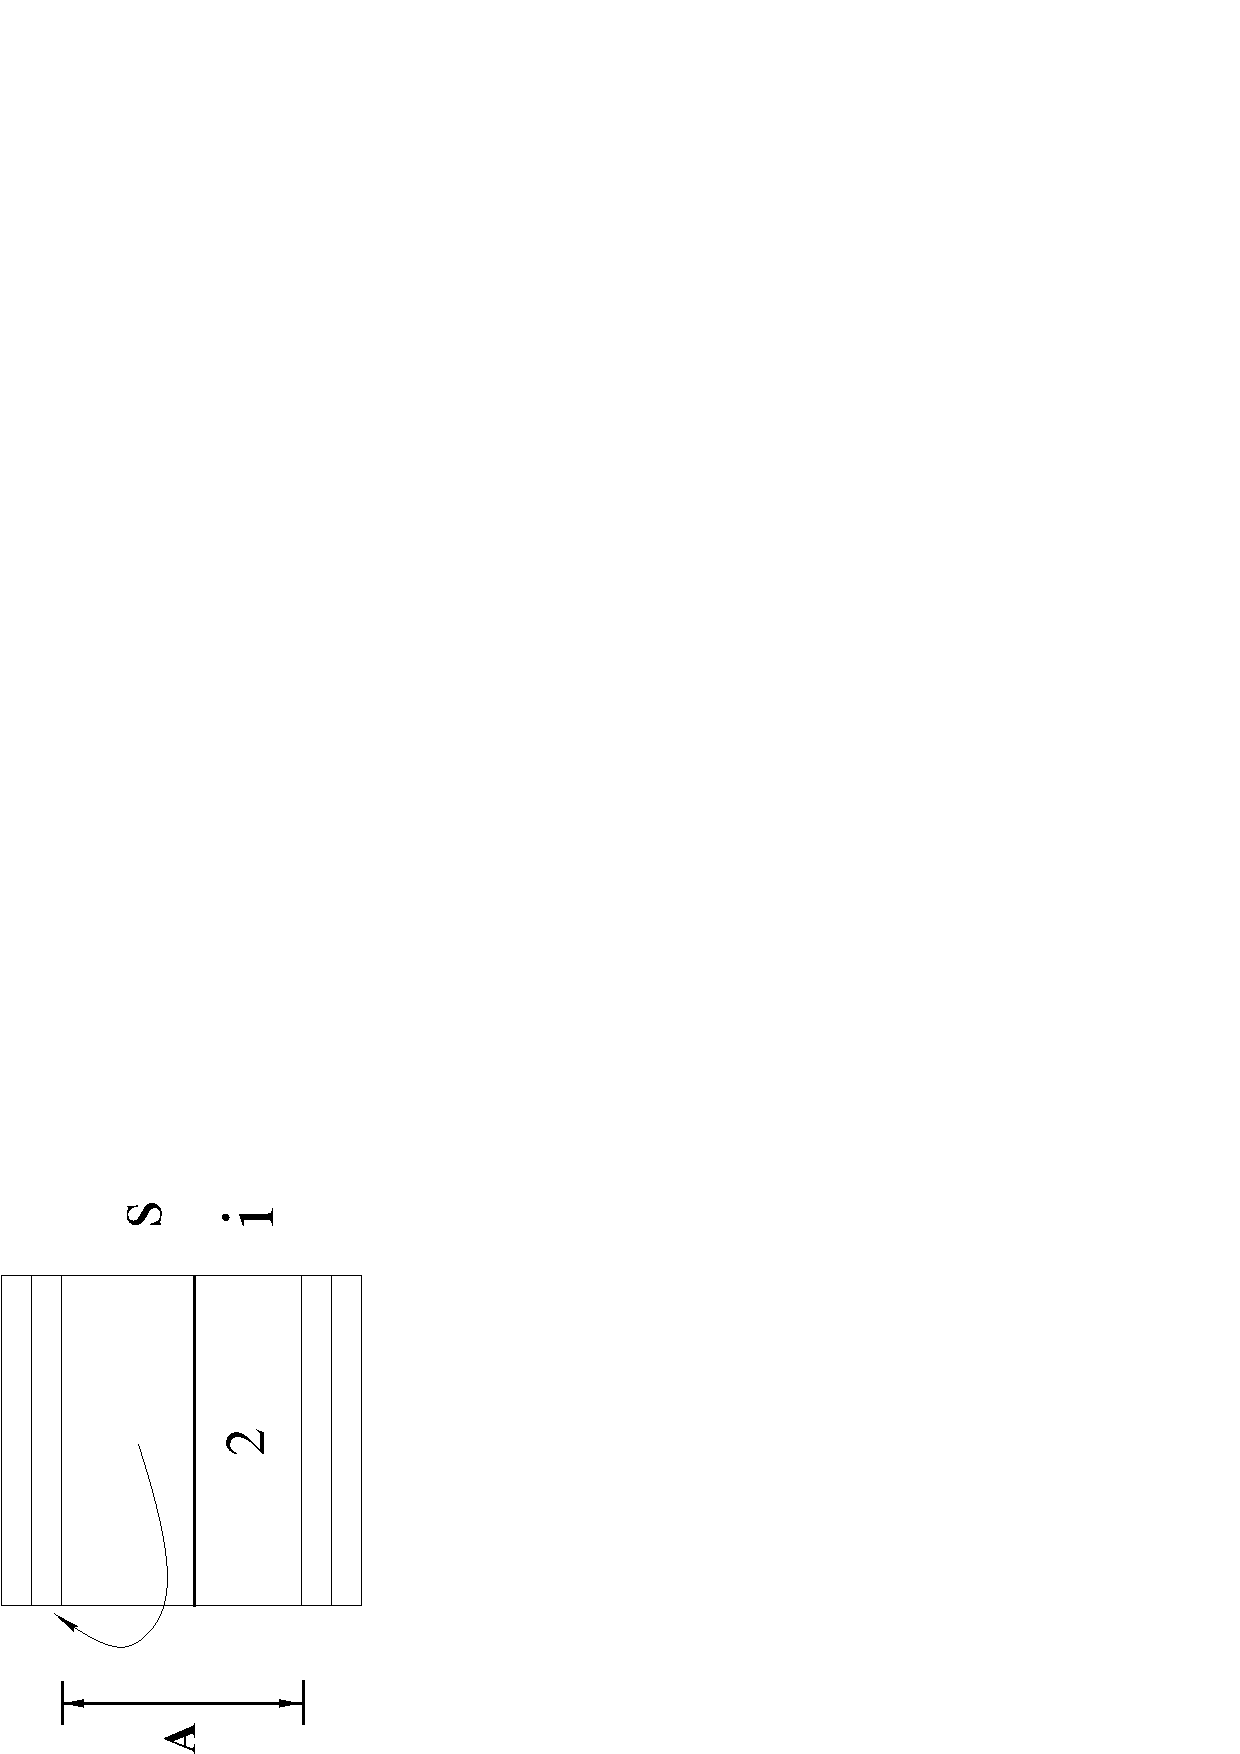
\includegraphics[angle=-90, scale=0.5]{hob1.pdf}}
\Caption{Skitse af hoben efter tildeling af {\tt A}'s felter.}
\label{f:hobfig1}
\end{figure}


\subsection{Variable}
Variable er enten variable defineret i metoder, eller er argumenter til metoder. Variablerne skabes hvergang metoden kaldes, og d�r, n�r metoden forlades. For begge typer variable g�lder det, at en s�dan opf�rsel elegant kan implementeres ved anvendelse af assemblers stak. Da et objekts felter gemmes i hoben istedet for p� stakken, er der ingen problemer med rekursive kald. For hvert rekursive kald, ligesom for alle andre metodekald, lagres argumenterne samt lokale variable f�rst p� stakken inden metodens indhold udf�res. Der er derfor ingen forskel p� metoder hvad entent de er rekursive i deres natur eller ej.


\begin{figure}[!h]
\centerline{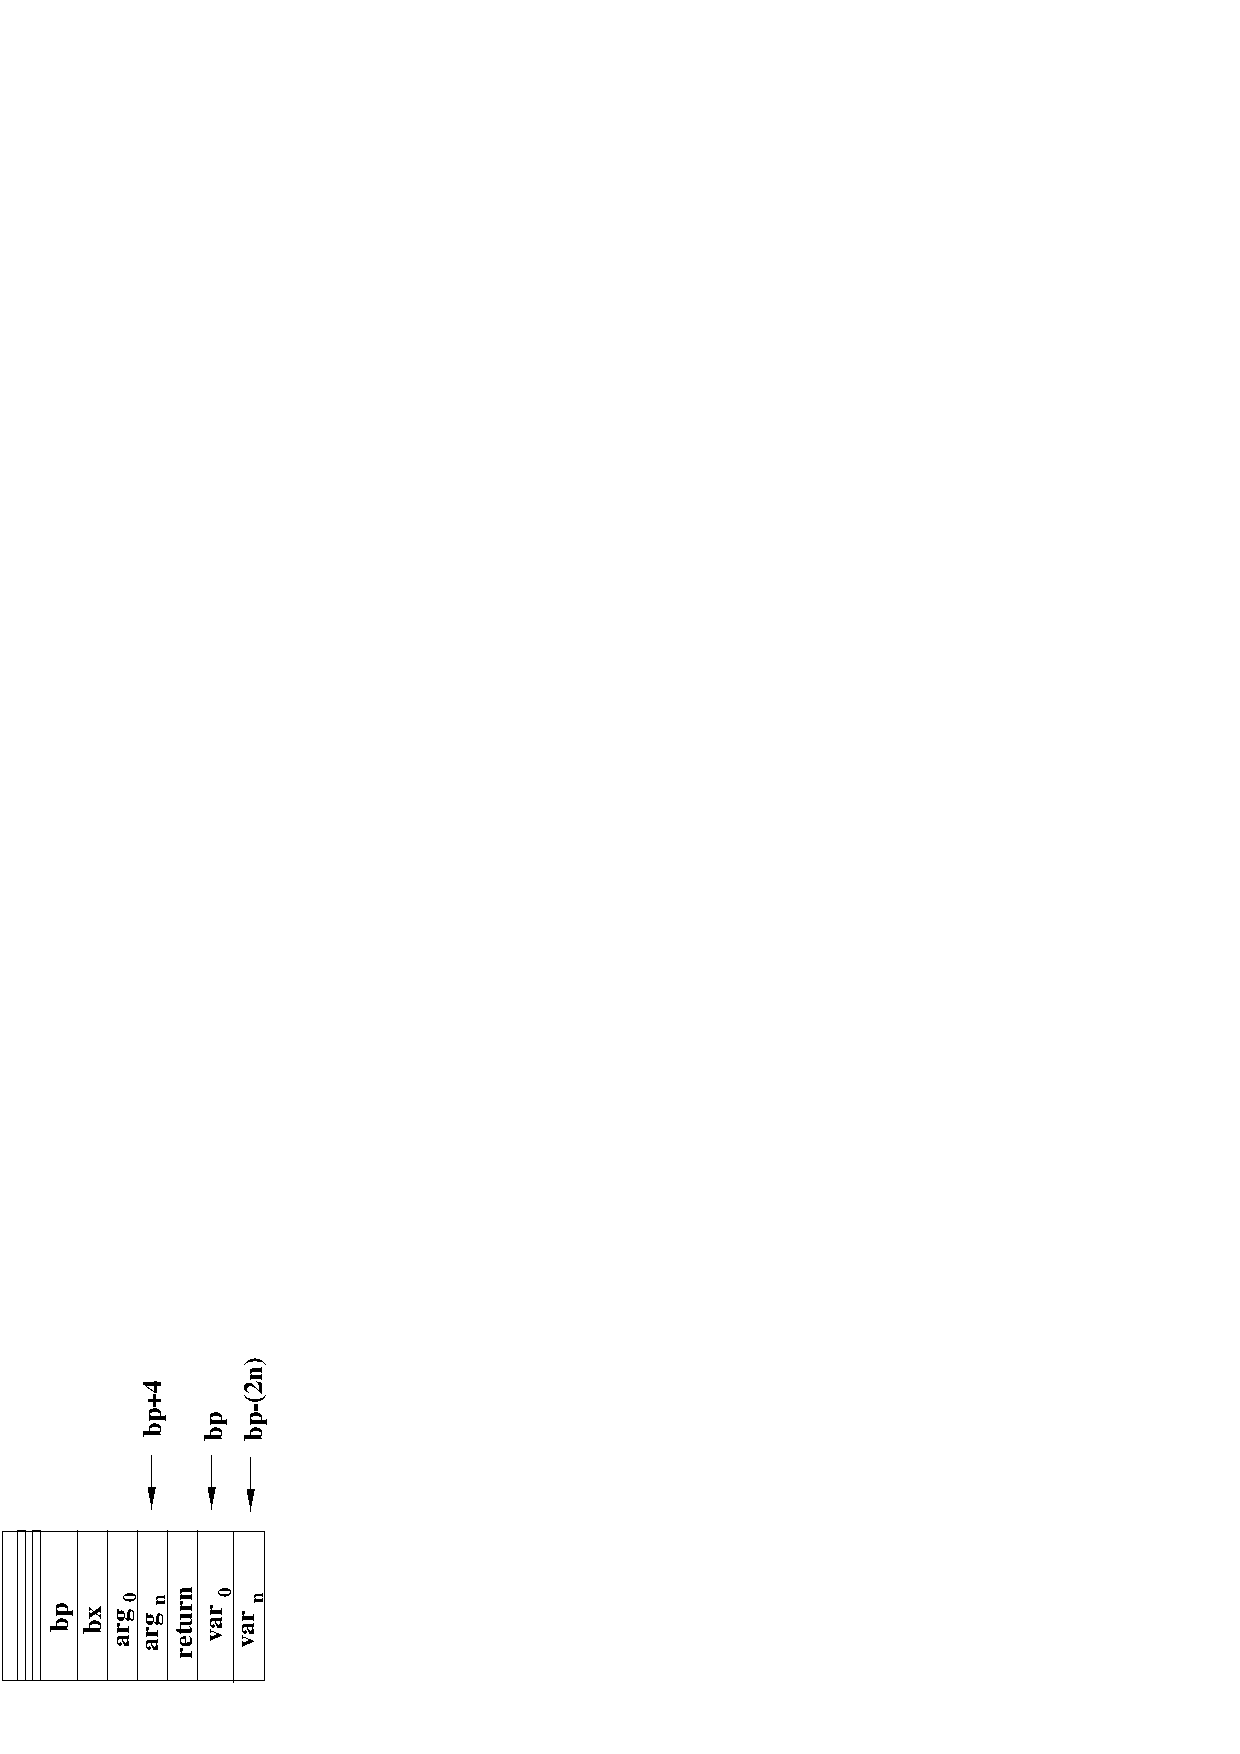
\includegraphics[angle=-90]{stak2.pdf}}
\Caption{Stakken som den tager sig ud lige efter et funktionskald.}
\label{f:stak1}
\end{figure}


\begin{quote}\example\begin{footnotesize}\begin{verbatim}
class B
{
    int b;
    
    void f(int x, int y)
    {
        int len;
        f(x, y);
    }
}
\end{verbatim}\end{footnotesize}\end{quote}

Stakkens udformning efter f�rste kald af \t{B.f()} ses p� \fref{f:stak1}. Registret \t{bp} peger altid p� den f�rste lokale variabel i metoden (p� stakken). Og da hver variabel fylder 16 bit, kan variablene tilg�s med \t{[bp-index]}, hvor \t{index} er variablens indexnummer. Indexnummeret tildeles variablene efter hvorn�r de defineres, s�ledes er den f�rste varibels index nummer = 0, men den n�ste er $2, 4, ...$. Argumenterne til metoden kan ligeledes tilg�s via \t{bp} registret, nemlig ved \t{[bp+4+index]}. De ekstra 4 adressepladser skyldes, at der skal hoppes forbi retur adressen. 

Ved brug af \t{bp} pointeren, er tilgangen til variable uafh�ngigt af hvor lidt eller hvor meget stakken anvendes.


\subsection{Felter}
Variable i klasse scope blev l�st og skrevet fra hoben. Styringen af hvor i hoben der l�ses og skrives styres af \t{bx} registret, der hele tiden indeholder `this' adressen for det aktuelle objekt. \t{bx} virker alts� som \t{this} referencen g�r i Java. Felter kan tilg�s p� to m�der, i det aktuelle objekt, eller fra andre objekter. For begge tilf�lde tilg�s variable med kaldet \t{hob[bx+index]}, hvor \t{index} er variablens index nummer. For felter i andre objekter skal man dog f�rst s�tte \t{bx} til det andet objekts `this' adresse. Dette g�res let, da det blot er referencevariablens v�rdi. Alts� for kaldet \t{a.i} udf�res:

\begin{quote} \example 
gem \t{bx};\\
bx = a;\\
\t{i} kan l�ses/skrives med \t{hob[bx+index]}\\
hent \t{bx};\\
\end{quote}

\subsection{Mellemresultater}
Da mellemresultater er tempor�re, og kun er anvendelige p� de konkrete steder, anbringes de p� stakken, hvor de automatisk fjernes (med \t{pop}), n�r de anvendes.


\subsection{Oprettelse af hoben}
For simpelthedens skyld, er hobens st�rrelse statisk og givet ved programmets start. Alle programmer der genereres indeholder s�ledes f�lgende blok kode, der allokerer hoben ved programstart. Koden er placeres i DATA-segmentet.

\begin{quote}\begin{footnotesize}\begin{verbatim}
hobptr  dw 0
hob     dw <HOBSIZE> dup(0)
\end{verbatim}\end{footnotesize}\end{quote}

Hvor \t{<HOBSIZE>} er en konstant indsat af compileren, der angiver hobens st�rrelse i antal word. Foruden hoben, allokeres ogs� en \t{hobptr}, en pointer, der angiver hvor meget af hoben der er i anvendelse, og som modificeres ved allokeringer. Da compileren ikke indeholder garbage collection, opbruges hoben med tiden, da ``d�de'' objekter, alts� objekter som ingen referencer har, ikke fjernes.


\begin{figure}[!h]
\centerline{\fbox{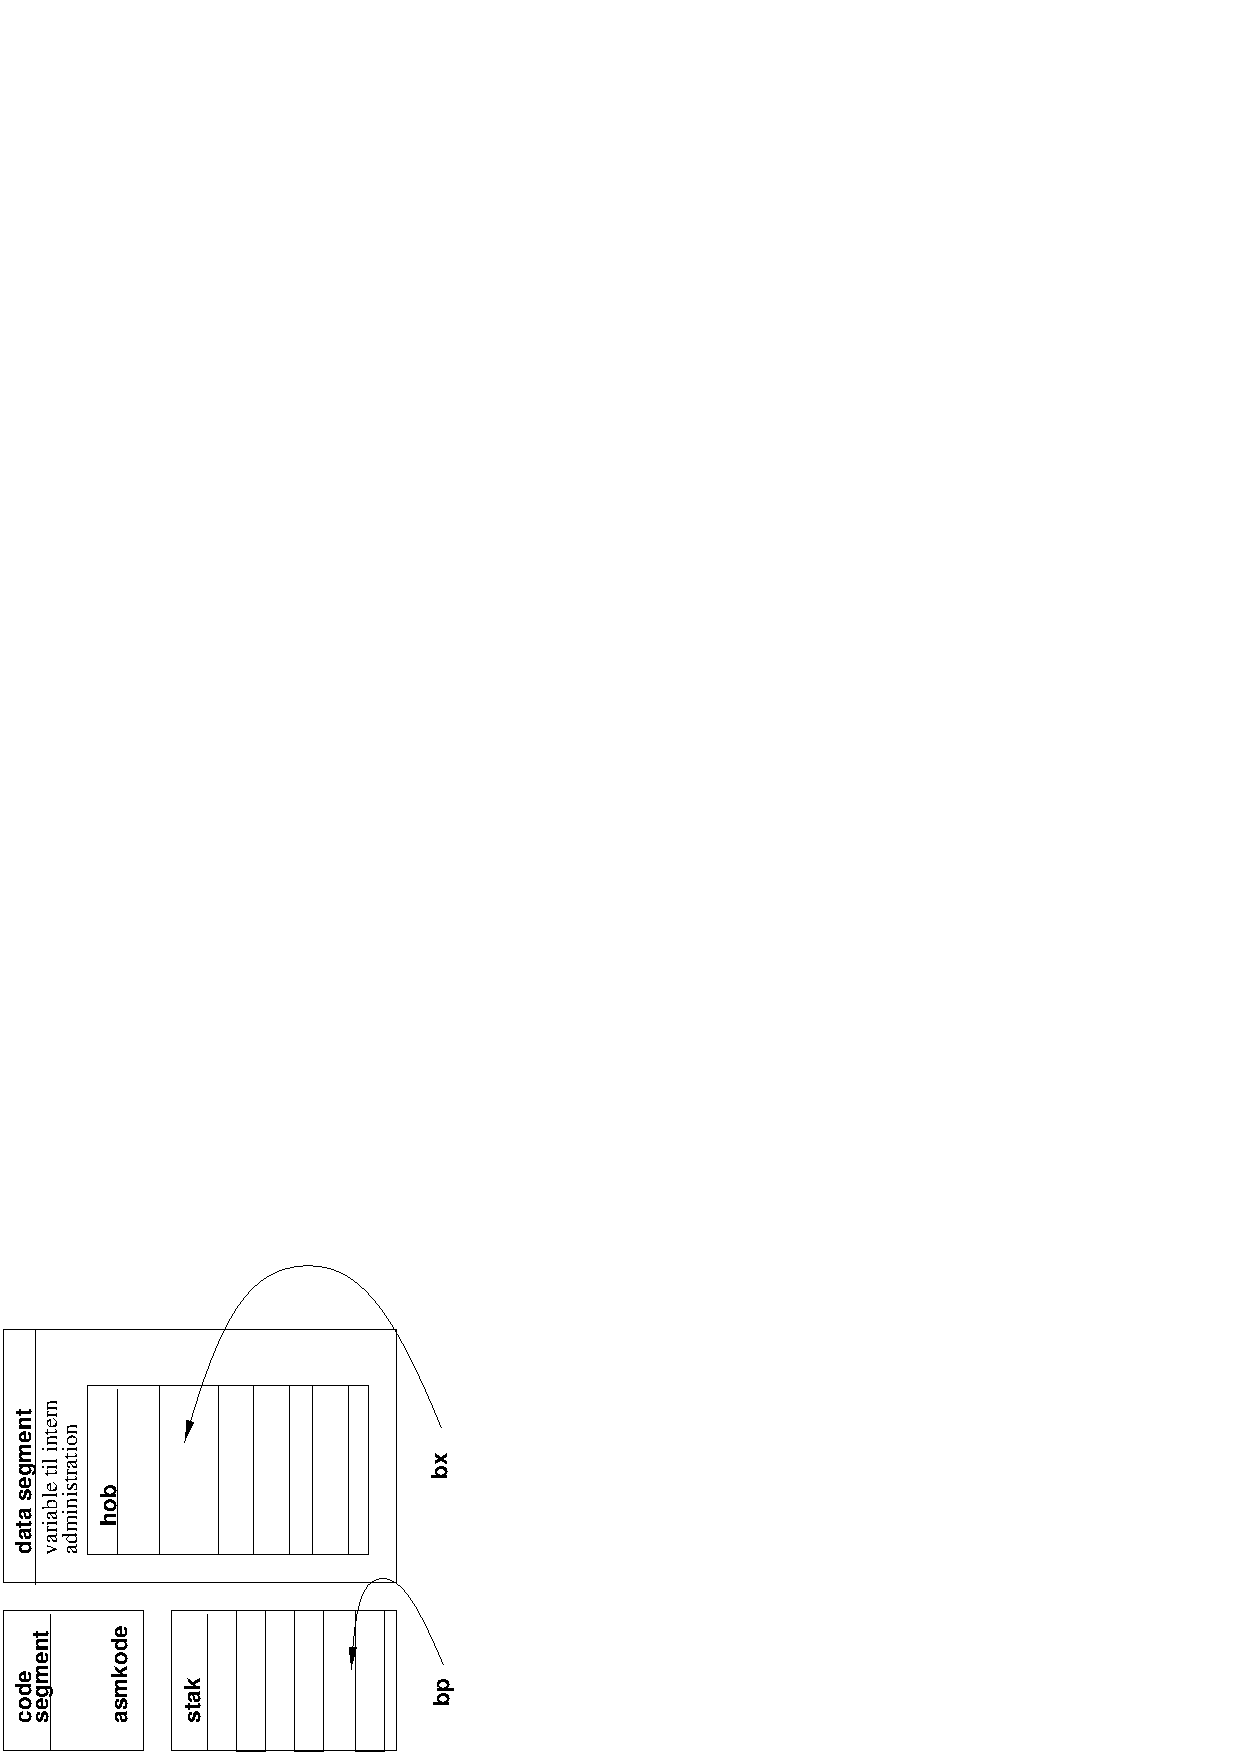
\includegraphics[angle=-90]{kodegenoversigt.pdf}}}
\Caption{Oversigt over lageradministrationen i Qjava.}
\label{f:kodeoversigt}
\end{figure}

\subsection{Opsummering}
Opsumeret p� \fref{f:kodeoversigt} er f�lgende gennemg�et
\begin{itemize}
\item[$\blacktriangleright$] Code segmentet indeholder den genererede assemblerkoden.
\item[$\blacktriangleright$] Data segmentet indeholder hoben, der rummer instanser af objekter samt interne variable til intern administration f.eks. hvor meget af hoben der er blevet anvendt.
\item[$\blacktriangleright$] Stakken anvendes til opbevaring af lokale variable samt argumenter til funktioner, som tilg�s \t{[bp-index]} og \t{[bp+4+index]}. 
\item[$\blacktriangleright$] Felter tilg�s med \t{hob[bx+index]}.
\end{itemize}

Der er alts� blevet forklaret, \textit{hvordan} hob, stak osv. tager sig ud. I de f�lgende sektioner, forklares \textit{hvorledes} henholdsvis stak, hob osv. f�r dette indhold.

\section{Referencer \& Objekter}
\label{s:referencerogobjekter}
Objekter ``allokeres'' med ved hj�lp af proceduren \t{new}. N�r \t{new} kaldes, reserveres et angivet antal bytes af hoben i en blok. Startadressen p� blokken returneres, mens \t{hobptr} t�lles op med st�rrelsen af den reserverede blok. 

Referencer til objekter har som alle andre variable en st�rrelse p� 16 bit. Men istedet for at indeholde en v�rdi, indeholder de adressen p� blokken der blev allokeret. F�lgende eksempel viser hvad der sker n�r koden \t{A a; (...) a = new A();} udf�res, og hvor klassen \t{A}'s st�rrelse er 4. V�rdien af \t{hobptr} ved start (i dette tilf�lde 30), er blot et udtryk for, at hoben ikke er tom p� tidspunktet eksemplet gennemg�s.

\begin{quote}\example
\textit{F�r allokering af A}\\
\t{~~~~hobptr == 30;} \\ 
\textit{Allokering af objekt med st�rrelse 4 bytes}\\ 
\t{~~~~gem hobptr;} \\ 
\t{~~~~hobptr = hobptr + 4;}\\ 
\t{~~~~return gammel hobptr;}\\
\t{~~~~a = retur-v�rdi;}
\end{quote}

Referencen til objektet f�r alts� v�rdien 30 (adressen p� hvor i hoben objektet befinder sig), mens \t{hobptr} har f�et v�rdien 34. N�r et ny objekt allokeres, bliver referencens v�rdi derfor 34.


\section{Metoder \& metodekald}
\label{s:metoderogmetodekald}
Metoder repr�senteres i assembler med procedurer. Da det vides, at klasse navne er unikke (sektion \xref{s:sprogdef}), kan metoderne navngives som \\
\verb�klassenavn_metodenavn�. Denne konstruktion g�r det let at generere assemblerkode, n�r et metodekald m�des.

Der findes to slags metodekald; Metodekald i eget objekt og metodekald i andre objekter . M�den de to tilf�lde h�ndteres p� er n�sten ens. I det f�lgende tages udgangspunkt i metodekald i andre objekter, som ogs� er skitseret p� \fref{f:stak1}. Den eneste forskel p� metodekald i eget og andre objekter er, at metodekald i eget objekt ikke genererer kode der �ndrer v�rdien af \t{bx} registret (this referencen for objektet).

\begin{itemize}
\item[$\blacktriangleright$] \t{bp} gemmes, da metoden definerer sin egen \t{bp}.
\item[$\blacktriangleright$] \t{bx} gemmes, da \t{bx} skal pege p� et andet objekt.
\item[$\blacktriangleright$] Assembler underst�tter ikke argumenter til procedurer, de push'es derfor p� stakken.
\item[$\blacktriangleright$] \t{bx} s�ttes til v�rdien af referencevariablen (der indeholder this adressen) og  \t{call} udf�res, hvilket medf�rer returadressen push'es.
\end{itemize}

I funktionen sker f�lgende
\begin{itemize}
\item[$\blacktriangleright$] \t{bp} s�ttes til \t{sp-2}, da dette er elementet efter retur-adressen p� stakken.
\item[$\blacktriangleright$] Antallet af lokale variable gange udf�res  \t{push 0}. De lokale variable initialiseres alts� til 0.
\end{itemize}

Lige f�r proceduren forlades udf�res

\begin{itemize}
\item[$\blacktriangleright$] Antallet af lokale variable gange udf�res \t{pop cx}.
\end{itemize}

Det �verste element p� stakken er returadressen, der hoppes til n�r \t{ret} m�des. Efter et metodekald, skal \t{bx, bp} gendannes, hvilket sker med:

\begin{itemize}
\item[$\blacktriangleright$] \t{pop bx, pop bp} udf�res for at genskabe ordnen i det gamle objekt s� det er i samme tilstand som f�r metodekaldet.
\end{itemize}



\section{Udtryk og s�tninger}
\label{s:udtrykogsaetninger}
S�tninger og udtryk opererer p� v�rdier p� stakken. Udtrykket \t{2+3} pop'er alts� 2 og 3 adderer dem og push'er resultatet. 


\subsection{Boolsk repr�sentation}
\label{ss:boolskrepraesentation}
M�den de boolske udtryk repr�senteres p� er \t{0000$\:$0000$\:$0000$\:$0000b} for false, og \t{1111$\:$1111$\:$1111$\:$1111b} for true, alts� henholdvis \t{0h} og \t{FFFFh}. Tallene er valgt udfra det faktum at assemblerkommandoerne \t{neg, and, or} fungerer uden videre. Var v�rdierne valgt som hhv. 0 og 1 (\t{0000$\:$0000$\:$0000$\:$0001b}), ville \t{neg} ikke fungere, da \t{neg 1} giver \t{FFFEh} (\t{1111$\:$1111$\:$1111$\:$1110b}) fremfor \t{0}.


\chapter{Kodegenerering}
\label{c:kodegenerering}
Dette kapitel tager udgangspunk i, at l�seren har forst�et det tidligere kapitel om specielt lageradministrationen og hvorledes klassers indhold bliver repr�senteret. Kapitlet skitserer hvorledes \t{CodeGenerator} genererer kode for de resterende dele af Qjava.


%\item Kodegenerering
% Standardfunktioner
% Opstarts og afslutningskode
% Implementation

\OverviewLineNoTitle



\section{Overordnet betragtning}
\label{s:kodegen_betragtning}

F�r den egenlige kodegenerering skal finde sted, kan det v�re fordelagtigt at illustrere rutediagrammer, der viser hvorledes strukturerede programmer tager sig ud. Figur \xref{f:rutediagram} viser ruterne programmer. \t{s} repr�senterer s�tninger, dvs. \i{sentences} i grammatikken, mens \t{E} repr�senterer udtryk, \i{E} i grammatikken.

Diagrammet til venstre p� figuren viser, at s�tninger genereres kronologisk, og individuelt uden hensyn til hverken foreg�ende eller kommende s�tninger. Dette g�lder for alle s�tninger i Qjava, med to undtagelser, nemlig s�tninger indeholdt i \t{if} og \t{while}.

Diagrammet i midten viser \t{if} der branch'er eller forgrener afviklingsforl�bet. Figuren viser, at evalueringen af \t{if} genereres selvst�ndigt, og der derfra hoppes til \t{s$_1$} eller \t{s$_2$}, der genereres som vist i det venstre rutediagram. Label \t{l} medtages da \t{s$_1$} efter endt generering skal hoppe til slutningen af \t{if}. Hvis dette hop ikke blev foretaget, ville kodeblokken \t{s$_2$} blive udf�rt.

Rutediagrammet til venstre viser \t{while}-l�kken. Koden \t{s$_1$} skal genereres sammen med informationen om navnet p� label \t{l}, til de tilf�lde hvor \t{break} m�des.


Det bem�rkes m�ske at metoder og klasser ikke er medtaget i rutediagrammerne. Grundene til dette er, for det f�rste er de meget sv�re at skitsere, og for det andet kan de betragtes ``indpakning af koden''. Det eneste der er interessant under kodegenereringen af en metode er, hvor metodens  argumenter og variable befinder sig, samt hvad navnet er p� en label placeret i bunden af metoden (som anvendet der hoppes til hvis \t{return} m�des. Bem�rk at viden om placeringen af metoden i en klasse, metodens funktionalitet osv. er fuldst�ndig underordnet. ``Indpakningen'' best�r s� og sige af lokale variable, argumenter samt en label. Klasser er det i kodegenerations sammenh�nge p� dette niveau kun, at \t{bx} registret indeholder this-referencen. \t{bx} administreres ved tilgang til variable i andre objekter og ved funktionskald til andre objekter.

\begin{figure}
\begin{center}
~~~\xymatrix@W=0.2cm@C=0.37cm
{
*\txt{s$_1$ ; s$_2$ ;} 		&								& *\txt{\t{if(E)}\{\ s$_1$\}\ \t{else} \{\ s$_2$\}}					&									& *\txt{\t{while(E)}\{\ s$_1$\}}\\
*++[o][F]{} \ar[d]			&								& *++[o][F]{}  \ar[d]												& 									& *++[o][F]{} \ar[d]\\
*++[o][F]{s_1} \ar[d]		&								& *++[F]{\txt{if E goto s$_1$ \\ else goto s$_2$}} \ar[ddr] \ar[dl]	&									& *++[F]{\txt{while E goto s$_1$}} \ar[d] \ar@/_3pc/[dd]\\
*++[o][F]{s_2} \ar[d]		& *++[o][F]{s_1} \ar@/_1pc/[dr]	&																	&  									& *++[o][F]{s_1} \ar@/_7pc/[u] \ar@/^3pc/[d]|{\txt{\t{break}}}\\
*++[o][F]{}					&								& *++[o][F]{l} \ar[d]												& *++[o][F]{s_2} \ar@/^1pc/[dl]		& *++[o][F]{l} \ar[d]	\\
							&                          		& *++[o][F]{}                                                       &                   		        & *++[o][F]{}\\                    
}
\end{center}
\Caption{Rutediagram for Qjava, hvor de tomme cirker noterer mulig eksistens af anden kode. s noterer s�tninger, E noterer udtryk og l noterer label der kan hoppes til.}
\label{f:rutediagram}
\end{figure}

\section{Kodegenerering}
Som det ses udfra skitseringen af syntaksen for assembler i sektion \xref{ss:asm_syntaks}, er det f�rste problem at omforme Java udtryk til noget der i de fleste tilf�lde har formen:  \mbox{\t{COMMANDO a$_1$ , a$_2$ }}. S�ledes bliver udtrykket \t{1-2-3} til

\begin{quote}
\t{t$_1$ = 1 - 2}\\
\t{t$_2$ = t$_1$ - 3}\\
\end{quote}

Omvendt er dette ikke et stort problem, da f.eks. alle udtryk allerede er p� denne form, i kraft af m�den de repr�senteres p� i parsertr�et. Kodegenereringen for ovenst�ende additionsudtryk vil derfor v�re \t{generer venstre tr�; generer h�jretr�}. Herefter vides det, at der findes to ``mellemresultater'' p� stakken. Der skrives ``mellemresultater'' da disse enten kan v�re tal, eller resultat af en anden beregning. Genereringen af venstretr�et vil v�re resultatet af genereringen af \t{1, -, 2}, som v�rende en mellemregning. Genereringen af h�jretr�et svarer til genereringen af \t{3}. De to ``mellemregninger'' pop'es fra stakken og subtraktionen udf�res, hvorefter resultatet push'es p� stakken.


\begin{center}
\mbox{
\xymatrix
{
          &                         & *+={-} \DOWNL \DOWNR \\
          & *+={-} \DOWNL \DOWNR    &                       & *+={3} \\
*+={1} 	  &                         & *+={2} \\
}}
\end{center}


bliver til

\begin{center}
\mbox{
\xymatrix
{
          & *+={-} \DOWNL \DOWNR     \\
*+={-1} 	  &                         & *+={3} \\
}}
\end{center}

der tilsidst bliver til $-4$


Kodegenereringen fra parsertr� til assemblerkode foreg�r udfra f�lgende to grundprincipper

\begin{itemize}
\item[$\blacktriangleright$] Givet en r�kke s�tninger ($1\dots n$), kan s�tningerne overs�ttes i kronologisk r�kkef�lge. Indholdet i hver s�tning, $0\dots n$ s�tninger/udtryk, overs�ttes p� samme vis kronologisk. 

\item[$\blacktriangleright$] Nettoeffekten af et udtryk, er pr�cis �n ekstra v�rdi p� stakken.
\end{itemize}

 Det skal bem�rkes, at f�rste regel skal forst�s rekursivt.
 

\subsection[Principperne i praksis]{Eksempel p� anvendelse af principperne}
\begin{quote}\example\begin{footnotesize}\begin{verbatim}
a = 2+3;

while(i < 100)
{
    i = i + 4+5;
    b = 6+7;
}
\end{verbatim}\end{footnotesize}\end{quote}

If�lge f�rste princip kan vi opsplitte overs�ttelsen i henholdsvis \\
~~~~\t{a = ...} og \t{while(...)\{...\}}.\\
\t{while} kan if�lge det andet princip opsplittes til:\\
~~~~\t{(...), \{...\}} , alts� en conditiondel og en krop,\\
hvor kroppen (\t{\{...\}}) kan opsplittes\\
~~~~\t{i = ...} og \t{b = ...}.\\
I alt 4 dele:

\begin{itemize}
\item[$\blacktriangleright$] \t{a = 2+3}
\item[$\blacktriangleright$] while condition: \t{i < 100}
\item[$\blacktriangleright$] while krop: \t{i = i + 4 + 5}
\item[$\blacktriangleright$] while krop: \t{b = 6+7}
\end{itemize}

Overs�ttelsen er skitsered p� \fref{f:asmgen}, hvor anden kolonne er d�t der skal overs�ttes, tredie kolonne skitserer kodegenereringen p� abstrakt plan, og sidste kolonne er et f�rs�g p� at skitsere hvorledes dette kunne tage sig ud i assembler. \# noterer et register. 
Linierne 2--7 viser, hvorledes mellemresultaterne 2 og 3 gemmes p� stakken. Additionsoperatoren pop'er de to �verste elementer, adderer og push'er resultatet (der evt. kunne v�re et mellemresultat, hvis udtrykket \t{2+3} havde v�re l�ngere. Det ses at resultatet af udtrykket var et ekstra element p� stakken, nemlig 5. Assign operatoren p� linierne 8--9 henter ogs� blindt v�rdierne der skal anvendes fra stakken. Eksemplet vil ikke blive yderligere forklaret, da principperne er tydeligt nok illustreret. 

For en god ordens skyld b�r det bem�rkes, at linierne 15--18 er en forsimpling af hvorledes kodegenereringen i Qjava fungerer. Forsimplingen er lavet for at bevare overblikket. Det der reelt sker i kodegenereringen er, at linierne 15--16 udf�res, men p� det der svarer til linie 16 hoppes ikke til \t{less}, men til et sted der push'er det boolske udtryk for true (\t{FFFFh}) og istedet for \t{jmp whileEndLabel} hoppes til et sted hvor der push'es det boolske udtryk for false (\t{0h}). F�rst herefter foretages en \t{push \#1, cmp \#1, 0} er \t{\#1} lig \t{FFFFh} (true) hoppes til label \t{less} ellers hoppes til label \t{whileEndLabel}.


\begin{figure}
\begin{center}
\begin{footnotesize}
\fbox{
\begin{tabular}{rlll}
Linie & Del		& Abstrakt	& pseudo assembler\\
\hline
1 & \t{a = 2+3}	& code(a =)	& \\
2 &				& code(2)	& \t{push 2}\\
3 &				& code(3)	& \t{push 3}\\
4 &				& code(ADD) & \t{pop \#1}\\
5 &				&			& \t{pop \#2}\\
6 &				&			& \t{add \#1, \#2}\\
7 &				&			& \t{push \#1}\\
8 &				&			& \t{pop \#1}\\
9 &				&           & \t{mov variable a, \#1 }\\
10&				&			& \t{start\underscore while:}\\
11&\t{i < 100}	& code(i)	& \t{push variable i}\\
12&				& code(100) & \t{push 100}\\
13&				& code(LESS)& \t{pop \#1}\\
14&				&			& \t{pop \#2}\\
15&				&			& \t{cmp \#1, \#2}\\
16&				&           & \t{jl less}\\
17&				&           & \t{jmp end\underscore while}\\
18&				&			& \t{less:}\\
19&\t{i = i+4+5}& code(i =) & \\
20&				& code(i)   & \t{push variable i}\\
20&				& code(4)   & \t{push 4}\\
. &				&			&\\
. & 			&			&\\
30&\t{b = 6 + 7}& code(b=)  &\\
31&				& code(6)   & \t{push 6}\\
. &				&			&\\
. &				&			&\\
40&				&			&\t{jmp start\underscore while} \\
41&				&           &\t{end\underscore while:} \\
\end{tabular}
}
\end{footnotesize}
\Caption{Figuren illustrerer hvorledes Java kan genereres til assembler.}
\label{f:asmgen}
\end{center}
\end{figure}



\subsection{Metoder og metodekald}
\label{ss:metoderogmetodekald}
Genereringen af metoder sker ved f�lgende: For hver metode (Fncdef) der m�des ved traversering af parsertr�et, dan f�lgende kode i code segmentet.

\begin{quote}\begin{footnotesize}\begin{verbatim}
klassenavn_metodenavn PROC

; her genereres metodens krop

klassenavn_metodensnavn ENDP
\end{verbatim}\end{footnotesize}\end{quote}

Metodekald genereres let. Givet koden \t{A a = new A();} og m�des udtrykket \t{a.f();} under traverseringen, genereres f�lgende kode: \verb�call typeVariablenHar_f� , hvor \t{typeVariablenHar} i dette tilf�lde er ``A'', som findes med en opslagsmetode i symboltabellen  Der genereres alts� \verb�call A_f�. Bem�rk administrationen af registrene \t{bp, bx} er fjernet fra eksemplet.

\section{Byggeklodser}
Som vist fra rutediagrammet og de efterf�lgende eksempler, er overs�ttelsen i mange tilf�lde blot at inds�tte ``byggeklodser'' for de forskellige slags udtryk og s�tninger sammen med en overordnet administration som beskrevet i det forrige kapitel. I de f�lgende undersektioner, gennemg�s assemblerkoden for byggeklodserne for s�tninger og udtryk. Da koden er meget simpel vil koden st� ukommenteret.

Generelt for implementationerne knytter sig nogle f� forholdsregler.

\begin{itemize}
\item[$\blacktriangleright$] De monadiske operatorer (\t{!, -}) forventer, at d�t de skal operere p�, forefindes �verst p� stakken. Implementationerne \t{pop}'er stakken, udf�rer operationen og \t{push}'er derefter resultatet.

\item[$\blacktriangleright$] De duale operatorer (de restende operatorer med undtagelse af \t{=}) forventer, at d�t de skal operere p�, forefindes �vers og n�st�verst p� stakken. Endvidere forventes det �verste element at repr�sentere h�jresiden af operatoren, n�r udtrykket skrives i sproget Qjava. Implementationerne \t{pop}'er de to �verste elementer fra stakken, udf�rer operationen og \t{push}'er derefter resultatet.

\item[$\blacktriangleright$] Specielt for operatorene \t{|, ||, \&, \&\&, <, <=, !=, ==} at disse ikke push'er en v�rdi, men et boolsk udtryk, som repr�senteres som henholdsvis \t{0h} og \t{FFFFh}. Videre begrundelse for dette findes i sektion \xref{ss:boolskrepraesentation}.


\item[$\blacktriangleright$] Generer kode til henholdsvis stak eller Hob tilgang beskrevet i de tidligere kapitler. \i{mem} (som forefindes i sektion \xref{ss:memdimsdut}) kan derfor v�re \t{hob[bx+index]} eller \t{bp-index}.
\end{itemize}

\twocolumn

\subsection{ \t{+}}
\begin{quote}\begin{footnotesize}\begin{verbatim}pop  dx
pop  ax
add  ax, dx
push ax
\end{verbatim}\end{footnotesize}\end{quote}


\subsection{ \t{-}}
\begin{quote}\begin{footnotesize}\begin{verbatim}pop  dx
pop  ax
sub  ax, dx
push ax
\end{verbatim}\end{footnotesize}\end{quote}


\subsection{ \t{-} (monadisk)}
\begin{quote}\begin{footnotesize}\begin{verbatim}pop  ax
neg  ax
push ax
\end{verbatim}\end{footnotesize}\end{quote}


\subsection{ \t{*}}
\begin{quote}\begin{footnotesize}\begin{verbatim}pop  dx
pop  ax
mul  dx
push ax
\end{verbatim}\end{footnotesize}\end{quote}


\subsection{ \t{/}}
\begin{quote}\begin{footnotesize}\begin{verbatim}pop  si
pop  ax
xor  dx, dx
div  si
push ax
\end{verbatim}\end{footnotesize}\end{quote}


\subsection{ \t{\%}}
\begin{quote}\begin{footnotesize}\begin{verbatim}pop  si
pop  ax
xor  dx, dx
div  si
push dx
\end{verbatim}\end{footnotesize}\end{quote}


\subsection{ \t{!}}
\begin{quote}\begin{footnotesize}\begin{verbatim}pop  ax
not  ax
push ax
\end{verbatim}\end{footnotesize}\end{quote}


\subsection{ \t{!=}}
\begin{quote}\begin{footnotesize}\begin{verbatim}pop  dx
pop  ax
cmp  ax, dx
jne  neq_1
xor  ax, ax    ; is ==
jmp  neq_end1
neq_1:
mov  ax, FFFFh ; is !=  true result
neq_end1:
push ax
\end{verbatim}\end{footnotesize}\end{quote}


\subsection{ \t{<=}}
\begin{quote}\begin{footnotesize}\begin{verbatim}
pop  dx
pop  ax
cmp  ax, dx
jle  lequal_1
xor  ax, ax    ; is not <=
jmp  lequal_end1
lequal_1:
mov  ax, FFFFh ; is <=  true result
lequal_end1:
push ax
\end{verbatim}\end{footnotesize}\end{quote}


\subsection{ \t{<}}
\begin{quote}\begin{footnotesize}\begin{verbatim}
pop  dx
pop  ax
cmp  ax, dx
jl   less_1);
xor  ax, ax    ; is not <
jmp  less_end1
less_1:
mov  ax, FFFFh ; is < // true result
less_end1:
push ax
\end{verbatim}\end{footnotesize}\end{quote}


\subsection{ \t{=}}
\label{ss:memdimsdut}
\begin{quote}\begin{footnotesize}\begin{verbatim}
pop ax
mov <MEM>, ax
\end{verbatim}\end{footnotesize}\end{quote}


\subsection{ \t{==}}
\begin{quote}\begin{footnotesize}\begin{verbatim}
; equal
pop  dx
pop  ax
cmp  ax, dx
je   eq_1
xor  ax, ax  ; is != // false result
jmp  eq_end1
eq_1:
mov  ax, FFFFh ; is == // true result
eq_end1:
push ax
\end{verbatim}\end{footnotesize}\end{quote}


\subsection{ \t{|, ||}}
\begin{quote}\begin{footnotesize}\begin{verbatim}
pop  dx
pop  ax
or   ax, dx
push ax
\end{verbatim}\end{footnotesize}\end{quote}


\subsection{ \t{\&, \&\&}}
\begin{quote}\begin{footnotesize}\begin{verbatim}
pop  dx
pop  ax
and  ax, dx
push ax
\end{verbatim}\end{footnotesize}\end{quote}



\subsection{\t{break}}
Hvis \t{break} kaldes udenfor en while l�kke meldes fejl ved compilering, ellers genereres:

\begin{quote}\begin{footnotesize}\begin{verbatim}
jmp while_end_label
\end{verbatim}\end{footnotesize}\end{quote}




\subsection{\t{return}}
Da \t{return} ikke returnerer v�rdier, hoppes til den sidste linie i assembler proceduren.

\begin{quote}\begin{footnotesize}\begin{verbatim}
jmp fnc_end_label
\end{verbatim}\end{footnotesize}\end{quote}


\onecolumn


\subsection{\t{if}}
\t{if} best�r af tre blokke henholdsvis\\
\t{if(condcode (1))\{thencode(2)\} else \{ elsecode (3)\}}. Da enten \t{thencode} eller \t{elsecode} skal udf�res skal der anvendes labels til at kunne hoppe til disse sektioner, endvidere skal der v�re label til i slutningen af \t{if} udtrykket (s� \t{thencode} ikke ogs� udf�rer \t{elsecode}), samt slutningen af funktionen skal kendes til \t{return}.

F�rst genereres condition koden (som princip 1 foreskriver) og evalueres. Resultat gemmes p� stakken som princip 2 foreskriver. Resultatet \t{pop}'es og evalueres og der udf�res hop til elsecode eller thencode alt efter resultatet. De to kodeblokke genereres som princip 1 foreskriver.

\begin{quote}\begin{footnotesize}\begin{verbatim}
; tree == the parsetree of instanceof If
; generate condition -> eGen(tree.getCond());
pop  cx
cmp  cx, 0  ; compare condition code
je   else1

then1:
; generate then code ->  sentenceGen(tree.getThen());
jmp  ifend1

else1:
; generate else code ->	sentenceGen(tree.getElse());

ifend1:
\end{verbatim}\end{footnotesize}\end{quote}


\subsection{ \t{while}}
\t{while} best�r af to blokke henholdsvis:\\
\t{while(condcode (1))\{whilecode (2)\}}. Til koden skal der endvidere produceres et ``startWhile'' og et ``slutWhile'' label.

\begin{quote}\begin{footnotesize}\begin{verbatim}
; tree == the parsetree of instanceof While
start_while1:
; generate condition code ->  sentenceGen(t.getCond());
pop  ax
cmp  ax, 0 ; compare condition code
je   end_while1

;generate while-body -> sentenceGen(tree.getWhile());
jmp  start_while1  ; loop once more

end_while1:
\end{verbatim}\end{footnotesize}\end{quote}




\section{Bootstrapping}
Funktionsdeklarationen \t{static void main()} erkl�rer starten p� et program. Qjava underst�tter ikke \t{static}, men ignorerer det af hensyn til kompabilitet med Java. N�r overs�tteren m�der funktionen \t{main()} (fra sektion \xref{s:sprogdef} er det givet der kun er en \t{main()} pr. program. Genereres en label ``START'' (i opstartskoden genereres kaldet \t{jmp START}). Herefter allokeres objektet funktionen befinder sig i (\t{<SIZEOFCLASS>} erstattes af klassens st�rrelse). Derefter justeres registrene \t{bp, bx}. Slutteligt genereres kroppen af main-funktionen.

\begin{quote}\begin{footnotesize}\begin{verbatim}
START:
    mov  cx, <SIZEOFCLASS>
    call new
    mov  bp, sp
    sub  bp, 2
    mov  bx, ax
    .
    .
\end{verbatim}\end{footnotesize}\end{quote}




\section{Standard funktioner}
\label{s:stdfunktioner}
Qjava implementerer dele af standardpakkerne der f�lger med Java. For \t{Integer, String} g�lder det, at de har overholdt samme navnekonventioner som dannelsen af andre funktioner, hvilket har den fordel at hvis \t{String s; s = "hej ib";} g�lder og udtrykket \t{s.length()} m�des, bliver \t{call}-kaldet genereret automatisk, som forklaret i eksemplet med \t{a.f()} kaldet i sektion \xref{ss:metoderogmetodekald}. 

Kodegenerering i forbindelse med metodekald til pakkerne \t{Integer, System} bliver h�ndteret individuelt for hver metode.

Da standardfunktionerne er simple, forklares deres implementation udelukkende. Der henvises derfor til slutningen af \aref{a:codegenerator} hvor implementationen er at finde.

\subsection{Integer}
Fra Integerpakken implementeres udelukkende metoden\\ \t{static String Integer.toString(int)} (klassen \t{Integer} implementeres ikke). Resultatet er internt, at en pointer til den dannede streng push'es p� stakken. Implementationen gennemg�r f�lgende faser i overs�ttelsen af et tal til en streng:

\begin{enumerate}
\item[$\blacktriangleright$] Er tallet negativt gemmes denne information og tallet multipliceres med $-1$.
\item[$\blacktriangleright$] S�l�nge tallet $> 0$; divider tallet med 10 og \t{push} resten ved divisionen, herved gemmes cifret l�ngst mod h�jre.
\item[$\blacktriangleright$] Alloker en ny \t{String} og fyld den vha. \t{pop}. 
\end{enumerate}

Ved anvendelse af stakken til tempor�r lagring af cifrene returneres cifrene i den omvendte og dermed korrekte r�kkef�lge.


\subsection{String}
String typen implementeres ved at v�re en klasse der indeholder et st�rrelsesfelt, der angiver l�ngden af strengen, mens resten af felterne indeholder tekststrengens respektive bogstaver. 


\t{String s = "blabla"} \begin{tabular}{|c|}
\hline L�ngde \\ \hline	\\T	\\e	\\g	\\n	\\	\\ \hline
\end{tabular}
\begin{tabular}{|c|}
\hline 6 \\ \hline b \\l \\a \\b \\l \\a \\ \hline
\end{tabular}

Da hvert tegn, samt st�rrelsesfeltet repr�senteres ved 16 bit, fylder tekststrengen ``Datamat!'' derfor $(8\cdot 2)+2$ bytes i hoben, n�r den repr�senteres i et \t{String} objekt. Referencer til \t{String} objekter peger p� det f�rste element i instansen, nemlig l�ngden af strengen, der for ``Datamat!'' er lig 8. Indexeringen af de enkelte bogstaver foreg�r som i Java ved at f�rste tegn ligger p� plads 0 og s� fremdeles.

Bem�rk at strengene ikke er 0-termineret. En strengs l�ngde bestemmes udelukkende ved st�rrelsesfeltet.

Foruden selve typen implementeres endvidere metoderne \t{concat(), length()} og \t{charAt()} der alle har samme funktionalitet som i Java.

\subsubsection{concat()}
\t{String concat(String)} funktionen fungerer ved at oprette en ny \t{String} med summen af de to \t{String} instanser (adderer f�rste element fra hver instans), hvorefter den nye streng fyldes med indholdet af de gamle strenge. 

Der kontrolleres ikke for om den ene eller begge referencer er \t{null}

\subsubsection{length()}
\t{int length()} l�ser st�rrelsesfeltet i instansen og returnerer denne. Der kontrolleres ikke hvorvidt referencen er \t{null}

\subsubsection{charAt()}
\t{char charAt(int)} returnerer ASCII v�rdien af den p�g�ldende possition. Da hvert bogstav fylder 2 bytes, og da instansen indeholder et st�rrelsesfelt, findes bogstavet i hoben ved 
\t{hob[bx+(possition*2)+2]}. Der kontrolleres ikke for ugyldige eller negative v�rdier af possitionen. Endvidere skal det bem�rkes at\ \t{System.out.print()} ikke kan udskrive typen char.

\subsection{System}
\subsubsection{System.exit}
\t{System.exit()} skal �jeblikkeligt stoppe afviklingen af programmet. Dette g�res med et DOS interupt kald.

\subsubsection{System.in.read}
Metoden l�ser et tegn fra tastaturet og er implementeret med et DOS interrupt kald.

\subsubsection{System.out.print}
Metoden udskriver et \t{String} instans til sk�rmen. Implementationen l�ser st�rrelsesfeltet og udskriver derefter tegnene et for et med et DOS interrupt kald.


\section{Registre}
De mange registre der findes i 80x86 har ikke alle samme funktionalitet. S�ledes kan visse registre anvendes til at referere til hukommelse mens andre ikke kan. Det er derfor ikke en tilf�ldighed at \t{bx} og \t{bp} registrene st�r for den overordnede administration. Nedenst�ende tabel viser i grove tr�k hvorledes registrene anvendes af compileren.

\medskip
\begin{tabular}{l|l}
Registre & Anvendelse \\
\hline
ab, cx, dx, si & Aritmetik og mellemresultater\\
bx, bp         & \t{this} pointer for klasser, funktioer og variable.\\
si, di         & Pointere relative offset, f.eks. bx\\
sp             & Indeholder adressen p� det �verste element p� stakken.\\
\end{tabular}


\section{Opstarts- og Afslutnings- kode}
Ligesom Java kr�ver en ``\t{static void main()}''-metode, kr�ver DOS en opstartskode f�r assemblerprogrammer kan afvikles.

\subsubsection{Opstartskode}
Opstartskoden fort�ller assembleren hvilken memorymodel der anvendes, hvor stor stakken skal v�re og hvor data-segmentet befinder sig i memory. Slutteligt hoppes til label ``START'', hvorfra kroppen af funktionen ``\t{static void main()}'' er placeret.

\begin{quote}\begin{footnotesize}\begin{verbatim}
DOSSEG
.MODEL SMALL
.STACK 200h

.DATA
    hobptr  dw 0
    hob     dw 32605 dup(0) ; allocate hob
    ; error messages
    oomstr	db	10,13,'Out of memory! Can not allocate another class.','$',0,0

.CODE
     mov ax, @data
     mov ds, ax
     jmp START
\end{verbatim}\end{footnotesize}\end{quote}



\subsubsection{Afslutningskode}
Pogrammer kan p� et hvilket som helst tidspunkt afsluttes med DOS interrupt 21 med argument \t{4ch}.

\begin{quote}\begin{footnotesize}\begin{verbatim}
    mov ah,4ch
    int 21h
\end{verbatim}\end{footnotesize}\end{quote}

Slutteligt kr�ver assembleren ordet ``\t{END}'' som sidste ord i sourcekoden.




\section{Implementation}
Udover implementeringen af standardfunktionerne, blev \t{CodeGenerator} implementeret ved en metode for hver knudetype der fandtes i parsertr�et. Den faste struktur var derfor klart en fordel, da alle felter var eksplicitte. Implementationen foregik da ogs� n�sten smertefrit, og �ndres strukturen i parsertr�et er det forholdsvis enkelt at g�re det samme i kodegeneratoren. Den eneste afvigelse fra parsertr�et er hvis \i{E$_{10}$} genkendes som en funktionskald, oprettes en \t{fncCall} knude, som sendes over i metoden \t{fncCallGen}, der genererer et funktionskald.


\chapter{K�rselsvejledning}
For at skabe en \t{*}.exe fil, der kan afvikles under DOS, skal man igennem flere stadier, denne korte vejledning vil vise hvilke og hvordan. Vejledningen tager udgangspunkt i et korrekt installeret Javamilj� (JDK) samt assemblermilj� (TASM).

\OverviewLineNoTitle

\subsubsection{.java $\longrightarrow$ .asm}
 F�rst skal  ens Java sourcekode compileres til assemblerkode, dette g�res ved at skrive

\verb�C:\>java Qjava filnavn�

 Dette afvikler Qjava compileren, der l�ser sourcekoden ``filnavn.java'', og skriver filen ``filnavn.asm''. Bem�rk, at der ingen endelse findes p� filen der gives som argument til compileren.

\subsubsection{.asm $\longrightarrow$ .exe}
Sidste stadie kr�ver b�de en assemblering og en linkning. Dette udf�res ved at skrive

\verb�C:\>tasm filnavn.asm�

\verb�C:\>tlink filnavn.obj�

Hvis alt har forl�bet problemfrit, findes nu ``filnavn.exe'', der kan afvikles.



\chapter{Afpr�vning}

\label{c:afprovning}
Dette kapitel vil vise test af compilerens enkelte dele samt tilsidst den f�rdige version. 

\begin{itemize}
\item[$\circlearrowright$] Lexer, sektion \xref{s:testlexer}.
\item[$\circlearrowright$] Parser , sektion \xref{s:testparser}.
\item[$\circlearrowright$] Symbol tabel , sektion \xref{s:testsymboltabel}.
\item[$\circlearrowright$] Kodegenerering, sektion \xref{s:testkodegenerering}.
\end{itemize}
\OverviewLine

Alle testk�rsler er, medmindre andet er noteret, udf�rt efter principperne ``ekstern testning''  der kort er beskrevet i \cite{hbhansen}. Testmetoden tager ikke udgangspunkt i programkoden, men i programkodens funktionalitet. Koden er alts� reduceret til en ``blackbox'', hvor det er transformationen fra input til output er i fokus. Der testes s�ledes for om basistilf�lde kendes, men ikke kombinationer imellem disse. Det vil sige, hvis programmet kan genkende tallet \t{42}, kan den ogs� genkende alle andre tal, og genkender den \t{1+2}, genkender den ogs� alle andre kombinationer af to tal og + operatoren.

I lexeren testes der for 1) kan alle keyword/operatorer genkendes, 2) kan strenge/tal genkendet,  og 3) seppereres ordene rigtigt.

Parseren testes med en, efter grammatikken syntatisk korrekt, program kode. Der testes alts� for  1) om parseren kan parse koden problemfrit, 2) om parseren genkender de korrekte produktioner og 3) om den tildeler prioriteterne for operatorene korrekt.

Symboltabellen testet for om dens metoder fungerer korrekt.

Afpr�vningsstrategien for kodegeneratoren er ikke en tilbundsg�ende unders�gelse af alle semantiske tilf�lde. M�let med testen er at se om der kan genereres fungerende kode for operatorer, standardfunktioner og basistilf�lde af grammatikkens s�tninger og udtryk. Afgr�nsningerne i afpr�vningen afbegr�nser dermed ogs� p�lideligheden af compileren til afgr�nsningen af afpr�vningen.


\section{Lexer}
\label{s:testlexer}
F�r selve testargumentationen fremf�res, forklares m�den testresultaterne er forelagt p�. I
Tabel \ref{t:test_lexResultater} er hver celle opdelt i to dele. ``\#'' noterer hvor mange tokens lexeren har genkendt, mens  ``Val'' angiver den hvad token blev genkendt som. I visse tilf�lde er der knyttet ekstra information til et token, disse informationer er placeret imellem ``()''.

Til afpr�vningen af klassen er tre forskellige testdata filer anvendt. Den f�rste testdata fil er opdelt i tre faser:


\begin{quote}\example\begin{footnotesize}\begin{verbatim}
/* Test datafil 1
 * for den lexikalske analyse...
 */

// F�rste fase - tegnsekvenser
, . ; : ( ) { } [ ]
+ - * / < % = != == <=
&& || & | ! break char class
else if int new null return
String void while

// Anden fase - v�rdi-test (char, tal og strenge)
'A' 12 "a str"

// Tredie fase - variabelnavn/separatorer test
foo2  2foo (foo foo( yif
ify 2int ((
a.b    c.d()    a. +
\end{verbatim}\end{footnotesize}\end{quote}


F�rste fase best�r i at genkende alle reserverede tegnsekvenser (hvis kommentarer genkendes ignoreres disse). Dette er Tokens 0--36 i tabel \ref{t:test_lexResultater}. Det bem�rkes at de to s�t kommentarer i starten af testfilen ikke har givet anledning til noget output, dvs. lexeren genkender kommentarer. Endvidere ses det at 1 og 2 returns samt 1 space betragtes som separator og ``whitespace'' hvorfor de ignoreres.

Anden fase best�r i v�rdi-genkendelse, alts� om lexeren forst�r tal, strenge og tegn. Dette er token 37--39. Det ses testdata blev genkendt som hhv. \t{A}, \t{12} og \t{Str val} som i testfilen.

Den sidste fase er en kombineret test af om variabelnavne kan genkendes, og hvad der er seperatorer. Token 40 viser, at tal i slutningen af en tegnsekvens ikke er en separator.  Token 41--42 viser, at tal er en sepperator, hvis det kommer f�rst i tegnsekvensen, dette ses ved tegnsekvensen opsplittes i to Tokens. Token 43--46 er en lignende test, hvor der istedet  anvendes en operator istedet for tal, i dette tilf�lde en ``\t{(}''. De to tegnsekvenser giver  fire tokens, hvorfor det konkluderes, at operatorer altid virker som sepperatorer. Token 46--47 viser, at lexeren genkender den l�ngst mulige tegnsekvens, da \t{if}-delen i begge tegnsekvenser ikke resulterede i et \t{if}-token. Token 49--50 viser tal og keywords separeres korrekt. Token 51--52 viser dobbelt operator virker, 53--54 viser genkendelsen af \i{name}, mens 26, 30, 34, 57 viser genkendelsen af \i{id}.

\begin{table}[!h]
\begin{center}
\begin{tabular}{|rl|rl|rl|rl|}
\hline
\# & Val & \# & Val & \# & Val & \# & Val \\
\hline
0 & , & 1 & . & 2 & ; & 3 & :\\ \hline
4 & ( & 5 & ) & 6 & \{ & 7 & \}\\ \hline
8 & [ & 9 & ] & 10 & $+$ & 11 & $-$\\ \hline
12 & * & 13 & / & 14 & $<$ & 15 & \%\\ \hline
16 & = & 17 & != & 18 & == & 19 & <=\\ \hline
20 & \&\& & 21 & $||$ & 22 & \& & 23 & $|$\\ \hline
24 & ! & 25 & break & 26 & id (char) & 27 & class\\ \hline
28 & else & 29 & if & 30 & id (int) & 31 & new\\ \hline
32 & null & 33 & return & 34 & id (String) & 35 & void\\ \hline
36 & while & 37 & chVal('A') & 38 & intVal(12) & 39 & StrVal(a str)\\ \hline
40 & id (foo2) & 41 & intVal(2) & 42 & id (foo) & 43 & (\\ \hline
44 & id (foo) & 45 & id (foo) & 46 & ( & 47 & id (yif)\\ \hline
48 & id (ify) & 49 & intVal(2) & 50 & id (int) & 51 & (\\ \hline
52 & ( & 53 & name (a.b) & 54 & name (c.d) & 55 & (\\ \hline
56 & ) & 57 & id (a.) & 58 & $+$ & 59 & <EOF>\\ \hline
\end{tabular}\end{center}
\Caption{Testudskrift for klassen {\tt Lexer}.}
\label{t:test_lexResultater}
\end{table}


\subsubsection{Testk�rsel 2}
Resultatet af testk�rsel 2 er:\\
\t{Error(1): Char definition more than 1 character long.}

\subsubsection{Testk�rsel 3}
Resultatet af testk�rsel 3 er:\\
\t{Error(1): keyword "switch" is not yet supported.}

For begge testk�rsler g�lder det, at compileren stoppede k�rslen efter udskrift.


\begin{quote}\example\begin{footnotesize}\begin{verbatim}
/* 2. testfil */
'aa'
\end{verbatim}\end{footnotesize}\end{quote}


\begin{quote}\example\begin{footnotesize}\begin{verbatim}
/* 3. testfil */
switch i;
\end{verbatim}\end{footnotesize}\end{quote}



\subsection{Ikke-problematiske fejl}
En fejl den anvendte testmetode ikke fangede er tilf�lde s�som \t{<\showspace =} Alts� hvor de to tokens klart er separeret af en space (\showspace ). Lexeren overs�tter dog det angive eksempel til et \t{<=} token. For implementationen af compileren er dette ikke noget problem da det ikke strider imod principperne for fejlmelding i kravsspecifikationen. Endvidere tillader Javasyntaxen ikke en s�dan konstruktion. Slutteligt kunne man med rette h�vde, at skriver man \t{<\showspace =} mener man faktisk \t{<=}.

Forklaringen p� opf�rslen finder vi i koden, hvor der her kun vises de for problemstillingen v�senligste dele (for en fuld kodeudskrift af lexerens testkode henvises til \aref{a:lexer}. \t{fetchOperator()} bliver kaldt i de situationer hvor Lexeren har l�st et ``\t{<}'' --- alts� situationer hvor der muligvis er tale om et sammensat token.


\begin{quote}\example\begin{footnotesize}\begin{verbatim}
class Lex extends StreamTokenizer implements TokenNames
{
...
  private Token fetchOperator(char c) throws IOException
  {
    int nt = super.nextToken();
...
    String s = "" + c + (char) nt;
...
    if(s.equals("<=")) return( new Token(LEQUAL) );
...
\end{verbatim}\end{footnotesize}\end{quote}

Som det ses, er det \t{StreamTokenizer} der st�r for indl�sningen, og da denne 1) ignorerer spaces 2) stopper og returnerer for hver operator, har man ingen mulighed for at vide om \t{StreamTokenizer}'en har m�dt \t{<\showspace =} eller \t{<=} konstruktionen.

Da der i forhold til kravsspecifikationen ikke opst�r vanskeligheder, uddybes problemstillingen ikke videre.



\section{Parser}
\label{s:testparser}
Testen af parseren tager udgangspunkt i f�lgende testfil,

\begin{quote}\example\begin{footnotesize}\begin{verbatim}
/*
 * test for parseren 23.11.99
 */

class A
{
    int i;// vardef i classscope
    ;
    void a() // fncdef uden argumenter
    {
        a(); // fnccall til eget og andre objekter
        b(1, 2,3);
        B.c();

        if(a) // if
        {
            aaa = 2; // assign
        }
        else
        {
            B.j = 3; // assign i andet objekt
        }
    }



    void b(int k, String l) // fncdef med argumenter
    {
        break;
        return;

        while(i != 2) // en while
        {
            return(); // return med parenteser
        }

        ; // tom linie (kun ";")
    }
}


// multible klasser
class B
{
    void c()
    {
        // vardef i function scope
        int j;
        int k;

        // E-E11     testes
        e = 1 || 2;
        e1 = 3 && 4;
        e2 = 5 | 6;
        e3 = 7 & 8;
        e4_1 = 9 == 10;
        e4_2 = 11 != 12;
        e5_1 = 13 < 14;
        e5_2 = 15 <= 16;
        e6_1 = 17 + 18;
        e6_2 = 19 - 20;
        e7_1 = 21 * 22;
        e7_2 = 23 / 24;
        e7_3 = 25 % 26;

        e8 = new B();
        e9_1 = !27;
        e9_2 = -28;
        e10_1 = foo;
        e10_2 = foo.bar;
        e10_3 = foo(29+30);
        e10_4 = foo(31, 32);
        e10_5 = "en streng";
        e11_1 = 2;
        e11_2 = (3);

        // en kombinations af flere E'er
        if( (a != 2 && b == 3) || (c < -2|3) || !(d <= e&4%5*6+7- -8/9) )
        {
            int x;
        }
        else
        {
        }

        i = 2+3*4;
        i = (2+3)*4;
        i = 2-3-4;
    }
}
\end{verbatim}\end{footnotesize}\end{quote}

For at kunne vurdere resultaterne, fort�ller parseren hvorledes den opfatter et givent udtryk, f.eks. med \t{(assign)}. Endvidere s�ttes parenteser om alle monadiske og duale operatorer for at kunne vise prioriteten i evalueringsr�kkef�lgen. For l�sbarhedens skyld, er testoutput modificeret med ekstra indrykninger og tilpasning af linieskift.

Gennemgangen af afpr�vningen foreg�r, af hensyn til overblikket, udfra grammatikken p� \fref{t:samletGrammar}, istedet for en kronologisk opremsning af eksemplet. Der henvises i�vrigt til hele \kref{c:qjavaspecifikation} for gennemgangen af grammatikken. I gennemgangen vises det, at hver non-terminal eksisterer i eksemplet, og at alle definitionerne p� non-terminalen eksisterer (f.eks. kan \i{sentece} repr�senteres ved b�de \i{while} og \i{fnccall} osv). Argumentationsformen er meget kompakt i den forstand, at non-terminalen opskrives, hvorefter beviset for at non-terminalen eksisterer, og at alle definitioner er afpr�vet. Non-terminalens definition gennemg�s ikke, da en s�dan gennemgang er at finde i kapitel \ref{c:qjavaspecifikation}.

\begin{itemize}
\item[\i{S}] Eksemplet indeholder klasserne \t{A}, \t{B}.
\item[\i{classdef}] Klassen \t{A} d�kker definitionen.
\item[\i{classcontents}] \t{A.i} opfylder \i{vardef}, \t{A.a()} opfylder \i{fncdef} og ``\t{;}'' forefindes i klasse scope i \t{A}.
\item[\i{vardef}] Variablen \t{A.i} opfylder \i{vardef}
\item[\i{fncdef}] Funktionerne \t{A.a()}, \t{A.b()} defineres hhv. uden og med argumenter.
\item[\i{sentences}] \i{vardef}, \i{fnccall}, ... , ``\t{;}'' forefindes i eksemplet.
\item[\i{fnccall}] �verst i \t{A.a()} repr�senterer \t{a()}, \t{B.c()} hhv. \i{id} og  \i{name}. kombinationen. \t{b(1, 2,3);} viser, der accepteres multible argumenter.
\item[\i{if}] \t{if(a)...} i \t{A.a()} og \t{if( (a != 2...)} nederst i \t{B.c()} viser \t{if} med og uden \t{else}-krop.
\item[\i{while}] Eksisterer i \t{A.b()}.
\item[\i{break}] Findes i \t{A.b();}.
\item[\i{return}] Findes med og uden \t{()} i \t{A.b()}.
\item[\i{assign}] Variablen \t{aaa} tildeles i \t{A.a()}.
\item[\i{E}-\i{E$_{11}$}] Er repr�senteret i \t{B.c()}
\end{itemize}

Resultatet viser de to n�stsidste tildelingss�tninger (\t{2+3*4}) i eksemplet, at prioriteten for evaluering kan �ndres ved hj�lp af parenteser. Den sidste tildelingss�tning (\t{2-3-4}) viser, at udtryk med flere operatore med ens prioritet, placeres korrekt i parsertr�et. Slutteligt er det lange sammensatte if-udtryk medtaget for at vise, at operatorene kan sammens�ttes uden problemer.
\begin{quote}\begin{footnotesize}\begin{verbatim}
class A
{
    (vardef) int i

    (fncdef) void a()
    {
        (fnccall) a()
        (fnccall) b(1, 2, 3)
        (fnccall) B.c()
        if(a)
        {
            (assign) aaa = 2
        }
        else
        {
            (assign) B.j = 3
        }
    }

    (fncdef) void b(int k, String l)
    {
        break
        return
        while((i != 2))
        {
            return
        }
    }
}

class B
{
    (fncdef) void c()
    {
        (vardef) int j
        (vardef) int k
        (assign) e = (1 || 2)
        (assign) e1 = (3 && 4)
        (assign) e2 = (5 | 6)
        (assign) e3 = (7 & 8)
        (assign) e4_1 = (9 == 10)
        (assign) e4_2 = (11 != 12)
        (assign) e5_1 = (13 < 14)
        (assign) e5_2 = (15 <= 16)
        (assign) e6_1 = (17 + 18)
        (assign) e6_2 = (19 - 20)
        (assign) e7_1 = (21 * 22)
        (assign) e7_2 = (23 / 24)
        (assign) e7_3 = (25 % 26)
        (assign) e8 = new B()
        (assign) e9_1 = (! 27)
        (assign) e9_2 = (- 28)
        (assign) e10_1 = foo
        (assign) e10_2 = foo.bar
        (assign) e10_3 = foo((29 + 30))
        (assign) e10_4 = foo(31, 32)
        (assign) e10_5 = "en streng"
        (assign) e11_1 = 2
        (assign) e11_2 = 3
        if(((((a != 2) && (b == 3)) || ((c < (- 2)) | 3)) ||
        (! ((d <= e) & ((((4 % 5) * 6) + 7)         - ((- 8) / 9))))))
        {
            (vardef) int x
        }
        else
        {
        }

        (assign) i = (2 + (3 * 4))
        (assign) i = ((2 + 3) * 4)
        (assign) i = ((2 - 3) - 4)
    }
}
\end{verbatim}\end{footnotesize}\end{quote}



\section{SymbolTable}
\label{s:testsymboltabel}
Med udgangpunkt i eksemplet i sektion \ref{s:testparser}, afpr�ves symboltabellen.

Efter endt parsing udf�res f�lgende kode, hvor \t{sbtb} er \t{SymbolTable}, alts� symboltabellen.

\begin{quote}\begin{footnotesize}\begin{verbatim}
System.out.println("1. A = "         + sbtb.classSize("A"));
System.out.println("2. B = "         + sbtb.classSize("B"));
System.out.println("3. B.c() = "     + sbtb.fncSize("B","c"));
System.out.println("4. B.c().x = "   + sbtb.varIndex("B","c","x"));
System.out.println("5. B.k = "       + sbtb.varIndex("B", null, "k"));
System.out.println("6. vartype i = " + sbtb.varType("A", "a", "i"));
sbtb.add("char", "A", null, "c", 42);
System.out.println("7. A.c = "       + sbtb.varIndex("A", null, "c"));
\end{verbatim}\end{footnotesize}\end{quote}

Hvilket gav f�lgende output

\begin{quote}\begin{footnotesize}\begin{verbatim}
1. A = 2
2. B = 0
3. B.c() = 6
4. B.c().x = 4
5. B.k = -1
6. vartype i = int
7. A.c = 42
\end{verbatim}\end{footnotesize}\end{quote}

Forklaringen af linierne:
\begin{enumerate}
\item \t{A} indeholder \t{i} == 2 bytes.
\item \t{B} indeholder ingen felter.
\item Variablen \t{x} er defineret som den tredie variabel i scope'et \t{B.c()} og f�r indexv�rdien 4 (variable indexeres 0, 2, 4, 6, ...). Det bem�rkes, at selvom \t{x} befinder sig i et \t{if}-scope, anvendes det i compileren som v�rende erkl�ret i \t{B.c()}'s scope.
\item Variablen \t{k} findes ikke i \t{B}'s klasse scope.
\item Der returneres den rigtige type, da \t{i} erkl�res som \t{int}.
\item Metoden \t{SymbolTable.add()}, hvor index nummeret selv kan fasts�ttes virker.
\end{enumerate}


\section{CodeGenerator}
\label{s:testkodegenerering}
\begin{quote}\begin{footnotesize}\begin{verbatim}
class A
{
    String space;
    String strfalse;
    String strtrue;

    void f()
    {
        int i;
        int j;

        // 00000000 00000100 (4) OR 00000000 00000010 (2) = 00000000 00000110 (6)
        System.out.print( Integer.toString(4|2) );  // | test
        System.out.print(space);

        // 00000000 00001100 (12) AND 00000000 00001010 (10) = 00000000 00001000 (8)
        System.out.print( Integer.toString(12&10) );// & test
        System.out.print(space);

        System.out.print( Integer.toString(1+1) );  // + test (2)
        System.out.print( Integer.toString(4-1) );  // - test (3)
        System.out.print( Integer.toString(2*3) );  // * test (6)
        System.out.print( Integer.toString(25/5) ); // / test (5)
        System.out.print( Integer.toString(23%8) ); // % test (7)
        System.out.print( Integer.toString(6- -2) );// - (fortegn) test (8)
        System.out.print(space);


        // ! test p� bits 11111111 11111000 (65528) = 00000000 00000111 (7)
        System.out.print( Integer.toString(!65528) );
        System.out.print(space);
        System.out.print(space);



        // == test 1
        j = 1;
        if(j == 1){System.out.print(strtrue);}
        else{System.out.print(strfalse);}

        // == test 2
        j = 0;
        if(j == 1){System.out.print(strtrue);}
        else{System.out.print(strfalse);}
        System.out.print(space);
        System.out.print(space);

        // != test 1
        j = 0;
        if(j != 1){System.out.print(strtrue);}
        else{System.out.print(strfalse);}


        // != test 2
        j = 1;
        if(j != 1){System.out.print(strtrue);}
        else{System.out.print(strfalse);}
        System.out.print(space);
        System.out.print(space);


        // < test 1
        j = 0;
        if(j < 1){System.out.print(strtrue);}
        else{System.out.print(strfalse);}

        // < test 2
        j = 1;
        if(j < 1){System.out.print(strtrue);}
        else{System.out.print(strfalse);}
        System.out.print(space);
        System.out.print(space);


        // <= test 1
        j = 0;
        if(j <= 1){System.out.print(strtrue);}
        else{System.out.print(strfalse);}


        // <= test 2
        j = 1;
        if(j <= 1){System.out.print(strtrue);}
        else{System.out.print(strfalse);}


        // <= test 3
        j = 2;
        if(j <= 1){System.out.print(strtrue);}
        else{System.out.print(strfalse);}
        System.out.print(space);
        System.out.print(space);


        // ! test p� boolske udtryk 1, false
        if(!(1 == 1)){System.out.print(strtrue);}
        else{System.out.print(strfalse);}


        // ! test p� boolske udtryk 2, false
        if(!(1 == 0)){System.out.print(strtrue);}
        else{System.out.print(strfalse);}
        System.out.print(space);
        System.out.print(space);



        // && test 1
        j = 0;
        if(j == 1 && j == 0){System.out.print(strtrue);}
        else{System.out.print(strfalse);}


        // && test 2
        j = 0;
        if(j == 1 && j == 1){System.out.print(strtrue);}
        else{System.out.print(strfalse);}


        // && test 3
        j = 0;
        if(j == 0 && j == 0){System.out.print(strtrue);}
        else{System.out.print(strfalse);}
        System.out.print(space);
        System.out.print(space);



        // || test 1
        j = 0;
        if(j == 1 || j == 0){System.out.print(strtrue);}
        else{System.out.print(strfalse);}


        // || test 2
        j = 0;
        if(j == 1 || j == 1){System.out.print(strtrue);}
        else{System.out.print(strfalse);}


        // || test 3
        j = 0;
        if(j == 0 || j == 0){System.out.print(strtrue);}
        else{System.out.print(strfalse);}
        System.out.print(space);
        System.out.print(space);



        // while test, udskriver 0
        j = 0;
        while(j == 0)
        {
            System.out.print( Integer.toString(j));
            j = j + 1;
        }


        // while test, udskriver intet
        j = 6;
        while(j < 5)
        {
            System.out.print( Integer.toString(j));
            j = j + 1;
        }
        System.out.print(space);


        // while test, udskriver 1..5
        j = 0;
        while(j < 5)
        {
            System.out.print( Integer.toString(j));
            j = j + 1;
        }
        System.out.print(space);
        System.out.print(space);


        // test af break, udskriver intet
        j = 0;
        while(j < 5)
        {
            break;
            System.out.print( Integer.toString(j));
        }


        // test af return, udskriver ikke mere
        return;
        j = 42;
        System.out.print( Integer.toString(j));
    }


    // test af metode med argumenter
    void g(int x, int y)
    {
        int pp;
        pp = 3;
        System.out.print( Integer.toString(pp));
        System.out.print( Integer.toString(x));
        System.out.print( Integer.toString(y));
        System.out.print(space);
    }


    void main()
    {
        String s;
        String s2;
        s = "Datama";
        s2 = "t!";
        space = " ";

        int i;
        i = s.length();
        System.out.print( Integer.toString(i) );
        System.out.print(space);

        s = s.concat(s2);
        System.out.print(s);
        System.out.print(space);

        i = s.length();
        System.out.print( Integer.toString(i) );
        System.out.print(space);

        // print ascii value of t == 116
        char c;
        c = s.charAt(2);
        System.out.print( Integer.toString(c));
        System.out.print(space);

        strfalse = "F";
        strtrue = "T";



        f();

        B bptr;
        bptr = new B();

        g(2,1);

        bptr.g();
    }
}


class B
{
    void g()
    {
        String s;
        s = "hej fra objekt B";
        System.out.print(s);
    }
}
\end{verbatim}\end{footnotesize}\end{quote}

Assemblerkoden for ovenst�ende programkode fylder ikke mindre end 2100 liniers kode, hvilket ville svare til ca. 37 sider hvis den skulle bringes i rapporten. Udbyttet ville tillige v�re tvivlsomt efter koden er genereret efter helt faste principper og s�ledes gentager sig selv i de mange s�tningskonstruktioner der er n�sten identiske. Derfor bringes udelukkende resultatet af kodens afvikling (hvor ny linie er indsat f�r test af \t{while})
\begin{verbatim}
6 Datamat! 8 116 6 8 236578 7  TF  TF  TF  TTF  FT  FFT  TFT
0 01234  321 hej fra objekt B
\end{verbatim}

Sammenstilles resultatet med ovenst�ende eksempel, ses det hurtigt, at generatoren producerer den rigtige kode. Specielt ved de logiske operatorer og \t{while} s�tninger, er det vigtigt at teste mere end et tilf�lde.

Principielt mangler der en test af \t{if}, men efter at have noteret alle ovenst�ende resultater som korrekte er det rimeligt at antage, at ogs� kodegenereringen for \t{if} fungerer.

Visse test fremg�r ikke eksplicit, hvorfor de kort opridses her: Variablene \t{space, i} er henholdsvis fra klasse og funktions scope. Metoderne \t{f(), g()} repr�senterer henholdsvis metoder med 0 og multible argumenter. Metoden \t{B.g()} repr�senterer kald af metode i andet objekt.



\subsection{\t{Sytem.in.read(), System.exit()}}
Den f�lgende kode venter p� brugeren taster en tast, og skriver derefter ASCII v�rdien af tasten ud p� sk�rmen. Ved at give input ``A'', udskrev programmet \t{65} p� sk�rmen. If�lge opslagt i en ASCII tabel, er dette korrekt. Tallet blev kun udskrevet en gang p� sk�rmen, hvilket viser, \t{System.exit()} metoden ligeledes fungerer.

\begin{quote}\begin{footnotesize}\begin{verbatim}
class InReadTest
{
    static void main()
    {
        char c;
        c = System.in.read();
        
        // print ascii value
        System.out.print( Integer.toString(c) );
        Syste.exit();
        System.out.print( Integer.toString(c) );
    }
}
\end{verbatim}\end{footnotesize}\end{quote}




\section{Andre test}
\label{s:testJmpProblemer}
\t{while}-l�kker implementeres s�ledes, at i deres slutning inds�ttes en kendt label, der hoppes til, hvis udtrykket er falsk og whilel�kken skal stoppes, eller der m�des en \t{break}. I princippet er dette uproblematisk. Men i assembler i ``protected mode'', er der en gr�nse for hvor langt et hop m� v�re. Bliver der derfor for langt mellem hop og label, melder assembleren fejl. En s�dan fejl opn�s hvis f�lgende lille program fors�ges assembleres. TASM skriver

\begin{verbatim}
**Error** foobar.asm(213) Relative jump out of range by 003Dh bytes
Error messages:    1
Warning messages:  None
Passes:            1
Remaining memory:  411k
\end{verbatim}

\newpage
\begin{quote}\example\begin{footnotesize}\begin{verbatim}
class A
{
    void main()
    {
        String space;
        space = "*";
        String no;

        int p;
        int div;
        p = 1;

        while(p < 100)
        {
            div = 2;

            while(div != p && p%div != 0)
            {
                div = div + 1;
            }

            if(div == p)
            {
                no = toString(p);
                System.out.print(no);
                System.out.print(space);
            }
            else{}

            p = p + 1;
        }
    }
}
\end{verbatim}\end{footnotesize}\end{quote}

Lignende begr�nsninger findes i \t{if} hvis ``else'' blokken ligger for langt fra starten af if, eller hvis funktioner er for stor (s� label'en der skal hoppes til hvis \t{return} m�des er for langt fra hoppet.)

Man kunne argumentere, at compileren ikke form�r at producere funktionel kode, n�r selv et s� lille program som ovenst�ende eksempel ikke virker. Der er dog flere l�sningsforslag til problemet.

\begin{itemize}
\item[$\blacktriangleright$] Man kunne lave en fase der talte kommandoer fra hop til label, og automatisk delte hoppet op i mindre og dermed tilladelige hop.
\item[$\blacktriangleright$] Compileren kunne producere kode til en anden memory mode --- med tab af DOS' standardfunktioner s�som udskrift til sk�rm eller l�sning af tastatur.
\end{itemize}

Ingen af l�sningerne er specielt elegante. l�sningen er, at opdele funktioner l�kker mv. i mindre dele. Ovenst�ende eksempel kunne opsplittes i 

\begin{quote}\example\begin{footnotesize}\begin{verbatim}
.
.
    while(p < 100)
    {
        div = 2;
        f();
    .
    .
    }

    f()
    {
        while(div != p && p%div != 0)
        {
        .
        .
\end{verbatim}\end{footnotesize}\end{quote}

Dette er f.eks. gjort i kapitel \ref{s:primtalstest}.


\section{Hobens begr�nsninger}
Hobens begr�nsninger blev ogs� afm�lt. Dette foregik med et program der genererede tal og udskrev disse p� sk�rmen (hvorved String-objekter blev allokeret). Resultatet var at hoben ikke kan s�ttes til en vilk�rlig stor st�rrelse. Trods testmaskinen indeholdt 96 MB ram, kunne hobst�rrelsen ikke overskride  65210 bytes. Blev hobens st�rrelse for�get til 65212 bytes gav TASM's linker f�lgende fejlmeddelelse.

\begin{verbatim}
Turbo Link  Version 3.01 Copyright (c) 1987, 1990 Borland International
Error: Invalid initial stack offset
\end{verbatim}

S�ttes hoben st�rrelse endnu h�jere, f.eks. 65810 gav TASM f�lgende fejl

\begin{verbatim}
Turbo Assembler  Version 3.0  Copyright (c) 1988, 1991 Borland International

Assembling file:   prime.asm
*Warning* foobar.asm(8) Location counter overflow
**Error** foobar.asm(28) Constant too large
Error messages:    1
Warning messages:  1
Passes:            1
Remaining memory:  410k
\end{verbatim}

Sidstn�vnte skyldes assembleringen danner 16 bit kode. 

Anvendes en hob p� 65210 bytes kunne programmet udskrive alle tal fra 0 til 3480. Da hvert tal p� grund af strengrepr�sentationen fylder 2+(2 $\cdot$ tallets cifre) bytes i hoben bliver dette\\ 
$2581\cdot 10 ~~+~~ 900\cdot 8 ~~+~~ 90\cdot 6 ~~+~~ 10\cdot 4 = 37190$ bytes. Dette tal ligger langt fra de 65210, der m� alts� foreg� nogle ukendte mekanismer n�r assemblerkoden udf�res. Trods denne lidt bekymrende beregning, er det faktum, at der blev skabt og anvendt n�sten 3500 objekter, hvilket er rigeligt til sm� programmer.

\section{konklusioner af test}
\label{s:test_dosproblemer}


\begin{enumerate}
\item[$\blacktriangleright$] Hoben kan kun antage en begr�nset st�rrelse, dog rigeligt stor til de sm� programmer, kravsspecifikationen foreskriver.

\item[$\blacktriangleright$] Assemblerprogrammerne ops�ttes til at blive afviklet i s�kaldt ``real mode'', hvilket restrikterer l�ngden af hvor langt der kan hoppes, og dermed st�rrelse af \t{if, while}, og funktioner. Disse problemer kan man dog programmere sig ud af.
\end{enumerate}


\chapter{Hastighedstest}
\label{c:hastighedstest}
\OverviewLineNoTitle

Fokus i dette projekt er ikke, om der kan genereres hurtigere kode end JDK, trods tesen der igangsatte projektet var, at selv h�bl�s assembler ville v�re meget hurtigere end JDK. Der er derfor ikke anvendt n�vnev�rdige ressourcer p� hverken hastighedsm�linger eller udf�rdigelse af forskellig type testkode. Udgangspunktet for hastighedstestene er et program der finder alle primtal mellem 3--32000 p� den v�rst t�nkelige m�de. Man kan n�ppe udfra dette drage konklusioner af st�rre omfang. Der er mange faktorer der ikke er taget h�jde for, f.eks. hvor meget betyder det at programmet er p� f� linier kode? Hvor meget betyder alle funktionskaldene? Hvor meget betyder det at Qjava k�rer 16 bit, mens JDK k�rer 32 bit? Disse sp�rgsm�l vil fortsat v�re ubesvarede.

Testmaskinen er en K6-200 mhz MMX med 96 MB RAM og Windows 98. Den anvendte JDK er v1.3b og TASM 3.1 til assemblering af Qjava koden. 

F�rste gang et java program udf�res kopieres nogle generelle bibloteker til memory, hvilket skulle g�re opstarten hurtigere ved flere k�rsler. Til JDK 1.3b har man koncentreret sig om at reducere opstartstiden. P� testmaskinen blev opstartstiden m�lt til ca. 1 sekundt.

I testk�rsler klarede JDK testen p� 10 sekunder, alts� ca. 9 sekunder uden opstart. For Qjava var resultatet noget overraskende 11 sekunder! 

Da den genererede assembler producerede �benlys uproduktiv kode, blev output fra Qjava optimeret i h�nden udfra f�lgende to principper

\subsubsection{Princip 1}
M�des koden (hvor \t{\#} noterer et register)

\begin{quote}
\t{push \#$_1$\\
...\\
pop \#$_1$}
\end{quote}

kan koden helt fjernes, hvor det foruds�ttes, at ``\t{...}'' ikke refererer \t{\#$_1$}

\subsubsection{Princip 2}
M�des koden (hvor \t{X} noterer en v�rdi)

\begin{quote}
\t{mov  \#$_1$, X\\
push \#$_1$  \\
...\\
pop  \#$_2$  \\
}
\end{quote}

hvor ``\t{...}'' ikke tilg�r \t{\#$_1$} eller \t{\#$_2$} kan det optimeres til 

\begin{quote}
\t{mov  \#$_2$, X\\
...\\
}
\end{quote}


F�lgende eksempel

\begin{quote}\example
\t{mov  \#$_1$, X\\
push \#$_1$  \\
mov  \#$_1$, X2\\
push \#$_1$  \\
pop  \#$_2$  \\
pop  \#$_1$  
}
\end{quote}

kan ved brug af disse to principper reduceres til 

f�rst (princip 2)
\begin{quote}
\t{mov  \#$_1$, X\\
push \#$_1$  \\
mov  \#$_2$, X2\\
pop  \#$_1$  
}
\end{quote}

derefter (princip 1)

\begin{quote}
\t{mov  \#$_1$, X\\
mov  \#$_2$, X2\\
}
\end{quote}

Eksemplet er ikke tilf�ldigt valgt. Kodeblokken anvendes hvergang der skal foretages en bin�r eller dual operation, f.eks. addition eller sammenligning.

Resultatet med optimering efter princip 1 gav en k�retid p� 10 sekunder. Da princip 2 ogs� blev taget i anvendelse, blev k�retiden 8 sekunder. Qjava blev alts� hurtigere end JDK. Slutteligt blev koden optimeret yderligere manuelt ved at fjerne de boolske repr�sentationer, og anvende \t{inc} istedet for ``\t{add \#, 1}'' og andre sm�ting, men hvor strukturen i overs�ttelsen blev bibeholdt. Dette gav en k�retid p� 6 sekunder.

Ved anvendelse af lettere optimering, kan anvendelse af Qjava give mindre tidsbesparelse. Dog viser testen at besparelsen aldrig bliver i st�rrelsesordenen en faktor og derfor er til at overse.


\section{Primtalstest.java}
\label{s:primtalstest}
Nedenst�ende kode blev anvendt til hastighedstest. Da DOS ikke kan h�ndtere en while-l�kke i en while-l�kke s�dan som dette genereres i Qjava, l�ses problemet med metoden \t{loop()}. For ikke udskrivningsalgoritmerne for sk�rmudskrivning skulle have betydning, udskrives der ikke i programmet.


\begin{quote}\begin{footnotesize}\begin{verbatim}

class Prime
{
    static void main()
    {
        Prime ptr;
        ptr = new Prime();

        ptr.loop();
    }
    
    
    void loop()
    {
        int p;
        p = 3;
            
        while(p < 32001)
        {
            isPrime(p);
            p = p + 1;
        }
    }
    
            
    void isPrime(int p)
    {
        int i;
        i = 2;
        
        while(i < p)
        {
            if(p%i == 0)
            {
                return;
            }
            else
            {
                i = i + 1;
            }
        }


        if(i == p)
        {   // we've got ourselves a prime!
        }
        else{}
    }
}
\end{verbatim}\end{footnotesize}\end{quote}
        
    

\chapter{Perspektivering}
\label{c:perspektivering}

Perspektiveringen omhandler f�lgende tre emner
\begin{itemize}
\item[$\circlearrowright$] Eksempler p� bedre kodegenerering, sektion \xref{s:per_kodegenerering}
\item[$\circlearrowright$] Hvorledes Qjava kunne udvides, sektion \xref{s:per_sprogudvidelse}
\item[$\circlearrowright$] Erfaringer med k�rsler, hvor tesen fra indledningen diskuteres, sektion \xref{s:per_erfaringer}
\end{itemize}
\OverviewLine

\bigskip
I dette kapitel diskuteres forskellige forbedringsmuligheder for forholdsm�ssigt lette ting at implementere. Kapitlet skal ikke forst�s som ``Qjava compileren BURDE indeholde alle disse forslag, og fordi den ikke g�r det er den d�rlig''. Kapitlet pr�ver at perspektivere elementer i Java, der kan implementeres inden for overskuelig tid. Det faktum, at forslagene er let-implement�rbare, b�r istedet v�re et argument for, at den realisering der har fundet sted, ikke binder sig sn�vert til den givne kravsspecifikation, men at den kan v�re fundament for mere omfangsrige versioner af Qjava.

\section{Kodegenerering} 
\label{s:per_kodegenerering}
I dette afsnit foresl�s forbedringer med hensyn til koden der genereres. 

\subsection{32 bit}
Fra Intel 80386 processoren kan registrene indeholde 32 bit fremfor 16. Antallet og navnene p� registrene er fortsat bevaret (p�n�r et ``e'' foran registernavnene). Registret \t{ax} tilg�s alts� \t{eax} hvis alle 32 bit �nskes tilg�et.

Foruden denne minimale �ndring skal der h�jst sandsynligt genereres en lidt anderledes opstartskode, samt registrenes funktionalitet skal unders�ges.

En 32 bit compiler vil betyde, at talomr�det udvides til $\pm 2^{31} = \pm 2,1 \cdot 10^9$. Samtidig med programmerne vil kunne behandle st�rre tal, vil referencer kunne referere over et st�rre omr�de, og dermed tillade en st�rre hob. 



\subsection{Statisk garbage collection}
En ``fuldblods'' garbage collection er en stor opgave at implementere. Langt mere overskueligt er det, at lave en statisk garbage collection. Det vil sige, at compileren fjerner det �verste element p� hoben, hvis den ved, at instansen ikke l�ngere anvendes.

Dette vil reducere lagerforbruget specielt for \t{Integer.toString()} metoden, n�r den anvendes i forbindelse med udskrift. Det n�ste eksempel viser et tilf�lde hvor hoben hurtigt fyldes.

\begin{quote}\example\begin{footnotesize}\begin{verbatim}
int i;
.
.
i = 0;
while(i < 10000)
{
    System.out.print( Integer.toString(i) );
    .
    .
}
\end{verbatim}\end{footnotesize}\end{quote}

\t{i} er m�ske over-forsimplet, men i mange beregningsm�ssige sammenh�nge udskrives mellemresultater og resultater til sk�rmen, hvorefter de igennem resten af programmet udelukkende anvendes som tal.

I forbindelse med \t{System.out.print(Integer.toString(i))} kald, kunne compileren bagefter kalde en deallokeringsmetode. Denne kunne udformes som en standardfunktion ved navn \t{denew} som blot t�ller \t{hobptr} ned med v�rdien i register cx, alts� det omvendte af \t{new}.

\begin{quote}\example\begin{footnotesize}\begin{verbatim}
denew PROC
    sub  hobptr, cx
    ret
denew ENDP
\end{verbatim}\end{footnotesize}\end{quote}


 
\subsection{Lager}
Istedet for hoben indeholdt repr�sentationer af instanser af objekter, kunne den istedet indeholde adresserne p� hvor dataene befinder sig i memory, Hoben bliver alts� en reference-tabel over objekternes 'this'. P� den m�de undg�s anvendelsen en fast m�ngde lager. F�r implementationen for alvor kan v�re en forbedrign b�r hele compileren k�re i 32 bit, s� en st�rre del af lageret kan n�s.





\section{Sprogudvidelse}
\label{s:per_sprogudvidelse}
Qjava kunne p� en r�kke udvides s� det bliver mere modul�rt og objektorienteret.

\subsection{Access modifiers}
For indkapsling af kode kan blive en realitet, mangler der Qjava muligheden for at angive hvem der m� tilg� et objekts felter og metoder. Implementeringen af  \t{public, private, final} kan foreg� ved, at der til hver funktion og variabel knyttes et flag der angiver adgangen til denne.  Dette kunne let administreres i symboltabellen, der blot skal udvide sin \t{Symbol} klasse, og hvor symboltabellens metoder skal udvides med de nye flag. Flagene kunne repr�senteres ved bit. F�rste bit kunne angive true/false \t{final}, anden bit true/false \t{private} og tredie bit true/false \t{public}. Flaget 5 (\t{00000000$\:$00000101b}) angiver dermed \t{public final}.

Det eneste der skal �ndres er kodegenereringen for metodekald, der nu f�rst sl�r op i symboltabellen f�r et eventuelt metodekald genereres.




\subsection{Konstrukt�r}
Konstrukt�rer skal genereres som alle andre metoder til klasser, med det forbehold, at specificeres ingen konstrukt�r i en klasse genereres automatisk en tom procedure i assemblerkoden automatisk. Konstrukt�ren skal automatisk \t{call}'es efterf�lgende genereringen af \t{new} kald.

�nskes \i{vardef} udbygget til ogs� at acceptere v�rditildeling, vil implementationen af konstrukt�ren forsimple dette problem drastisk. Koden for v�rditildelingen skal blot placeres der hvor konstrukt�rens kode placeres. 


\subsection{\t{Static} variable og metoder}
Ved implementationen af \t{static} klassevariable og metoder kunne et flag til hver funktion/variabel anvendes til angivelse af true/false \t{static}. Hvis b�de access modifiers og \t{static} implementeres samtidig kunne true/false \t{static} placeres p� 6 bit (s�ledes 2 bit er reserveret til henholdsvis \t{package} og \t{protected}, s� accessmodifiers ligger i en samlet klump i flag-variablen).

Klassevariable (\t{static} variable) kan ikke placeres p� hoben, da de eksisterer udenfor instanser af klassen. Der er derfor ingen naturlige steder en reference til placeringen p� hoben kan lagres. Til geng�ld har klassevariable samme egenskaber som globale variable i sprog som C/C++. De kan derfor placeres i DATA segmentet p� f�lgende vis\\
\verb�    Klassenavn.variabelnavn  DW 0�

Hvis der under kodegenereringen tilg�s en variabel med \t{static} bitten t�ndt, kan v�rdien af variablen tilg�s med \t{variabelnavn}, f.eks. \t{mov ax, variabelnavn}. Grunden til der st�r ``variabelnavn'' og klassenavnet er udeladt skyldet, at klassenavn og variabelnavn under den leksikalske analyse er genkendt som et \i{name} og derfor er et ord. Ved at navngive variablen med ``.'' i DATA segmentet, kan variabelnavnet anvendes direkte under kodegenereringen uden en navnekonvertering skal finde sted.

For metoder er implementeringen endnu lettere. Metoder genereres allerede automatisk i kodegenereringsfasen. Det eneste der skal implementeres er kontrol ved funktionskald, som hvis \t{static} bitten er t�ndt konverterer alle ``.'' til \verb�_� i navnet p� metodekaldet, og ellers udf�rer funktionskaldet som alle andre metodekald.


\section{Erfaringer fra k�rsel}
\label{s:per_erfaringer}
Udfra erfaringerne med k�rsler at d�mme, m� tesen fremlagt i indledningen konkluderes at v�re falsk. Omend der ikke skulle voldsomme optimeringer ind i billedet f�r native koden var hurtigere, er Java virtual machines idag s� langt fremme med runtime compilering, at det ligger inden for r�kkevidden af native kode. 

Det vides ikke om JDK i realiteten compilerede primtalsprogrammet �n gang og udf�rte det fra en ``optimerings cache'' lignende ting eller ej. Men faktum er, at hvad enten JDK udf�rer ved sm� programmer, er det mere effektivt end uoptimeret genereret assemblerkode. Fremtiden for Qjava compileren kan idag derfor ligge p� et meget lille sted! Havde Qjava compileren v�ret konstrueret for f� �r tilbage, ja s� sent som i 1998, ville resultaterne ganske sikkert v�re helt anderledes. Inden for �rene 1997--1999, er der sket en mangedobling i afviklingshastigheden af Java programmer.                     

Bytecode giver ydermere mulighed for ting der er meget sv�rt realiserbare i assembler. I Java giver det mening, at udf�re et program, der ikke ``kender sig selv'', forst�et p� den m�de, at de  funktionaliteter der ikke forefindes i den aktuelle kode kan hentes fra ekstern kilde f.eks. harddisk eller internettet. Et tekstbehandlingsprogram kunne derfor udelukkende best� af en menu og opbygning af et vindue. De restende funktionaliteter kan s� hentes n�r de skal anvendes. P� denne m�de kan store programmer opn� hurtigere opstartstid end de samme programmer skrevet i assembler! Den sidste store forskel der h�r skal n�vnes er bytecodes egenskab ved at v�re k�rbar p� alle st�rre platforme vel og m�rke uden �ndringer finder sted i koden. Dette er en umulighed for assembler, for selvom assembleren genereres s� generel som muligt vil den altid v�re st�rkt knyttet til den p�g�ldende arkitektur.

Vel nok is�r det sidste punkt g�r, at flere nye programmeringssprog ikke skabes med assembler og linker, men istedet producerer bytecode. Udviklerne har p� denne m�de for det f�rste sparet en masse arbejde der skulle g� til udvikling af assembler, linker og debug'er, men vigtigere, antallet af potentielle bruger har stort set n�et sit maksimum fra starten. Det kan t�nkes,  at bytecode-teknologien kan v�lte Microsofts monopolagtige possition inden for styresystemer, da valg af styresystem om f� �r sikkert ingen betydning har for udbud af software. Paradoksalt er det, at dette ligeledes nivellerer  betydning af hvilket programmeringssprog der anvendes --- s�l�nge dette sprog genererer bytecode. Det kan derfor, ihvertfald i princippet, t�nkes, at et nyt programmeringssprog i fremtiden, form�r at blive mere anvendt end Java selv p� grund af ``Write once, run anywhere''-id�en.


\chapter{Konklusion}
\label{c:konklusion}

Igennem kapitlerne \ref{c:lexer}--\ref{c:kodegenerering} er Qjava sproget og Qjava compileren blevet konstrueret efter retningslinierne i kapitel \ref{c:compilerstruktur}. Resultatet er blevet en  velfungerende compiler, der genererer assemblerkode, der direkte kan assembleres og afvikles. Qjava compileren opfylder fuldt ud kravsspecifikationen givet i sektion \xref{s:kravsspecifikation} og undersektioner. 

Det eneste der kan synes problematisk er begr�nsningerne for \t{if, while} og metoders st�rrelse. Disse problemer skal dog ene og alene tilskrives assemblerspecifikke og Microsoft DOS specifikke problemer, og er ikke ``overs�tterteoretiske problemer''. I samme boldgade opstod der mindre problemer med hvilke registre der kunne udf�re hvilke funktioner.

I \kref{c:hastighedstest} blev tesen fra indledningen om at uoptimeret native assemblerkode er v�senligt hurtigere end afviklingen af bytecode falsificeret. Det viste sig, at for et lille, men  beregningsm�ssigt tungt, program var afviklingshastigheden kortere for JDK. JDK var 9 sekunder om at afvikle programmet, mens assemblerkoden Qjava compileren producerede, var 11 sekunder om samme job. Ved hj�lp af to simple optimeringsprincipper angivet, i kapitel \ref{c:hastighedstest}, blev k�retiden for assemblerkoden dog reduceret til 8 sekunder. Og yderligere 2 sekunder blev vundet ved gennemf�relse af mere vanskelig optimering. De henholdsvis 6 og 8 sekunder er hurtigere end JDK, men som tiderne viser, bliver tidsgevinsten ved anvendelse af native assembler nok aldrig en st�rrelsesorden eller i n�rheden af hvad der p� forh�nd var forventet.

Omvendt er dette budskab for Java programm�rer utrolig possitivt, da teser som den indledningen pr�senterede kan manes i jorden. Rapporten kunne m�ske ligefrem v�re med til at skabe en holdnings�ndring hos de mennesker der stadig mener Java er et langsomt sprog --- i hvertfald n�r diskusionen omhandler mindre programmer.


\begin{quote}\textit{Det m� derfor konkluderes, at anvendeligheden af Qjava compileren, set i et tidsbesparelses-perspektiv, ikke er specielt stor. Der skal implementere meget effektive optimeringsalgoritmer, hvis m�ls�tningen med Qjava compileren skal opfyldes.}
\end{quote}


Qjava compileren producerer assemblerkode med kommentarer, hvilket kan g�re compileren anvendelig for ikke tilsigtede m�lgrupper. Disse m�lgrupper kunne v�re kursister ved overs�tterteknik-kurser, eller kurser i Intel 8086 assembler, da det er muligt at f�lge Qjava programmernes gang igennem kommentarerne i assemblerkoden.


I forhold til modul 1 p� datalogi/RUC m�ls�tning om at l�re Java og forst� sprogets sammenh�nge, passer dette projekt godt, da det netop er sproget og ikke kodegenereringen, der er fokus. Projektet er endvidere et godt opl�g til et modul 2 projekt, der kunne udbygge compileren med  semantik kontrol, advanceret kodegenerering, lager-administration og kodeoptimering.


\begin{thebibliography}{99}
\addcontentsline{toc}{chapter}{Litteraturliste} 

\bibitem[Aho et al;1986]{aho}
Hoe, Alfred V. \& Ravi Sethi \& Jeffrey D. Ullman,\\ \textit{``Compilers --- Principles, techniques, and tools''}, 1986 Addison-Wesley publishing company

\bibitem[Gamma et al;1995]{gamma}
Gamma, Erich \& Richard Helm \& Ralph Johnson \& John Vlissides \& Grady Booch (Designer),\\ \textit{``Design Patterns : Elements of Reusable Object-Oriented Software''}, 1. ed, 1995 Addison-Wesley publishing company, ISBN: 0201633612 


\bibitem[Hansen;1995]{hbhansen}
Hansen, H. B., \textit{``Programafpr�vning Pascal Version''},\\ Roskilde Universitetscenter 1995, ISSN: 0908--5491

\bibitem[Appel;1998]{appel}
Appel, Andrew W.,\\ \textit{``Modern compiler implementation in java''},\\ Cambridge University press, Melbourne Australia 1998, ISBN: 0--521--58388--8


\bibitem[Arnold et al;1997]{arnold}
Arnold, Ken \& James Gosling,\\ \textit{``The java\texttrademark programming language''},\\ Addison-Wesley publishing company, 1997, ISBN 0--201--63455--4

\end{thebibliography}


\begin{appendix}
\chapter{Qjava}
\label{a:qjava}
\OverviewLineNoTitle
\begin{footnotesize}\begin{verbatim}
public class Qjava
{
   static void main(String[] args)
    {
        CompilerFacade cf;
        
        if(args.length == 1)
            cf = new CompilerFacade(args[0]+".java", args[0]+".asm");
        else    
            System.out.println("Qjava v1.0 by Kasper B. Graversen (c) 1999 - This is freeware\n
                                Usage: Qjava <filename without extension>");
    }
}
\end{verbatim}\end{footnotesize}
\chapter{CompilerFacade}
\label{a:compilerfacade}
\OverviewLineNoTitle
\begin{footnotesize}\begin{verbatim}
import java.io.*;

public class CompilerFacade
{
    CompilerFacade(String input, String output)
    {
        try
        {
            // lex the code
            Lexer lexer = new Lexer(input);

            SymbolTable symboltable = new SymbolTable();

            // build a parsertree and SymbolTable
            Parser parser = new Parser(lexer, symboltable);
            Tree parsetree = parser.parse();

            // generate code
            CodeGenerator codegenerator = new CodeGenerator(symboltable);
            String asmSource = codegenerator.generate(parsetree);

            // write assembler code
            FileWriter fp = new FileWriter(output);
            PrintWriter oup = new PrintWriter(fp);
            oup.println(asmSource);
            oup.close();
        }
        catch(FileNotFoundException e)
        {   System.out.print("Inputfile not found!\n" + e); }

        catch(IOException e)
        {   System.out.print("IO error!\n" + e);}

        catch(Exception e)
        {   System.out.print("Internal error!\n" + e);}
    }
}
\end{verbatim}\end{footnotesize}

\chapter{kode Lexer}
\label{a:lexer}
\OverviewLineNoTitle
\begin{footnotesize}\begin{verbatim}
import java.io.*;
    

public class Lexer extends StreamTokenizer implements TokenNames
{

    boolean pushBackFlag = false; // used in pushBack()
    Token T;                      // used to make pushBack() method
         
// Constructor
Lexer(String fname) throws FileNotFoundException
{    
    super( new FileReader(fname) ); 
        
    // setup StreamTokenizer
    slashSlashComments(true); 
    slashStarComments(true);
    whitespaceChars((int) '\t', (int) '\t');
    whitespaceChars((int) ' ',  (int) ' ');
    ordinaryChar((int) '/');         // or ``/'' is a comment
    ordinaryChar((int) '.');         // or ``.'' is a number
    ordinaryChar((int) '-');         // so StreamTokenizer gives <-><4> instead of <-4>
    wordChars((int) '_',(int) '_');  // or ``_'' works as a sepperator
}


public Token getNextToken() throws IOException
{
    // T == null if pushBack() is issued before getNextToken() 
    // (first call could be a pushback call)
    if(pushBackFlag == true && T != null)
    {
        pushBackFlag = false;
        return(T);
    }

    int read = super.nextToken();
    
    switch(read)
    {
        case TT_WORD: 
            if(sval.equals("break")) {T = new Token(BREAK, lineno()); break;}
            if(sval.equals("class")) {T = new Token(CLASS, lineno()); break;}
            if(sval.equals("else"))  {T = new Token(ELSE,  lineno()); break;}
            if(sval.equals("if"))    {T = new Token(IF, lineno());    break;}
            if(sval.equals("new"))   {T = new Token(NEW, lineno());   break;}
            if(sval.equals("null"))  {T = new Token(NULL, lineno());  break;}
            if(sval.equals("return")){T = new Token(RETURN, lineno());break;}
            if(sval.equals("void"))  {T = new Token(VOID, lineno());  break;}
            if(sval.equals("while")) {T = new Token(WHILE, lineno()); break;}

            // Error if token isn't supported get next token
            if(unsupportedToken() == true)
                return(getNextToken()); 

            // extract <ID> or <NAME>
            T = extractIdOrName();
        break;

                    
        case TT_NUMBER:
            T = new Token(VAL_INT, (int) nval, lineno()); 
        break;
            
                    
        default:
            if(read == TT_EOF) {T = new Token(EOF, lineno()); break;}
            
            if(isIllegalChar((char) read) == false)
            {
                switch((char) read)
                {
                    // char length must be 0 or 1
                    case '\'': if(sval.length() <= 1) T = new Token(VAL_CHAR, sval, lineno()); 
                               else errorAndExit("Error", "Char definition more than 1 character long.", 
                               lineno()); 
                               break;
                               
                    case '\"': T = new Token(VAL_STRING, sval, lineno()); break;
                    
                    // These operators can be a compound of a longer operator.
                    case '&':    
                    case '|':
                    case '<':    
                    case '!':    
                    case '=': T = fetchOperator((char) read); break;
                        
                    default: T = c2Token((char)read); break;
                }
            }
            else
                errorAndExit("Error", "Illegal character \"" + read + "\"", lineno());
    }        
        
    return(T);
}
    
    
    
    
// sets a flag so next time getNextToken() is issued it will return last read token
// instead of reading a new token.
public void pushBack()
{
    pushBackFlag = true;
}        

        

private Token extractIdOrName() throws IOException
{
    int state = 0;                         // for the statemachine 
    StringBuffer buf = new StringBuffer(); 
    buf.append(sval);                      // save sval before we read on

    int nt = super.nextToken();

    if((char) nt == '.')
    {
        buf.append("."); state = 1;
    }
        
    while(true)
    {
        // statemachine
        switch(state)
        {
        // stop
        case 0: super.pushBack(); return(new Token(ID, buf.toString(), lineno()) ); 
        
        // after "." is read, and next is <ID> then <NAME> is found -- otherwise return <ID>
        case 1: nt = super.nextToken();
                if(nt == TT_WORD)
                {
                    buf.append(sval); state = 2;
                }
                else
                    state = 0;    
                break;
        
        // <NAME> is found, now look for { <.> <ID> }
        case 2: nt = super.nextToken();
                if((char) nt == '.')
                {
                    buf.append("."); state = 3;
                }
                else state = 9; // return <NAME>
                break;
            
        case 3: nt = super.nextToken();
                if(nt == TT_WORD)
                {
                    buf.append(sval); state = 2;
                }
                else state = 9; // return <NAME>
                break;
    
        
        // return <NAME>        
        case 9: super.pushBack(); return( new Token(NAME, buf.toString(), lineno()) );
        
        } // EOswitch()
    } // EOwhile()
}
            

// converts a character to a token.
private Token c2Token(char c)
{
    switch(c)
    {
        case ',': return(new Token(COMMA, lineno()) );
        case '.': return(new Token(DOT, lineno()) );
        case ';': return(new Token(SEMICOLON, lineno()) );
        case ':': return(new Token(COLON, lineno()) );
        case '(': return(new Token(LPAR, lineno()) );
        case ')': return(new Token(RPAR, lineno()) );
        case '{': return(new Token(LBRACE, lineno()) );
        case '}': return(new Token(RBRACE, lineno()) );
        case '[': return(new Token(LSQBRACE, lineno()) );
        case ']': return(new Token(RSQBRACE, lineno()) );

        case '+': return(new Token(PLUS, lineno()) );
        case '-': return(new Token(MINUS, lineno()) );
        case '*': return(new Token(MULT, lineno()) );
        case '/': return(new Token(DIV, lineno()) );
        case '%': return(new Token(MODULO, lineno()) );
        case '<': return(new Token(LESS, lineno()) );
        case '=': return(new Token(SET, lineno()) );

        case '&': return(new Token(BITAND, lineno()) );
        case '|': return(new Token(BITOR, lineno()) );
        case '!': return(new Token(NOT, lineno()) );

        default: errorAndExit("Error", "Unsuported character \""+ c + "\" found.", lineno());
    }    
    
    // We will never get here, but Java wants the line...
    return( new Token(COMMA, lineno()));
}

// check if character is illegal
private boolean isIllegalChar(char c)
{
    if(c == '@' || c == '#' || c == '$' || c == '�' || c == '�' || c == '~') 
        return(true);
    else 
        return(false);  
} 


// check if keyword is unsupported by the compiler
private boolean unsupportedToken()
{
    boolean illegal = false;
    
    if(sval.equals("case"))     illegal = true; else
    if(sval.equals("catch"))    illegal = true; else
    if(sval.equals("continue")) illegal = true; else
    if(sval.equals("double"))   illegal = true; else
    if(sval.equals("extends"))  illegal = true; else
    if(sval.equals("final"))    illegal = true; else
    if(sval.equals("float"))    illegal = true; else
    if(sval.equals("for"))      illegal = true; else
    if(sval.equals("goto"))     illegal = true; else
    if(sval.equals("interface"))illegal = true; else
    if(sval.equals("package"))  illegal = true; else
    if(sval.equals("switch"))   illegal = true; else
    if(sval.equals("throw"))    illegal = true; else
    if(sval.equals("try"))      illegal = true; else
    if(sval.equals("static") || sval.equals("public") ||
      sval.equals("private") || sval.equals("protected") )
    {
        System.out.println("Warning("+lineno()+"): \""+sval+"\" is not supported.");
        return(true);
    }


    if(illegal)
        errorAndExit("Error", "keyword \"" + sval + "\" is not yet supported.", lineno()); 
    
    return(false);
}



// check if token is a compound of another token, ie < is a compound of <=
private Token fetchOperator(char c) throws IOException
{
    int nt = super.nextToken();    

    // the operator is a single operator
    if(nt != TT_WORD && nt != TT_NUMBER && nt != TT_EOF)
    {    
        String s = "" + c + (char) nt;
        if(s.equals("!=")) return( new Token(NEQUAL,lineno()) );
        if(s.equals("==")) return( new Token(EQUAL, lineno()) );
        if(s.equals("<=")) return( new Token(LEQUAL,lineno()) );
        if(s.equals("&&")) return( new Token(AND,   lineno()) );
        if(s.equals("||")) return( new Token(OR,    lineno()) );
        
        // Warn of un-implemented operators
        if(s.equals("+=") || s.equals("-=") || s.equals("*=") || s.equals("/=") || 
           s.equals("++") || s.equals("--") || s.equals(">="))
            errorAndExit("Error", "Keyword \"" + s + "\" is not supported!", lineno());
            
        // Token was not a compound token, so we need to pushback last read token.
        super.pushBack();
        return(c2Token(c));
    }        
    else
    {    
        // The second token was not an operator, so push it back 
        // and return the operator as a token
        super.pushBack();
        return(c2Token(c));
    }
}


private void errorAndExit(String s, String s2, int lineno)
{
    System.out.println(s+"("+lineno+"): "+s2);
    System.exit(0);
}


/*
//main exists only for testpurposes - note output is in LaTeX format
static void main(String[] args)
{
    try
    {
        int taeller = 0;
        Lexer read = new Lexer("d:\\modul1\\proj\\lextester.txt");
        Token t;
        
        do {
            t = read.getNextToken();
            System.out.print(taeller++ + " & ");
        
            switch(t.id)
            {
                case COMMA:    System.out.print(","); break;
                case DOT:    System.out.print("."); break;
                case SEMICOLON:System.out.print(";"); break;
                case COLON:    System.out.print(":"); break;
                case LPAR:    System.out.print("("); break;
                case RPAR:    System.out.print(")"); break;
                case LBRACE:System.out.print("\\{"); break;
                case RBRACE:System.out.print("\\}"); break;
                case LSQBRACE:System.out.print("["); break;
                case RSQBRACE:System.out.print("]"); break;
                case PLUS:    System.out.print("$+$"); break;
                case MINUS:    System.out.print("$-$"); break;
                case MULT:    System.out.print("*"); break;
                case DIV:    System.out.print("/"); break;
                case MODULO:System.out.print("\\%"); break;
                case LESS:    System.out.print("$<$"); break;
                case SET:    System.out.print("="); break;
                case EQUAL:    System.out.print("=="); break;
                case NEQUAL:System.out.print("!="); break;
                case LEQUAL:System.out.print("<="); break;
                case AND:    System.out.print("\\&\\&"); break;
                case OR:    System.out.print("$||$"); break;
                case BITAND:System.out.print("\\&"); break;
                case BITOR:    System.out.print("$|$"); break;
                case NOT:    System.out.print("!"); break;
                case BREAK:    System.out.print("break"); break;
                case ELSE:    System.out.print("else"); break;
                case IF:    System.out.print("if"); break;
                case WHILE:    System.out.print("while"); break;
                case CLASS:    System.out.print("class"); break;
                case NEW:    System.out.print("new"); break;
                case RETURN:System.out.print("return"); break;
                case ID:    System.out.print("id ("+ t.sval +")"); break;
                case NAME:    System.out.print("name ("+ t.sval +")"); break;

                case VOID:    System.out.print("void"); break;
                case NULL:    System.out.print("null"); break;
                
                case VAL_CHAR:    System.out.print("chVal('"+ t.sval +"')"); break;
                case VAL_INT:    System.out.print("intVal("+ t.nval +")"); break;
                case VAL_STRING:System.out.print("StrVal("+ t.sval +")"); break;
                case EOF:        System.out.print("<EOF>"); break;
                
                default: System.out.print("OUPS!! cant decode "+t.id + " id!\n");
            }
    
                
            if(taeller%4 == 0)
                System.out.print("\\\\ \\hline \n");
            else
                System.out.print(" & ");
        } while(t.id != EOF);
        
        System.out.println("\\\\ \\hline \n");
    }
    catch(Exception e)
    {
        System.out.println(e);
        System.exit(0);
    }
}
*/
    
} // EOClass    
\end{verbatim}\end{footnotesize}
\chapter{Token}
\label{a:token}
\OverviewLineNoTitle
\begin{footnotesize}\begin{verbatim}
public class Token
{
    /** V�rdierne Token klassen kan indeholde */
    int id;
    int nval;
    String sval;
    int lineno;

    // Konstruktoren
    Token(int id, int lineno)
    { this.id = id; this.lineno = lineno;}

    Token(int id, int nval, int lineno)
    { this.id = id; this.nval = nval; this.lineno = lineno;}

    Token(int id, String sval, int lineno)
    { this.id = id; this.sval = sval; this.lineno = lineno;}

}
\end{verbatim}\end{footnotesize}

\input{a_tokennames}
\chapter{Parser}
\label{a:parser}
\OverviewLineNoTitle
\begin{footnotesize}\begin{verbatim}
import java.io.*;
import java.util.Vector;


public class Parser implements TokenNames
{
    private Lexer lexer;
    private boolean isEOF = false;
    private Token T;        // indeholder det aktuelle token


    // for constructing the SymbolTable (sbtb)
    private String sbtbFncname = null;
    private String sbtbClassname;
    private SymbolTable symbolTable;



// Constructor
Parser(Lexer lexer, SymbolTable symbolTable) throws IOException
{
    if(lexer != null)
    {
        this.lexer = lexer;
        T = lexer.getNextToken();   // l�s f�rste token
        this.symbolTable = symbolTable;
    }
    else
        errorAndExit("Lexer not available\n");
}


public Tree parse() throws IOException
{
    return( S() );// start parsing
}


private Tree S() throws IOException
{
    return( classdef () );
}


private Tree classdef() throws IOException
{
    Classdef tree = new Classdef(T.lineno);

    while(isEOF == false)
    {
        eat(CLASS);
        tree.add(T.sval);
        sbtbClassname = T.sval;

        eat(ID);                // verificer className er en <ID>
        eat(LBRACE);            // verificer "{"
        tree.add( classcontents() );
        eat(RBRACE);            // verificer "}"
    }

    return(tree);
}


private Tree classcontents() throws IOException
{
    Classcontents tree = new Classcontents(T.lineno);

    if(T.id != ID && T.id != VOID)
        errorAndExit("Error", "Expected <ID> or \"void\" got token #"+T.id, T.lineno);

    // vardef || fncdef
    while(T.id == ID || T.id == VOID || T.id == SEMICOLON)
    {
        if(T.id != SEMICOLON)
        {   // vardef
            if(T.id == ID)
                tree.add( vardef() );
            else
                 tree.add( fncdef() );
        }
        else
            eat(SEMICOLON);
    }

    return(tree);
}


private Tree vardef() throws IOException
{
    String type = T.sval;
    eat(ID);

    String name = T.sval;
    eat(ID);

    symbolTable.add(type, sbtbClassname, sbtbFncname, name);

    eat(SEMICOLON);
    return( new Vardef(type, name, T.lineno) );
}



private Tree fncdef() throws IOException
{
    Vector v = new Vector();

    eat(VOID);
    String name = T.sval;
    sbtbFncname = T.sval;
    eat(ID);
    eat(LPAR);

    // EBNF: [<ID> <ID> { "," <ID> <ID> } ]
    if(T.id == ID)
    {
        v.addElement(T.sval);
        eat(ID);

        v.addElement(T.sval);
        eat(ID);

        // EBNF: { "," <ID> <ID> }
        while(T.id == COMMA)
        {
            eat(COMMA);
            v.addElement(T.sval);
            eat(ID);
            v.addElement(T.sval);
            eat(ID);
        }
    }

    eat(RPAR);

    eat(LBRACE);
    Tree s = sentences();
    eat(RBRACE);

    sbtbFncname = null;
    return( new Fncdef(name, v, s, T.lineno) );
}




private Tree sentences() throws IOException
{
    Sentences tree = new Sentences(T.lineno);

    if(T.id != IF && T.id != WHILE && T.id != BREAK && T.id != RETURN && T.id != ID &&
       T.id != NAME && T.id != RBRACE && T.id != SEMICOLON)
        errorAndExit("Error", "Expecting either: \"if\", \"while\", \"break\", \"return\", 
                      <ID>, <NAME>, \";\", or \"}\"", T.lineno);

    while(T.id == IF || T.id == WHILE || T.id == BREAK || T.id == RETURN || 
          T.id == ID || T.id == NAME || T.id == SEMICOLON)
    {
        switch(T.id)
        {
            case SEMICOLON: eat(SEMICOLON); break;
            case IF:    tree.add(if_());    break;
            case WHILE: tree.add(while_()); break;
            case BREAK: tree.add(break_()); break;
            case RETURN:tree.add(return_());break;
            case ID:
            case NAME: int lookAhead = peek(); // read next char
                switch(lookAhead)
                {
                    case -1:   errorAndExit("Error", "Unexpected End Of File", T.lineno);
                    case ID:   tree.add(vardef()); break;
                    case LPAR: tree.add(fnccall());break;
                    case SET:  tree.add(assign()); break;
                    default: errorAndExit("Error", "Expected <ID>, \")\" or \"=\"", T.lineno);
                }
                break;

            default:
                errorAndExit("Error", "Something beyond my comprehension took place...!", T.lineno);
        }
    }

    return(tree);
}



private Tree fnccall() throws IOException
{
    String name = T.sval;

    Fnccall tree;

    if(T.id == ID)
    {
        eat(ID);
        tree = new Fnccall(name, true, T.lineno); // local call
    }
    else
    {
        eat(NAME);
        tree = new Fnccall(name, false, T.lineno); // not local call
    }

    eat(LPAR);

    // EBNF: [ <E> { , <E> } ]
    if(T.id != RPAR)
    {
        tree.add( E() );

        while(T.id == COMMA)
        {
            eat(COMMA);
            tree.add( E() );
        }
    }

    eat(RPAR);
    eat(SEMICOLON);

    return(tree);
}


private Tree if_() throws IOException
{
    eat(IF);
    eat(LPAR);
    Tree condCode = E();
    eat(RPAR);

    eat(LBRACE);
    Tree thenCode = sentences();
    eat(RBRACE);

    eat(ELSE);
    eat(LBRACE);
    Tree elseCode = sentences();
    eat(RBRACE);

    return( new If(condCode, thenCode, elseCode, T.lineno) );
}



private Tree while_() throws IOException
{
    eat(WHILE);
    eat(LPAR);
    Tree condCode = E();
    eat(RPAR);
    eat(LBRACE);
    Tree whileCode = sentences();
    eat(RBRACE);

    return( new While(condCode, whileCode, T.lineno) );
}


private Tree break_() throws IOException
{
    eat(BREAK);
    eat(SEMICOLON);

    return( new Break(T.lineno) );
}


private Tree return_() throws IOException
{
    eat(RETURN);

    if(T.id == LPAR) { eat(LPAR); eat(RPAR);}
    eat(SEMICOLON);

    return( new Return(T.lineno) );
}


private Tree assign() throws IOException
{
    int op;
    String name = T.sval;

    if(T.id == ID)
    {   op = ID;
        eat(ID);
    }
    else
    {   op = NAME;
        eat(NAME);
    }

    eat(SET);
    Tree E = E();
    eat(SEMICOLON);

    return( new Assign(name, op, E, T.lineno) );
}


private Tree E() throws IOException
{
    Tree t = E1();

    while(T.id == OR)
    {
        eat(OR);
        OpDual tree = new OpDual(OR, t, E1(),T.lineno);
        t = tree;
    }

    return(t);
}

private Tree E1() throws IOException
{
    Tree t = E2();

    while(T.id == AND)
    {
        eat(AND);
        OpDual tree = new OpDual(AND, t, E2(),T.lineno);
        t = tree;
    }
    return(t);
}


private Tree E2() throws IOException
{
    Tree t = E3();

    while(T.id == BITOR)
    {
        eat(BITOR);
        OpDual tree = new OpDual(BITOR, t, E3(), T.lineno);
        t = tree;
    }
    return(t);
}


private Tree E3() throws IOException
{
    Tree t = E4();
    while(T.id == BITAND)
    {
        eat(BITAND);
        OpDual tree = new OpDual(BITAND, t, E4(), T.lineno);
        t = tree;
    }
    return(t);
}


private Tree E4() throws IOException
{
    Tree t = E5();

    while(T.id == EQUAL || T.id == NEQUAL)
    {
        int op;

        if(T.id == EQUAL)
        {
            eat(EQUAL); op = EQUAL;
        }
        else // !=
        {
            eat(NEQUAL); op = NEQUAL;
        }
        OpDual tree = new OpDual(op, t, E5(), T.lineno);
        t = tree;
    }

    return(t);
}



private Tree E5() throws IOException
{
    Tree t = E6();

    while(T.id == LESS || T.id == LEQUAL)
    {
        int op;

        if(T.id == LESS)
        {
            eat(LESS); op = LESS;
        }
        else // <=
        {
            eat(LEQUAL); op = LEQUAL;
        }
        OpDual tree = new OpDual(op, t, E6(), T.lineno);
        t = tree;
    }

    return(t);
}


private Tree E6() throws IOException
{
    Tree t = E7();

    while(T.id == PLUS || T.id == MINUS)
    {
        int op;

        if(T.id == PLUS)
        {
            eat(PLUS); op = PLUS;
        }
        else // -
        {
            eat(MINUS); op = MINUS;
        }
        OpDual tree = new OpDual(op, t, E7(), T.lineno);
        t = tree;
    }
    return(t);
}




private Tree E7() throws IOException
{
    Tree t = E8();

    while(T.id == MULT || T.id == DIV || T.id == MODULO)
    {
        int op = 0; // = 0 to make Java happy

        if(T.id == MULT)
        {
            eat(MULT); op = MULT;
        }

        if(T.id == DIV)
        {
            eat(DIV); op = DIV;
        }

        if(T.id == MODULO)
        {
            eat(MODULO); op = MODULO;
        }
        OpDual tree = new OpDual(op, t, E8(), T.lineno);

        t = tree;
    }

    return(t);
}


private Tree E8() throws IOException
{
    if(T.id == NEW)
    {
        eat(NEW);
        OpCall tree = new OpCall(NEW, T.sval, T.lineno);
        eat(ID);
        eat(LPAR); eat(RPAR);

        return(tree);
    }
    else
    {
        return( E9() );
    }
}


private Tree E9() throws IOException
{
    if(T.id == NOT || T.id == MINUS)
    {
        int op;

        if(T.id == NOT)
        {
            eat(NOT); op = NOT;
        }
        else
        {
            eat(MINUS); op = MINUS;
        }
        return( new OpMonadic(op, E10(),T.lineno) );
    }
    else
    {
        return( E10() );
    }
}


private Tree E10() throws IOException
{
    if(T.id != ID && T.id != NAME)
    {
        return( E11() );
    }
    else
    {
        OpCall tree;

        if(T.id == ID)
        {
            tree = new OpCall(ID, T.sval, T.lineno);
            eat(ID);
        }
        else
        {
            tree = new OpCall(NAME, T.sval, T.lineno);
            eat(NAME);
        }

        if(T.id == LPAR)
        {
            eat(LPAR);

            tree.setIsFncCall(); // this is a fnc call not a variable

            if(T.id != 6)
            {
                tree.add( E() );

                while(T.id == COMMA)
                {
                    eat(COMMA);
                    tree.add( E() );
                }
            }

            eat(RPAR);
        }

        return(tree);
    }
}


private Tree E11() throws IOException
{
    String s;
    int n;
    switch(T.id)
    {
        case VAL_STRING:
            s = T.sval; eat(VAL_STRING);
            return( new OpConst(VAL_STRING, s, T.lineno) );

        case VAL_CHAR:
            s = T.sval; eat(VAL_CHAR);
            return( new OpConst(VAL_CHAR, s, T.lineno) );

        case VAL_INT:
            n= T.nval; eat(VAL_INT);
            return( new OpConst(VAL_INT, n, T.lineno) );

        case LPAR:
            eat(LPAR);
            Tree t = E();
            eat(RPAR);
            return(t);

        // null is for now just treated as a zero
        case NULL:
            eat(NULL);
            return( new OpConst(VAL_INT, 0, T.lineno) );


        default:
            errorAndExit("\nError", "Unexpected token: " + T.id + " (" + T.sval + " " + T.nval + ")", 
                         T.lineno);
    }
    return(null);// Only here because of Java<tm>
}



private int peek() throws IOException
{
    if(T.id == EOF)
        return(-1);

    Token tmp = lexer.getNextToken();
    lexer.pushBack();

    return(tmp.id);
}



private void eat(int id) throws IOException
{
    if(T.id != id)
        errorAndExit("Error", "Expected token #"+id+ " got #" + T.id, T.lineno);

    T = lexer.getNextToken();

    if(T.id == EOF)
        isEOF = true;
}


private void errorAndExit(String error)
{
    System.out.println(error);
    System.exit(0);
}


private void errorAndExit(String s, String s2, int l)
{
    System.out.println(s +"("+l+"): "+ s2);
    System.exit(0);
}


/* For testing only 

public static void main(String s[])
{
    try
    {   SymbolTable myst = new SymbolTable();
        Parser a = new Parser(new Lexer("d:\\modul1\\proj\\parsertester.txt"), myst);

        Tree root = a.parse();

        //gennneml�b af parsetr�et
        System.out.println("\n\ngennemgang\n----------\n");
        System.out.print(root.toString() );

        System.out.println("\nTest af symbolTable\n");
        System.out.println("A = " + myst.classSize("A"));
        System.out.println("B = " + myst.classSize("B"));

        System.out.println("B.c() = " + myst.fncSize("B","c"));
        System.out.println("B.c().x = " + myst.varIndex("B","c","x") );
        System.out.println("B.k = " + myst.varIndex("B", null, "k") );
        System.out.println("vartype i = " + myst.varType("A", "a", "i") );
        myst.add("char", "A", null, "c", 42);
        System.out.println("A.c = " + myst.varIndex("A", null, "c") );

    }
    catch(Exception e)
    {
        System.out.print("cought " +e);
    }
}
*/

} // EOC
\end{verbatim}\end{footnotesize}
\chapter{Tree}
\label{a:tree}
\OverviewLineNoTitle
\begin{footnotesize}\begin{verbatim}
import java.util.Vector;

public abstract class Tree
{
    public abstract String toString();    
    
    protected void errorAndExit(String s)
    {System.out.print(s); System.exit(0);}
    
    protected int lineno; // line # of element in source
    public int lineno(){return(lineno);}
}


class Classdef extends Tree
{
    private int getCounter = 0;
    private Vector classList = new Vector(); // touple af (navn, contents)
    
    // constructor
    Classdef(int lineno){super.lineno = lineno;}
    
    public void add(Object o){classList.addElement(o);}
    
    public void resetGet(){getCounter = 0;}
        
    public Object getNext()
    {
        if(getCounter > -1 && getCounter < classList.size())
            return(classList.elementAt(getCounter++));
        return(null);
    }
    
    public void pushBack(){getCounter--;}
    
    public String toString()
    {
        StringBuffer buf = new StringBuffer();
        
        for(int i = 0; i < classList.size(); i++)    
            buf.append("class " + (String) classList.elementAt(i++) + "\n{\n"
                       + classList.elementAt(i).toString() + "}\n\n");
        
        return(buf.toString());
    }
}        


class Classcontents extends Tree
{
    private int getCounter = 0;
    private Vector defList = new Vector(); // list of vardef/fncdef
    
    // constructor
    Classcontents(int lineno){super.lineno = lineno;}
    
    public void add(Object o){defList.addElement(o);}

    public void resetGet(){getCounter = 0;}
        
    public Tree getNext()
    {
        if(getCounter > -1 && getCounter < defList.size())
            return((Tree) defList.elementAt(getCounter++));
        return(null);
    }
    
    public void pushBack(){getCounter--;}

    public String toString()
    {
        StringBuffer buf = new StringBuffer();
        
        for(int i = 0; i < defList.size(); i++)
            buf.append( defList.elementAt(i).toString() + "\n");
        
        return(buf.toString());
    }
}


class Vardef extends Tree
{
    private String name;
    private String type;

    // constructor
    Vardef(String t, String n, int lineno)
    {type=t; name=n; super.lineno = lineno;}

    public String getName(){ return(name); }
    public String getType(){ return(type); }
            
    public String toString()
    {
        return("(vardef) " + type + " " + name);    
    }
}


class Fncdef extends Tree
{
    private String name;
    private Vector argList; // contains pair of <ID>, == 2*n number of <ID>
    private Tree sentences;

    // constructor
    Fncdef(String name, Vector list, Tree s, int lineno)
    {this.name = name; argList = list; sentences = s; super.lineno = lineno;}
            
            
    public String getName(){return(name);}
    public Vector getArgList(){return(argList);}
    public Sentences getSentence(){return((Sentences) sentences);}
    
    public String toString()
    {
        // navn
        StringBuffer buf = new StringBuffer("\n(fncdef) void " + name + "(");
        
        // argumenter
        for(int i = 0; i < argList.size(); i++)
        {
            if(i != 0) buf.append(", ");
            buf.append((String) argList.elementAt(i++) + " " + 
                       (String) argList.elementAt(i));
        }
    
        // indhold
        buf.append(")\n{\n" + sentences.toString() + "}");
    
        return(buf.toString());    
    }
}



class Sentences extends Tree
{
    private int getCounter = 0;
    private Vector sList = new Vector(); // liste of <sentences>
    
    // constructor
    Sentences(int lineno){super.lineno = lineno;}
    public void add(Object o){sList.addElement(o);}
    
    public Tree getNext()
    {
        if(getCounter > -1 && getCounter < sList.size()) 
            return((Tree) sList.elementAt(getCounter++));
        return(null);
    }
    
    public void pushBack(){getCounter--;}
    
    public String toString()
    {
        StringBuffer buf = new StringBuffer();
        
        for(int i = 0; i < sList.size(); i++)
            buf.append( sList.elementAt(i).toString() + "\n");

        return(buf.toString());
    }
}


class Fnccall extends Tree
{
    private boolean localCall; 
    private String name;
    private Vector argList = new Vector();
    
    // constructor
    Fnccall(String name, boolean localCall, int lineno)
    {this.name = name; this.localCall = localCall; super.lineno = lineno;}
    
    // to convert an OpCall to a Fnccall
    Fnccall(String name, Vector argList, boolean localCall)
    {this.name = name; this.argList = argList; this.localCall = localCall;}

    public String getName(){return(name);}
    public Vector getArgList(){return(argList);}
    public boolean isCallLocal(){return(localCall);}
    
    
    public void add(Object o){argList.addElement(o);}

    public String toString()
    {
        StringBuffer buf = new StringBuffer("\n(fnccall) "+ name + "(");
        
        for(int i = 0; i < argList.size(); i++)
        {    
            if(i > 0) buf.append(", ");
            buf.append(argList.elementAt(i).toString() + "\n");
        }
            
        return(buf.toString() + ")");
    }
}


class If extends Tree
{
    private Tree condCode;
    private Tree thenCode;
    private Tree elseCode;

    // constructor
    If(Tree c, Tree t, Tree e, int lineno)
    { condCode = c; thenCode = t; elseCode = e; super.lineno = lineno;}
    
    public Tree getCond(){return(condCode);}
    public Tree getThen(){return(thenCode);}
    public Tree getElse(){return(elseCode);}
    
    public String toString()
    {
        return("if(" + condCode.toString() + ")\n{\n" 
                     + thenCode.toString() + "}\nelse\n{\n" 
                     + elseCode.toString() + "\n}\n");
    }
}


class While extends Tree
{
    private Tree condCode;
    private Tree whileCode;

    //constructor
    While(Tree c, Tree w, int lineno){condCode = c; whileCode = w;super.lineno = lineno;}

    public Tree getCond(){return(condCode);}
    public Tree getWhile(){return(whileCode);}    
    
    public String toString()
    {
        return("while(" + condCode.toString() + ")\n{" 
                        + whileCode.toString()+ "}\n");
    }
}

class Break extends Tree
{
    // constructor
    Break(int lineno){super.lineno = lineno;}
    
    public String toString(){return("break");}
}


class Return extends Tree 
{
    //constructor
    Return(int lineno){super.lineno = lineno;}
    
    public String toString(){return("return");}
}


class Assign extends Tree
{
    int op; // determine wether we have <ID> or <NAME>
    private String name;
    private Tree E;
     
    // constructor
    Assign(String name, int op, Tree E, int lineno)
    {this.name = name; this.op = op; this.E = E; super.lineno = lineno;}
        
        
    public String getName(){return(name);}
    public Tree getE(){return(E);}
    public int getOp(){return(op);}
    
    public String toString()
    {
        return("(assign) " + name + " = " + E.toString());
    }
}


class OpMonadic extends Tree implements TokenNames
{
    private int op;     // == TokenName
    private Tree right;

    // constructor
    OpMonadic(int op, Tree right, int lineno)
    {this.op = op; this.right = right; super.lineno = lineno;}
    
    public int getOp(){return(op);}
    public Tree getR(){return(right);}
    
    public String toString()
    {
        switch(op)
        {
            case NOT:   return("(! " + right.toString()+")" );
            case MINUS: return("(- " + right.toString()+")" );
            default: errorAndExit("Strange operator (#"+op+") in 'opMonadic' made me stop compiling!\n");
        }    
        return("dummy to make Java<tm> happy");
    }
}


class OpDual extends Tree implements TokenNames
{
    private int op;        // == TokenName
    private Tree left, right;
    
    // constructor
    OpDual(int op, Tree left, Tree right, int lineno)
    { this.op = op; this.left = left; this.right = right; super.lineno = lineno;}
    
    public Tree getL(){return(left);}
    public Tree getR(){return(right);}
    public int getOp(){return(op);}
    
    public String toString()
    {    
        StringBuffer buf = new StringBuffer("("+left.toString() + " ");
        switch(op)
        {
            case PLUS:   buf.append("+"); break;
            case MINUS:  buf.append("-"); break;
            case MULT:   buf.append("*"); break;
            case DIV:    buf.append("/"); break;
            case SET:    buf.append("="); break;
            case NEQUAL: buf.append("!="); break;
            case EQUAL:  buf.append("=="); break;
            case LEQUAL: buf.append("<="); break;
            case LESS:   buf.append("<"); break;
            case AND:    buf.append("&&"); break;
            case BITAND: buf.append("&"); break;
            case OR:     buf.append("||"); break;
            case BITOR:  buf.append("|"); break;
            case MODULO: buf.append("%"); break;
            default: errorAndExit("Strange operator (#"+op+") in 'opDual' made me stop compiling!\n");
        }
        return(buf + " " + right.toString()+")" );
    }
}



// functioncalls samt NEW
class OpCall extends Tree implements TokenNames
{
    private boolean fncCall = false;
    
    private int op;            // anvendes til at bestemme om det er et "new" eller et funktionskald
    private String name;
    private Vector argList = new Vector();

    // constructor
    OpCall(int op, String name, int lineno)
    {this.op = op; this.name = name; super.lineno = lineno;}
    
    public boolean isFncCall(){return(fncCall);}
    public void setIsFncCall(){fncCall = true;}
    
    public int getOp(){return(op);}
    public String getName(){return(name);}
    public Vector getArgList(){return(argList);}


    public void add(Object o){argList.addElement(o);}
    
    public String toString()
    {
        if(op == NEW)
            return("new " + name + "() ");
        else
        {        
            StringBuffer buf = new StringBuffer(name);

            if(argList.size() > 0)
            {    buf.append("(");
                for(int i = 0; i < argList.size(); i++)
                {
                    if(i != 0) buf.append(", ");
                    buf.append(argList.elementAt(i).toString());
                }    
                return(buf.toString() + ")");
            }
            else
                return(buf.toString());
        }
    }
}


class OpConst extends Tree implements TokenNames
{
    private int op;        // tokenName
    private int nval;    
    private String sval;
        
    // constructor
    OpConst(int op, int nval, int lineno)
    {this.op = op; this.nval = nval; super.lineno = lineno;}
    
    OpConst(int op, String sval, int lineno)
    {this.op = op; this.sval = sval; super.lineno = lineno;}
    
    
    
    // for the code generator
    public int getOp(){return(op);}
    public int getNval(){return(nval);}
    public String getSval(){return(sval);}
        
    public String toString()
    {
        switch(op)
        {
            case VAL_CHAR:   return("'"+sval+"' ");
            case VAL_STRING: return("\""+sval+"\" ");
            case VAL_INT:    String s = "" + nval; return(s); 
            default: errorAndExit("Strange operator (#"+op+") in 'opConst' made me stop compiling!\n");
        }    
        return("dummy to make Java<tm> happy");
    }
}
\end{verbatim}\end{footnotesize}
\input{a_symboltable}
\input{a_asmblock}
\chapter{CodeGenerator}
\label{a:codegenerator}
\OverviewLineNoTitle
\begin{footnotesize}\begin{verbatim}
import java.util.Vector;

public class CodeGenerator implements TokenNames
{
    // user-specifik compileroptions
    private String HOBSIZE = "32605";

    // to generate unique labels
    private int X = 0;

    // temporary storage of program divided into the two assembler segments
    // and a block of startup code
    private AsmBlock segptr; // points to the AsmBlock to be written to
    private AsmBlock startcode=new AsmBlock(); // upstart code
    private AsmBlock stdfnc  = new AsmBlock(); // standard functions
    private AsmBlock dataseg = new AsmBlock(); // data segment code
    private AsmBlock codeseg = new AsmBlock(); // code segment code
    private AsmBlock maincode= new AsmBlock(); // code containing static void main()
    // other
    String className;   // name of class we are currently working in
    String fncName;     // name of fnc we are currently working in
    SymbolTable sbtb;   // symbol table containing all variables in parsetree


    // konstrukt�r
    CodeGenerator(SymbolTable sbtb){this.sbtb = sbtb;}


    private void errorAndExit(String s)
    {System.out.print("\n" + s); System.exit(0);}


    private void errorAndExit(String s, String s2, int l)
    {System.out.print(s + "("+l+"): " + s2); System.exit(0);}

    public String generate(Tree parsetree)
    {

        generateStartCode();
        segptr = codeseg; // write the whole thing to codeseg
        sGen((Classdef) parsetree);
        return( startcode.toString() + dataseg.toString() +
                stdfnc.toString()    + codeseg.toString() +
                maincode.toString()
              );
    }


    private void sGen(Classdef tree)
    {
        // a classdefinition is defined as two sepperate elements in the parsetree
        className = (String) tree.getNext();

        while(className != null)
        {
            fncName = null;
            classdefGen((Classcontents) tree.getNext() );

            className = (String) tree.getNext(); // read next elem
        }
    }


    private void classdefGen(Classcontents tree)
    {   classcontentsGen(tree); }


    private void classcontentsGen(Classcontents tree)
    {
        Tree t = tree.getNext();

        while(t != null)
        {
            if(t instanceof Vardef)
            {
                // do nothing, as all the variables are allocated on beforehand.
            }
            else // instanceof Fncdef
            {
                // special case if functionname == "main"
                if( ((Fncdef) t).getName().equals("main") )
                    fncdefMainGen((Fncdef) t);
                else
                    fncdefGen((Fncdef) t);
            }

            t = tree.getNext();
        }
    }



    private void vardefGen(Vardef tree)
    {
        return; // variables are handed by newGen() and fncdefGen()
    }



    private void fncdefMainGen(Fncdef tree)
    {
        int offset = 0;
        fncName = "main";
        String fnc_endlabel = className + "_" + fncName + "_end";

        segptr = maincode;

        segptr.add("\n\nSTART:");
        segptr.add("mov  ax, @data ; setup DOS program");
        segptr.add("mov  ds, ax");
        segptr.add("; allocate object main resides in");
        segptr.add("mov  cx, "+sbtb.classSize(className) );
        segptr.add("call new");
        segptr.add("mov  bp, sp     ; adjust bp to point at functions local variable");
        segptr.add("sub  bp, 2      ;");
        segptr.add("mov  bx, ax    ; store main's 'this' ");
        segptr.add("; execute mains contents");

        // put all fnc local variables on stack with value = 0
        int fncsize = sbtb.fncSize(className, fncName)/2;
        for(int i = 0; i < fncsize; i++)
            segptr.add("push 0    ; push local variables to stack ");

        // generate all the sentences in function
        sentencesGen((Sentences) tree.getSentence(), null, fnc_endlabel);
        segptr.add("jmp  SystemExit");
        segptr.add("END");

        fncName = null;
        segptr = codeseg; // write again to the codeseg segment
    }





    /*
     * all the argumentvariables have been put on stack - we must added them to the
     * SymbolTable in the fncCallGen() so their possition on the stack can be calculated
     */
    private void fncdefGen(Fncdef tree)
    {
        int offset = 0;
        fncName = tree.getName();
        Vector argList = tree.getArgList();

        String fnc_endlabel = className + "_" + fncName + "_end";

        segptr.add("\n\n"+className+"_" + fncName + " PROC" ); // declare PROC
        segptr.add("mov  bp, sp ; adjust bp to point at functions local variable");
        segptr.add("sub  bp, 2");

        // put all fnc local variables on stack with value = 0
        int fncsize = sbtb.fncSize(className, fncName);
        for(int i = 0; i < fncsize/2; i++)
            segptr.add("push 0 ; put all local variables on stack");


        // put arglist variable names in SymbolTable with their corresponding
        // index # on the stack.
        // index # = first local variable (2bytes) + return adr (2bytes)
        // the index is also negated, as argument-variables are fetched with [bp+x]
        // unlike local variables which are fetched with [bp-x]
        for(int index=0, i=0; i < argList.size(); i++)
        {
            sbtb.add((String) argList.elementAt(i++), className, fncName,
                     (String) argList.elementAt(i), -(4+index) );
            index += 2;
        }


        // generate all the sentences in function
        sentencesGen((Sentences) tree.getSentence(), null, fnc_endlabel);



        // fnc end_label must be set in front of the de-stacking of variables
        segptr.add(fnc_endlabel + ":");

        // de-stack local variables
        for(int i = 0; i < fncsize/2; i++)
            segptr.add("pop  ax   ; de-stack local variables");

        // end function
        segptr.add("ret");
        segptr.add(className+"_" + fncName + " ENDP" ); // declare PROC

        fncName = null;

        // clear SymbolTable of argument variables
        for(int i = 0; i < argList.size(); i++)
        {
            sbtb.remove((String) argList.elementAt(i++), className,
                     fncName, (String) argList.elementAt(i));
        }
    }



    // input <sentences>, endlabel == if/while or fnc if break is called outside,
    private void sentencesGen(Sentences tree, String endlabel, String fnc_endlabel)
    {
        Tree t = tree.getNext();
        while(t != null)
        {
            if(t instanceof Vardef)
                vardefGen((Vardef) t);
            else
            if(t instanceof Fnccall)
                fnccallGen((Fnccall) t);
            else
            if(t instanceof If)
                ifGen((If) t, fnc_endlabel);
            else
            if(t instanceof While)
                whileGen((While) t, fnc_endlabel);
            else
            if(t instanceof Break)
                breakGen((Break) t, endlabel);
            else
            if(t instanceof Return)
                segptr.add("jmp  "+fnc_endlabel+" ; return");
            else
            if(t instanceof Assign)
                assignGen((Assign) t);

            t = tree.getNext();
        }
    }



    private void fnccallGen(Fnccall tree)
    {
        String name = tree.getName();

        segptr.add("; fnccallGen");

        // standard functions
        if(tree.getName().equals("System.out.print") )
        {
            segptr.add("push bp");
            segptr.add("push bx");
            eGen((Tree)tree.getArgList().elementAt(0));
            segptr.add("call SystemOutPrint");
            segptr.add("pop  cx ; de-stack argument");
            segptr.add("pop  bx");
            segptr.add("pop  bp");
            return;
        }

        if(tree.getName().equals("System.in.read"))
        {
            segptr.add("call SystemInRead");
            segptr.add("push ax ; store read letter");
            return;
        }

        if(tree.getName().equals("System.exit"))
        {
            segptr.add("jmp  SystemExit");
            return;
        }

        if(tree.getName().equals("Integer.toString"))
        {
            // generate first argument and put result in ax
            segptr.add("push bp");
            segptr.add("push bx");
            eGen((Tree)tree.getArgList().elementAt(0));
            segptr.add("call Integer_toString");
            segptr.add("pop  cx ; de-stack arguments");
            segptr.add("pop  bx");
            segptr.add("pop  bp");
            segptr.add("push ax ; store generated String");
            return;
        }


        // else non-local non standard function

        String callFnc   ="";// used in if isCallLocal == false
        String callClass ="";// used in if isCallLocal == false

        if(tree.isCallLocal() == false)
        {
            // we must first extract Obj pointer name  == classptr
            int sepp = name.indexOf('.');
            String classptr = name.substring(0, sepp);
            callFnc = name.substring(sepp+1);

            // find the pointers type to determine which class to call
            callClass = sbtb.varType(className, fncName, classptr);

            // reference variable is defined in class scope
            if(callClass == null)
            {
                callClass = sbtb.varType(className, null, classptr);
                int stackPos = sbtb.varIndex(className, null, classptr);

                segptr.add("push bp");
                segptr.add("push bx");
                segptr.add("mov  bx, hob[" + stackPos + "] ; push callers class' 'this'");
            }
            else
            {
                // fetch 'this' for the class that the pointer points at
                int stackPos = sbtb.varIndex(className, fncName, classptr);

                if(stackPos != -1)
                {
                    segptr.add("push bp");
                    segptr.add("push bx");
                    segptr.add("mov  bx, [bp-" + stackPos + "] ; push callers class' 'this'");
                }
                else
                    errorAndExit("Error", "Functioncall '"+name+"()' is unknown!", tree.lineno());
            }
        }
        else // local non standard function
        {
            segptr.add("push bp");
            // since the call is local, 'this' (bx) is set up correctly
        }


       /* push all arguments to stack (local variables will be pushed as the
        * first thing in the funktion)
        * The names will later be connected with the stack possition (in the
        * begining of the function, but generated in fncdefGen() )
        * All we do here is putting the values on the stack in reverse order, so
        * the varIndex in SymbolTable works correctly
        */
        Vector v = tree.getArgList();
        for(int i = v.size()-1; i >= 0 ; i--)
            eGen((Tree) v.elementAt(i));

        if(tree.isCallLocal() == true)
            segptr.add("call "+className+"_"+name);
        else
        {
            segptr.add("call " + callClass +"_"+ callFnc);
        }


        // since functions normaly doesn't support return-value we
        // have to do something special in the cases where we need a
        // returnvalue
        for(int i = 0; i < v.size(); i++)
            segptr.add("pop  cx ; de-stack arguments");

        if(tree.isCallLocal() == false)
        {
            segptr.add("pop  bx ; restore this class' 'this'");
            segptr.add("pop  bp");
        }
        else // only restore bp in local calls
        {
            segptr.add("pop bp");
        }

        // we do not have returnvalues for functions, but in these special
        // cases we need it and so "emulate" it.
        if(callFnc.equals("length") ||
           callFnc.equals("charAt") ||
           callFnc.equals("concat")
          )
            segptr.add("push  ax ; 'emulated' return value on the stack");

    }



    private void ifGen(If tree, String fnc_endlabel)
    {
        int x = X++;
        final String ifend_label = "endif_"+X;
        final String else_label  = "else_"+X;
        final String then_label  = "then_"+X;

        // gen IF
        eGen(tree.getCond());
        segptr.add("pop  cx     ; start if_"+x);
        segptr.add("cmp  cx, 0");
        segptr.add("je   " + else_label); // if CX == 0

        // gen THEN
        segptr.add(then_label+":");
        sentencesGen((Sentences) tree.getThen(), null, fnc_endlabel);
        segptr.add("jmp  " + ifend_label);

        // gen ELSE
        segptr.add(else_label+":");
        sentencesGen((Sentences) tree.getElse(), null, fnc_endlabel);
        segptr.add(ifend_label+":");
    }




    private void whileGen(While tree, String fnc_endlabel)
    {
        X++;
        String while_startlabel = "start_while"+X;
        String while_endlabel = "end_while"+X;

        // condition
        segptr.add(while_startlabel+":");
        segptr.add("; condition code");
        eGen(tree.getCond() );

        segptr.add("pop  ax ; compare condition code");
        segptr.add("cmp  ax, 0");
        segptr.add("je   " + while_endlabel + " ; condition is false");
        sentencesGen((Sentences) tree.getWhile(), while_endlabel, fnc_endlabel);
        segptr.add("jmp  " + while_startlabel + " ; loop once more");
        segptr.add(while_endlabel+":");
    }


    private void breakGen(Break tree, String endlabel)
    {
        if(endlabel == null)
        {
            String fnc;
            if(fncName != null)
                fnc = fncName + "() ";
            else
                fnc = " ";

            errorAndExit("Error", "\"break\" is only allowed inside while-scopes!", tree.lineno());
        }
        else
            segptr.add("jmp  "+endlabel+" ; break");
    }



    private void assignGen(Assign tree)
    {   segptr.add("; assign");

        eGen(tree.getE());
        segptr.add("pop  ax ; get value (assign)");

        if(tree.getOp() == ID)
        {
            String varname = tree.getName();
            int index = sbtb.varIndex(className, null, varname);

            if(index >= 0)
            {
                segptr.add("mov  hob[bx+"+index+"], ax ; set class variable " + varname);
            }
            else// not a class variable, but a fnc variable
            {
                index = sbtb.varIndex(className, fncName, varname);

                if(index == -1)
                    errorAndExit("Error","Variable "+varname+" not defined in current scope.", 
                                  tree.lineno());

                // if variable is from arguments, they must be fetched differently
                if(index < 0)
                {
                    segptr.add("mov  [bp+"+(index*-1)+"], ax ; set argument variable " + varname);
                }
                else
                    segptr.add("mov  [bp-"+index+"], ax ; set local variable " + varname);
            }
        }
        else // getOp() == NAME
        {
            String name = tree.getName();

            // we must first extract Obj pointer name
            int sepp = name.indexOf('.');
            String classptr = name.substring(0, sepp);
            String varname = name.substring(sepp+1);

            // find the class ptr is pointing at
            String callClass = sbtb.varType(className, fncName, classptr);

            int classptrIndex = sbtb.varIndex(className, null, varname);
            int varindexOtherClass = sbtb.varIndex(callClass, null, varname);

            if(varindexOtherClass >= 0)
            {
                // get value p points at (in p.a)
                segptr.add("push bx");
                segptr.add("                            ; value of " + name);
                segptr.add("mov  bx, [bp-"+(classptrIndex)+"] ; this of other class");
                // get value of a (in p.a)
                segptr.add("mov  hob[bx+"+varindexOtherClass+"], ax ; set value of variable 
                                                                      in other class");
                segptr.add("pop  bx");
            }
            else
            {
                errorAndExit("Error", "Variable \""+name+"\" does not exist.", tree.lineno());
            }
        }
    }


    // generate <E>
    private void eGen(Tree e)
    {
        if(e instanceof OpMonadic)  opMonadicGen((OpMonadic) e);
        else
        if(e instanceof OpDual)     opDualGen((OpDual) e);
        else
        if(e instanceof OpConst)    opConstGen((OpConst) e);
        else
        if(e instanceof OpCall)     opCallGen((OpCall) e);
        else
            errorAndExit("Internal error: Tried to generate <E> - but tree was no <E>!");
    }


    private void opMonadicGen(OpMonadic tree)
    {   segptr.add("; monadic begin");
        eGen(tree.getR() );
        segptr.add("pop  ax");

        switch(tree.getOp())
        {
            case MINUS:
                segptr.add("neg  ax");
                segptr.add("push ax");
                break;

            case NOT:
                segptr.add("not  ax");
                segptr.add("push ax");
                break;
        }
    }



    private void opDualGen(OpDual tree)
    {
        eGen(tree.getL() );
        segptr.add("; ");
        eGen(tree.getR() );

        switch(tree.getOp())
        {
            case OR:
            case BITOR:
                segptr.add("pop  dx");
                segptr.add("pop  ax");
                segptr.add("or   ax, dx");
                segptr.add("push ax");
                break;

            case AND:
            case BITAND:
                segptr.add("pop  dx");
                segptr.add("pop  ax");
                segptr.add("and  ax, dx");
                segptr.add("push ax");
                break;

            case EQUAL:
                X++;
                segptr.add("; equal");
                segptr.add("pop  dx");
                segptr.add("pop  ax");
                segptr.add("cmp  ax, dx");
                segptr.add("je   eq_"+X);
                segptr.add("xor  ax, ax  ; is !="); // false result
                segptr.add("jmp  eq_end"+X);
                segptr.add("eq_"+X+":");
                segptr.add("mov  ax, 65535 ; is =="); // true result
                segptr.add("eq_end"+X+":");
                segptr.add("push ax");
                break;

            case NEQUAL:
                X++;
                segptr.add("pop  dx");
                segptr.add("pop  ax");
                segptr.add("cmp  ax, dx");
                segptr.add("jne  neq_"+X); // remember 2 != 3 is true
                segptr.add("xor  ax, ax  ; is ==");
                segptr.add("jmp  neq_end"+X);
                segptr.add("neq_"+X+":");
                segptr.add("mov  ax, 65535 ; is !="); // true result
                segptr.add("neq_end"+X+":");
                segptr.add("push ax");
                break;

            case LESS:
                X++;
                segptr.add("pop  dx");
                segptr.add("pop  ax");
                segptr.add("cmp  ax, dx");
                segptr.add("jl   less_"+X);
                segptr.add("xor  ax, ax ; is not <");
                segptr.add("jmp  less_end"+X);
                segptr.add("less_"+X+":");
                segptr.add("mov  ax, 65535 ; is <"); // true result
                segptr.add("less_end"+X+":");
                segptr.add("push ax");
                break;

            case LEQUAL:
                X++;
                segptr.add("pop  dx");
                segptr.add("pop  ax");
                segptr.add("cmp  ax, dx");
                segptr.add("jle  lequal_"+X);
                segptr.add("xor  ax, ax  ; is not <=");
                segptr.add("jmp  lequal_end"+X);
                segptr.add("lequal_"+X+":");
                segptr.add("mov  ax, 65535 ; is <="); // true result
                segptr.add("lequal_end"+X+":");
                segptr.add("push ax");
                break;

            case PLUS:
                segptr.add("pop  dx");
                segptr.add("pop  ax");
                segptr.add("add  ax, dx");
                segptr.add("push ax");
                break;

            case MINUS:
                segptr.add("pop  dx");
                segptr.add("pop  ax");
                segptr.add("sub  ax, dx");
                segptr.add("push ax");
                break;


            case MULT:
                segptr.add("pop  dx");
                segptr.add("pop  ax");
                segptr.add("mul  dx");
                segptr.add("push ax");
                break;


            case DIV:
                segptr.add("pop  si");
                segptr.add("pop  ax");
                segptr.add("xor  dx, dx");
                segptr.add("div  si");
                segptr.add("push ax");
                break;

            case MODULO:
                segptr.add("pop  si");
                segptr.add("pop  ax");
                segptr.add("xor  dx, dx");
                segptr.add("div  si");
                segptr.add("push dx");
                break;
        }
    }

    private void opConstGen(OpConst t)
    {
        switch(t.getOp())
        {
            case VAL_INT:
                segptr.add("mov  ax, " + t.getNval() );
                segptr.add("push ax");
                break;

            case VAL_CHAR:
                segptr.add("mov  ax, '" + t.getSval() + "'");
                segptr.add("push ax");
                break;

            case VAL_STRING:
                String s = t.getSval();
                int len = s.length();
                segptr.add("; string - allocate class and return pointer on stack");
                segptr.add("mov  cx, "+((2*len)+2) + " ; length of 2*str + 2 ");
                segptr.add("call new");
                segptr.add("mov  si, ax ; mov (adr of obj in hob) to si");

                segptr.add("mov  hob[si], "+len+" ; insert strlength");
                for(int i = 0, index = 2; i < len; i++, index+=2)
                    segptr.add("mov  hob[si+"+index+"], '"+ s.charAt(i)+ "'");

                segptr.add("push ax");
                break;

            default: errorAndExit("Internal error in opConstGen()");
        }
    }



    private void opCallGen(OpCall tree)
    {
        // variable from this object
        if(tree.getOp() == ID && tree.isFncCall() == false)
        {
            String varname = tree.getName();
            int index = sbtb.varIndex(className, fncName, varname);

            // variable is declared in class-scope
            if(index == -1)
            {
                index = sbtb.varIndex(className, null, varname);

                // if still unknown the variable does not exist
                if(index == -1)
                    errorAndExit("Error", "variable \"" + tree.getName() +
                                  "\" is not defined within the scope it was used.", tree.lineno());

                segptr.add("mov  ax, hob[bx+"+index+"] ; get class variable " + varname);
                segptr.add("push ax");
                return;
            }
            if(index < 0)
            {
                segptr.add("mov  ax, [bp+"+(index*-1)+"] ; get argument variable " + varname);
                segptr.add("push ax");
            }
            else
            {
                segptr.add("mov  ax, [bp-"+(index)+"] ; get local variable " + varname);
                segptr.add("push ax");
            }
        }
        else
        // variable from other object
        if(tree.getOp() == NAME && tree.isFncCall() == false)
        {

            // we must first extract Obj pointer name
            int sepp = tree.getName().indexOf('.');
            String classptr = tree.getName().substring(0, sepp); // name of class, "p" in p.a
            String varname = tree.getName().substring(sepp+1);   // name of var,   "a" in p.a

            // find the class ptr is pointing at
            String callClass = sbtb.varType(className, fncName, classptr);

            if(callClass != null)
            {
                int classptrIndex = sbtb.varIndex(className, null, varname);
                int varindexOtherClass = sbtb.varIndex(callClass, null, varname);

                // if still unknown the variable does not exist
                if(varindexOtherClass == -1)
                    errorAndExit("Error", "variable \""+varname+"\" is not defined in class "
                                  +callClass, tree.lineno());

                // get value p points at (in p.a)
                segptr.add("mov  ax, [bp-"+(classptrIndex)+"] ; this of other class");
                // get value of a (in p.a)
                segptr.add("mov  ax, hob[ax+"+varindexOtherClass+"] ; get value of variable  
                                                                      in other class");
                segptr.add("push ax");
            }
            else
                errorAndExit("Error", "variable \""+classptr+"\" is not defined within the 
                                                                 scope it is being used.",
                             tree.lineno());
        }
        else
        if(tree.getOp() == NEW)
        {
            segptr.add("; new");
            segptr.add("mov  cx, "+ sbtb.classSize(tree.getName()) + " ; size of class " + 
                        tree.getName() );
            segptr.add("call new");
            segptr.add("push ax ; save adr pointer of object");
        }
        else // fnccall with <ID>/<NAME>
        {
            Fnccall tmp;

            if(tree.getOp() == NAME)
                tmp = new Fnccall(tree.getName(), tree.getArgList(), false);
            else
                tmp = new Fnccall(tree.getName(), tree.getArgList(), true);

            fnccallGen(tmp);
        }
    }

    // All the code necesary for a program
    private void generateStartCode()
    {
        startcode.add("DOSSEG");
        startcode.add(".MODEL SMALL");
        startcode.add(".STACK 100h");

        dataseg.add("\n\n.DATA");
        dataseg.add("hobptr  dw 0");
        dataseg.add("hob     dw "+HOBSIZE+" dup(0) ; allocate hob");
        dataseg.add("; error messages");
        dataseg.add("oomstr db  10,13,'Out of memory! Can not allocate another class.','$',0,0");


        stdfnc.add("\n\n.CODE");
        stdfnc.add("jmp  START\n");

        stdfnc.add("; ------------ STANDARD FUNCTIONS BEGIN ----------:");
        stdfnc.add("\nnew PROC");
        stdfnc.add("mov  ax, hobptr     ; get hop size");
        stdfnc.add("push ax            ; save pos. of class in stack");
        stdfnc.add("add  ax, cx        ; add size of obj");
        stdfnc.add("cmp  ax, "+HOBSIZE);
        stdfnc.add("jg   OutOfMem        ; if ax < HOBSIZE jump to OutOfMemory");
        stdfnc.add("mov  hobptr, ax     ; save hop size");
        stdfnc.add("pop  ax             ;   ax = pos. of class in hob");
        stdfnc.add("ret");
        stdfnc.add("OutOfMem:");
        stdfnc.add("mov  dx, OFFSET oomstr; write out of mem string to screen");
        stdfnc.add("mov  ah, 9h");
        stdfnc.add("int  21h");
        stdfnc.add("jmp  SystemExit");
        stdfnc.add("new  ENDP");


        // prints String's only!
        stdfnc.add("\nSystemOutPrint PROC");
        stdfnc.add("mov  bp, sp");
        stdfnc.add("sub  bp, 2");
        stdfnc.add("mov  bx, [bp+4]     ; get adr of str obj");
        stdfnc.add("mov  cx, hob[bx]    ; strlen");
        stdfnc.add("mov  si, bx         ; source-print ptr");
        stdfnc.add("add  si, 2          ; get past length field");
        stdfnc.add("printloop:");
        stdfnc.add("mov  dx, hob[si]");
        stdfnc.add("add  si, 2          ; next char");
        stdfnc.add("mov  ah, 2h         ; print char");
        stdfnc.add("int  21h");
        stdfnc.add("loop printloop");
        stdfnc.add("ret");
        stdfnc.add("SystemOutPrint ENDP");


        stdfnc.add("\nSystemInRead PROC");
        stdfnc.add("mov  ah, 1h ; read with screen echo");
        stdfnc.add("int  21h");
        stdfnc.add("mov  ah, 0 ; clear AH as only AL contains userinput");
        stdfnc.add("ret");
        stdfnc.add("SystemInRead ENDP");


        stdfnc.add("\nSystemExit PROC");
        stdfnc.add("mov  ah, 4ch");
        stdfnc.add("int  21h");
        stdfnc.add("ret");
        stdfnc.add("SystemExit ENDP");


        stdfnc.add("\nInteger_toString PROC");
        stdfnc.add("mov  bp, sp");
        stdfnc.add("sub  bp, 2");
        stdfnc.add("mov  ax, [bp+4]    ; get number (first argument)");
        stdfnc.add("xor  cx, cx        ; cx counts size of str");
        stdfnc.add("xor  di, di        ; flag for negative numbers");
        stdfnc.add("cmp  ax, 0         ; is negative?");
        stdfnc.add("jge  nonneg");
        stdfnc.add("inc  di            ; di == 1 == number is negative");
        stdfnc.add("inc  cx");
        stdfnc.add("neg  ax            ; make the number positive");
        stdfnc.add("nonneg:");
        stdfnc.add("mov  si, 10        ; div with reg SI as many times as possible");
        stdfnc.add("getDigits:");
        stdfnc.add("xor  dx, dx");
        stdfnc.add("div  si");
        stdfnc.add("add  dx, 48        ; conv digit to ASCII");
        stdfnc.add("push dx");
        stdfnc.add("inc  cx");
        stdfnc.add("cmp  ax, 0         ; are we done?");
        stdfnc.add("jg   getDigits\n");
        stdfnc.add("push cx            ; store cx");
        stdfnc.add("shl  cx, 1         ; calc str size = (2*strlen)+2");
        stdfnc.add("add  cx, 2");
        stdfnc.add("call new           ; alloc new str");
        stdfnc.add("pop  cx            ; get original strlen");
        stdfnc.add("mov  si, ax        ; ptr to str in hob");
        stdfnc.add("mov  hob[si], cx   ; store size of str");
        stdfnc.add("cmp  di, 0         ; is no negative?");
        stdfnc.add("je   toStr");
        stdfnc.add("add  si, 2         ; next pos");
        stdfnc.add("mov  hob[si], '-'  ; write '-' sign");
        stdfnc.add("dec  cx");
        stdfnc.add("toStr:");
        stdfnc.add("add  si, 2         ; next pos");
        stdfnc.add("pop  dx            ; get digit");
        stdfnc.add("mov  hob[si], dx   ; store size of str");
        stdfnc.add("loop toStr");
        stdfnc.add("ret");
        stdfnc.add("Integer_toString ENDP");




        stdfnc.add("\nString_charAt PROC");
        stdfnc.add("mov  bp, sp");
        stdfnc.add("sub  bp, 2");
        stdfnc.add("mov  si, bx        ; pos in hob where obj begins");
        stdfnc.add("mov  ax, [bp+4]    ; get (first) argument telling pos to get");
        stdfnc.add("shl  ax, 1         ; ax = ax * 2 every char is 2 elems");
        stdfnc.add("add  si, ax        ; pos in hob to fetch character");
        stdfnc.add("mov  ax, hob[si+2] ; +2 as first field contains str_len");
        stdfnc.add("ret");
        stdfnc.add("String_charAt ENDP");


        // bx is source ptr
        stdfnc.add("\nString_concat PROC");
        stdfnc.add("mov  bp, sp");
        stdfnc.add("sub  bp, 2");
        stdfnc.add("mov  cx, hob[bx] ; size of caller str");
        stdfnc.add("mov  si, [bp+4]  ; pos in hob of 2nd str len");
        stdfnc.add("add  cx, hob[si] ; add 2nd str len");
        stdfnc.add("push cx");
        stdfnc.add("add  cx, 2      ; add space for sizefield");
        stdfnc.add("call new        ; alloc new String object");
        stdfnc.add("pop  cx         ; total strsize");
        stdfnc.add("mov  si, ax      ; can't just use the AX");
        stdfnc.add("mov  hob[si], cx ; set concat'ed String size\n");
        stdfnc.add("mov  cx, hob[bx] ; size of str1");
        stdfnc.add("add  bx, 4       ; start in 2nd pos (but why +4 instead of +2 ??)");
        stdfnc.add("mov  di, ax      ; destination ptr = adr of new String obj");
        stdfnc.add("add  di, 2       ; start in 2nd pos");
        stdfnc.add("strcat1:");
        stdfnc.add("mov  si, [bx]    ; we can't just use [bx]");
        stdfnc.add("mov  hob[di], si");
        stdfnc.add("add  bx, 2");
        stdfnc.add("add  di, 2");
        stdfnc.add("loop strcat1\n");
        stdfnc.add("mov  si, [bp+4]  ; pos in hob of 2nd str len");
        stdfnc.add("mov  cx, hob[si] ; size of 2nd str len");
        stdfnc.add("mov  bx, [bp+4]  ; point at start of 2nd string");
        stdfnc.add("add  bx, 4       ; start in 2nd pos (but why +4??)");
        stdfnc.add("strcat2:");
        stdfnc.add("mov  si, [bx]    ; we can't just use [bx]");
        stdfnc.add("mov  hob[di], si");
        stdfnc.add("add  bx, 2");
        stdfnc.add("add  di, 2");
        stdfnc.add("loop strcat2");
        stdfnc.add("ret");
        stdfnc.add("String_concat ENDP");


        stdfnc.add("\nString_length PROC ; str_len length()");
        stdfnc.add("mov  ax, hob[bx] ; first field in string");
        stdfnc.add("ret");
        stdfnc.add("String_length ENDP");

        stdfnc.add("; ------------ STANDARD FUNCTIONS END ----------:");
    }
}
\end{verbatim}\end{footnotesize}

\chapter{Qjava output}
\label{a:qjavaoutput}

Nedenst�ende kode er output'et fra Qjava compileren der oversatte primtalstesten i \kref{s:primtalstest}, hvor standardfunktionerne er fjernet. Disse kan ses i sin fulde l�ngde i slutningen af \aref{a:codegenerator} da de blindt inds�ttes i alle genererede programmer. 

\begin{footnotesize}\begin{verbatim}
Prime_loop PROC
    mov  bp, sp ; adjust bp to point at functions local variable
    sub  bp, 2
    push 0 ; put all local variables on stack
    ; assign
    mov  ax, 3
    push ax
    pop  ax ; get value (assign)
    mov  [bp-0], ax ; set local variable p
start_while1:
    ; condition code
    mov  ax, [bp-0] ; get local variable p
    push ax
    ; 
    mov  ax, 32001
    push ax
    pop  dx
    pop  ax
    cmp  ax, dx
    jl   less_2
    xor  ax, ax ; is not <
    jmp  less_end2
less_2:
    mov  ax, 65535 ; is <
less_end2:
    push ax
    pop  ax ; compare condition code
    cmp  ax, 0
    je   end_while1 ; condition is false
    ; fnccallGen
    push bp
    mov  ax, [bp-0] ; get local variable p
    push ax
    call Prime_isPrime
    pop  cx ; de-stack arguments
    pop bp
    ; assign
    mov  ax, [bp-0] ; get local variable p
    push ax
    ; 
    mov  ax, 1
    push ax
    pop  dx
    pop  ax
    add  ax, dx
    push ax
    pop  ax ; get value (assign)
    mov  [bp-0], ax ; set local variable p
    jmp  start_while1 ; loop once more
end_while1:
Prime_loop_end:
    pop  ax   ; de-stack local variables
    ret
Prime_loop ENDP


Prime_isPrime PROC
    mov  bp, sp ; adjust bp to point at functions local variable
    sub  bp, 2
    push 0 ; put all local variables on stack
    ; assign
    mov  ax, 2
    push ax
    pop  ax ; get value (assign)
    mov  [bp-0], ax ; set local variable i
start_while3:
    ; condition code
    mov  ax, [bp-0] ; get local variable i
    push ax
    ; 
    mov  ax, [bp+4] ; get argument variable p
    push ax
    pop  dx
    pop  ax
    cmp  ax, dx
    jl   less_4
    xor  ax, ax ; is not <
    jmp  less_end4
less_4:
    mov  ax, 65535 ; is <
less_end4:
    push ax
    pop  ax ; compare condition code
    cmp  ax, 0
    je   end_while3 ; condition is false
    mov  ax, [bp+4] ; get argument variable p
    push ax
    ; 
    mov  ax, [bp-0] ; get local variable i
    push ax
    pop  si
    pop  ax
    xor  dx, dx
    div  si
    push dx
    ; 
    mov  ax, 0
    push ax
    ; equal
    pop  dx
    pop  ax
    cmp  ax, dx
    je   eq_6
    xor  ax, ax  ; is !=
    jmp  eq_end6
eq_6:
    mov  ax, 65535 ; is ==
eq_end6:
    push ax
    pop  cx     ; start if_4
    cmp  cx, 0
    je   else_5
then_5:
    jmp  Prime_isPrime_end ; return
    jmp  endif_5
else_5:
    ; assign
    mov  ax, [bp-0] ; get local variable i
    push ax
    ; 
    mov  ax, 1
    push ax
    pop  dx
    pop  ax
    add  ax, dx
    push ax
    pop  ax ; get value (assign)
    mov  [bp-0], ax ; set local variable i
endif_5:
    jmp  start_while3 ; loop once more
end_while3:
    mov  ax, [bp-0] ; get local variable i
    push ax
    ; 
    mov  ax, [bp+4] ; get argument variable p
    push ax
    ; equal
    pop  dx
    pop  ax
    cmp  ax, dx
    je   eq_8
    xor  ax, ax  ; is !=
    jmp  eq_end8
eq_8:
    mov  ax, 65535 ; is ==
eq_end8:
    push ax
    pop  cx     ; start if_6
    cmp  cx, 0
    je   else_7
then_7:
    jmp  endif_7
else_7:
endif_7:
Prime_isPrime_end:
    pop  ax   ; de-stack local variables
    ret
Prime_isPrime ENDP


START:
    mov  ax, @data ; setup DOS program
    mov  ds, ax
    ; allocate object main resides in
    mov  cx, 0
    call new
    mov  bp, sp     ; adjust bp to point at functions local variable
    sub  bp, 2      ;
    mov  bx, ax    ; store main's 'this' 
    ; execute mains contents
    push 0    ; push local variables to stack 
    ; assign
    ; new
    mov  cx, 0 ; size of class Prime
    call new
    push ax ; save adr pointer of object
    pop  ax ; get value (assign)
    mov  [bp-0], ax ; set local variable ptr
    ; fnccallGen
    push bp
    push bx
    mov  bx, [bp-0] ; push callers class' 'this'
    call Prime_loop
    pop  bx ; restore this class' 'this'
    pop  bp
    jmp  SystemExit
END

\end{verbatim}\end{footnotesize}

\chapter{Asm primtalstest}
\label{a:asmtestprogram}
Dette er primtalsprogrammet fra \kref{s:primtalstest} ``som en assembler programm�r ville have skrevet programmet''.


\begin{footnotesize}\begin{verbatim}
DOSSEG
.MODEL SMALL
.STACK 200h

.DATA

.CODE

     mov ax,@DATA
     mov ds,ax

	mov cx, 31999
again:
	mov si, 2				; si = 2
primeTsTStart:
	cmp si, cx 				; while cx > si
	je primeTstEnd			;
		
	mov ax, cx		
	xor dx, dx				
	div si
	cmp dx, 0 				; if cx % si == 0 then stop testing current number
	je primeTstEnd:
	inc si					; si++
	jmp primeTstStart
primeTstEnd:
	
	loop again				; if cx > 0

	; END OF SHOW
    mov ah,4ch
    int 21h

END
\end{verbatim}\end{footnotesize}
\end{appendix}

\end{document}
